% **************************************************************************************************************
% A Classic Thesis Style
% An Homage to The Elements of Typographic Style
%
% Copyright (C) 2015 André Miede http://www.miede.de
%
% If you like the style then I would appreciate a postcard. My address 
% can be found in the file ClassicThesis.pdf. A collection of the 
% postcards I received so far is available online at 
% http://postcards.miede.de
%
% License:
% This program is free software; you can redistribute it and/or modify
% it under the terms of the GNU General Public License as published by
% the Free Software Foundation; either version 2 of the License, or
% (at your option) any later version.
%
% This program is distributed in the hope that it will be useful,
% but WITHOUT ANY WARRANTY; without even the implied warranty of
% MERCHANTABILITY or FITNESS FOR A PARTICULAR PURPOSE.  See the
% GNU General Public License for more details.
%
% You should have received a copy of the GNU General Public License
% along with this program; see the file COPYING.  If not, write to
% the Free Software Foundation, Inc., 59 Temple Place - Suite 330,
% Boston, MA 02111-1307, USA.
%
% **************************************************************************************************************
\RequirePackage{fix-cm} % fix some latex issues see: http://texdoc.net/texmf-dist/doc/latex/base/fixltx2e.pdf
\documentclass[ oneside,openany,titlepage,numbers=noenddot,headinclude,%1headlines,% letterpaper a4paper
                footinclude=true,cleardoublepage=empty,abstractoff, % <--- obsolete, remove (todo)
                BCOR=5mm,paper=a4,fontsize=11pt,%11pt,a4paper,%
                spanish,american%
                ]{scrreprt}

%********************************************************************
% Note: Make all your adjustments in here
%*******************************************************
% ****************************************************************************************************
% classicthesis-config.tex 
% formerly known as loadpackages.sty, classicthesis-ldpkg.sty, and classicthesis-preamble.sty 
% Use it at the beginning of your ClassicThesis.tex, or as a LaTeX Preamble 
% in your ClassicThesis.{tex,lyx} with % ****************************************************************************************************
% classicthesis-config.tex 
% formerly known as loadpackages.sty, classicthesis-ldpkg.sty, and classicthesis-preamble.sty 
% Use it at the beginning of your ClassicThesis.tex, or as a LaTeX Preamble 
% in your ClassicThesis.{tex,lyx} with % ****************************************************************************************************
% classicthesis-config.tex 
% formerly known as loadpackages.sty, classicthesis-ldpkg.sty, and classicthesis-preamble.sty 
% Use it at the beginning of your ClassicThesis.tex, or as a LaTeX Preamble 
% in your ClassicThesis.{tex,lyx} with \input{classicthesis-config}
% ****************************************************************************************************  
% If you like the classicthesis, then I would appreciate a postcard. 
% My address can be found in the file ClassicThesis.pdf. A collection 
% of the postcards I received so far is available online at 
% http://postcards.miede.de
% ****************************************************************************************************


% ****************************************************************************************************
% 0. Set the encoding of your files. UTF-8 is the only sensible encoding nowadays. If you can't read
% äöüßáéçèê∂åëæƒÏ€ then change the encoding setting in your editor, not the line below. If your editor
% does not support utf8 use another editor!
% ****************************************************************************************************
\PassOptionsToPackage{utf8}{inputenc}
	\usepackage{inputenc}

% ****************************************************************************************************
% 1. Configure classicthesis for your needs here, e.g., remove "drafting" below 
% in order to deactivate the time-stamp on the pages
% ****************************************************************************************************
\PassOptionsToPackage{listings,%drafting,%
                      pdfspacing,floatperchapter,%linedheaders,%
                      subfig,parts,dottedtoc}{classicthesis}                                        
% ********************************************************************
% Available options for classicthesis.sty 
% (see ClassicThesis.pdf for more information):
% drafting
% parts nochapters linedheaders
% eulerchapternumbers beramono eulermath pdfspacing minionprospacing
% tocaligned dottedtoc manychapters
% listings floatperchapter subfig
% ********************************************************************


% ****************************************************************************************************
% 2. Personal data and user ad-hoc commands
% ****************************************************************************************************
\newcommand{\myTitle}{Reducción de la dimensionalidad en problemas de clasificación con Deep Learning\xspace}
\newcommand{\mySubtitle}{Trabajo Fin de Grado\xspace}
\newcommand{\myDegree}{Doble Grado en Ingeniería Informática y Matemáticas\xspace}
\newcommand{\myName}{Francisco David Charte Luque\xspace}
\newcommand{\myProf}{Francisco Herrera Triguero\xspace}
%\newcommand{\myOtherProf}{Put name here\xspace}
%\newcommand{\mySupervisor}{Put name here\xspace}
\newcommand{\myFaculty}{Facultad de Ciencias\xspace}
\newcommand{\myOtherFacultyA}{Escuela Técnica Superior de Ingenierías\xspace}
\newcommand{\myOtherFacultyB}{Informática y de Telecomunicación\xspace}
%\newcommand{\myDepartment}{Put data here\xspace}
\newcommand{\myUni}{Universidad de Granada\xspace}
\newcommand{\myLocation}{Granada\xspace}
\newcommand{\myTime}{Junio de 2017\xspace}
%\newcommand{\myVersion}{version 4.2\xspace}

% ********************************************************************
% Setup, finetuning, and useful commands
% ********************************************************************
\newcounter{dummy} % necessary for correct hyperlinks (to index, bib, etc.)
\newlength{\abcd} % for ab..z string length calculation
\providecommand{\mLyX}{L\kern-.1667em\lower.25em\hbox{Y}\kern-.125emX\@}
\newcommand{\ie}{i.\,e.}
\newcommand{\Ie}{I.\,e.}
\newcommand{\eg}{e.\,g.}
\newcommand{\Eg}{E.\,g.} 
% ****************************************************************************************************


% ****************************************************************************************************
% 3. Loading some handy packages
% ****************************************************************************************************
% ******************************************************************** 
% Packages with options that might require adjustments
% ******************************************************************** 
%\PassOptionsToPackage{ngerman,american}{babel}   % change this to your language(s)
% Spanish languages need extra options in order to work with this template
\PassOptionsToPackage{spanish,es-lcroman}{babel}
	\usepackage{babel}                  

\usepackage{csquotes}
\PassOptionsToPackage{%
    %backend=biber, %instead of bibtex
	backend=bibtex8,bibencoding=ascii,%
	language=auto,%
	style=numeric-comp,%
    %style=authoryear-comp, % Author 1999, 2010
    %bibstyle=authoryear,dashed=false, % dashed: substitute rep. author with ---
    sorting=nyt, % name, year, title
    maxbibnames=10, % default: 3, et al.
    %backref=true,%
    natbib=true % natbib compatibility mode (\citep and \citet still work)
}{biblatex}
    \usepackage{biblatex}

%\PassOptionsToPackage{fleqn}{amsmath}       % math environments and more by the AMS 
    \usepackage{amsmath}

% ******************************************************************** 
% General useful packages
% ******************************************************************** 
\PassOptionsToPackage{T1}{fontenc} % T2A for cyrillics
    \usepackage{fontenc}     
\usepackage{textcomp} % fix warning with missing font shapes
\usepackage{scrhack} % fix warnings when using KOMA with listings package          
\usepackage{xspace} % to get the spacing after macros right  
\usepackage{mparhack} % get marginpar right
\usepackage{fixltx2e} % fixes some LaTeX stuff --> since 2015 in the LaTeX kernel (see below)
%\usepackage[latest]{latexrelease} % will be used once available in more distributions (ISSUE #107)
\PassOptionsToPackage{printonlyused,smaller}{acronym} 
    \usepackage{acronym} % nice macros for handling all acronyms in the thesis
    %\renewcommand{\bflabel}[1]{{#1}\hfill} % fix the list of acronyms --> no longer working
    %\renewcommand*{\acsfont}[1]{\textsc{#1}} 
    \renewcommand*{\aclabelfont}[1]{\acsfont{#1}}
% ****************************************************************************************************


% ****************************************************************************************************
% 4. Setup floats: tables, (sub)figures, and captions
% ****************************************************************************************************
\usepackage{tabularx} % better tables
    \setlength{\extrarowheight}{3pt} % increase table row height
\newcommand{\tableheadline}[1]{\multicolumn{1}{c}{\spacedlowsmallcaps{#1}}}
\newcommand{\myfloatalign}{\centering} % to be used with each float for alignment
\usepackage{caption}
% Thanks to cgnieder and Claus Lahiri
% http://tex.stackexchange.com/questions/69349/spacedlowsmallcaps-in-caption-label
% [REMOVED DUE TO OTHER PROBLEMS, SEE ISSUE #82]    
%\DeclareCaptionLabelFormat{smallcaps}{\bothIfFirst{#1}{~}\MakeTextLowercase{\textsc{#2}}}
%\captionsetup{font=small,labelformat=smallcaps} % format=hang,
\captionsetup{font=small} % format=hang,
\usepackage{subfig}  
% ****************************************************************************************************

%\PassOptionsToPackage{usenames,dvipsnames}{xcolor}

% ****************************************************************************************************
% 5. Setup code listings
% ****************************************************************************************************
\usepackage{listings} 
%\lstset{emph={trueIndex,root},emphstyle=\color{BlueViolet}}%\underbar} % for special keywords
\lstset{language=[LaTeX]Tex,%C++,
    morekeywords={PassOptionsToPackage,selectlanguage},
    keywordstyle=\color{RoyalBlue},%\bfseries,
    basicstyle=\small\ttfamily,
    %identifierstyle=\color{NavyBlue},
    commentstyle=\color{Green}\ttfamily,
    stringstyle=\rmfamily,
    numbers=none,%left,%
    numberstyle=\scriptsize,%\tiny
    stepnumber=5,
    numbersep=8pt,
    showstringspaces=false,
    breaklines=true,
    %frameround=ftff,
    %frame=single,
    belowcaptionskip=.75\baselineskip
    %frame=L
} 
% ****************************************************************************************************             


% ****************************************************************************************************
% 6. PDFLaTeX, hyperreferences and citation backreferences
% ****************************************************************************************************
% ********************************************************************
% Using PDFLaTeX
% ********************************************************************
\PassOptionsToPackage{pdftex,hyperfootnotes=false,pdfpagelabels}{hyperref}
    \usepackage{hyperref}  % backref linktocpage pagebackref
\pdfcompresslevel=9
\pdfadjustspacing=1 
\PassOptionsToPackage{pdftex}{graphicx}
    \usepackage{graphicx} 
 

% ********************************************************************
% Hyperreferences
% ********************************************************************
\hypersetup{%
    %draft, % = no hyperlinking at all (useful in b/w printouts)
    colorlinks=true, linktocpage=true, pdfstartpage=3, pdfstartview=FitV,%
    % uncomment the following line if you want to have black links (e.g., for printing)
    %colorlinks=false, linktocpage=false, pdfstartpage=3, pdfstartview=FitV, pdfborder={0 0 0},%
    breaklinks=true, pdfpagemode=UseNone, pageanchor=true, pdfpagemode=UseOutlines,%
    plainpages=false, bookmarksnumbered, bookmarksopen=true, bookmarksopenlevel=1,%
    hypertexnames=true, pdfhighlight=/O,%nesting=true,%frenchlinks,%
    urlcolor=RoyalBlue, linkcolor=TealBlue, citecolor=Plum, %pagecolor=RoyalBlue,%
    %urlcolor=Black, linkcolor=Black, citecolor=Black, %pagecolor=Black,%
    pdftitle={\myTitle},%
    pdfauthor={\textcopyright\ \myName, \myUni, \myFaculty},%
    pdfsubject={},%
    pdfkeywords={},%
    pdfcreator={pdfLaTeX},%
    pdfproducer={LaTeX with hyperref and classicthesis}%
}   

% ********************************************************************
% Setup autoreferences
% ********************************************************************
% There are some issues regarding autorefnames
% http://www.ureader.de/msg/136221647.aspx
% http://www.tex.ac.uk/cgi-bin/texfaq2html?label=latexwords
% you have to redefine the makros for the 
% language you use, e.g., american, ngerman
% (as chosen when loading babel/AtBeginDocument)
% ********************************************************************
\makeatletter
\@ifpackageloaded{babel}%
    {%
       \addto\extrasspanish{%
			\renewcommand*{\figureautorefname}{Figura}%
			\renewcommand*{\tableautorefname}{Tabla}%
			\renewcommand*{\partautorefname}{Parte}%
			\renewcommand*{\chapterautorefname}{Capítulo}%
			\renewcommand*{\sectionautorefname}{Sección}%
			\renewcommand*{\subsectionautorefname}{Sección}%
			\renewcommand*{\subsubsectionautorefname}{Sección}%     
                }%
       \addto\extrasamerican{%
			\renewcommand*{\figureautorefname}{Figure}%
			\renewcommand*{\tableautorefname}{Table}%
			\renewcommand*{\partautorefname}{Part}%
			\renewcommand*{\chapterautorefname}{Chapter}%
			\renewcommand*{\sectionautorefname}{Section}%
			\renewcommand*{\subsectionautorefname}{Section}%
			\renewcommand*{\subsubsectionautorefname}{Section}%     
                }%
       \addto\extrasngerman{% 
			\renewcommand*{\paragraphautorefname}{Absatz}%
			\renewcommand*{\subparagraphautorefname}{Unterabsatz}%
			\renewcommand*{\footnoteautorefname}{Fu\"snote}%
			\renewcommand*{\FancyVerbLineautorefname}{Zeile}%
			\renewcommand*{\theoremautorefname}{Theorem}%
			\renewcommand*{\appendixautorefname}{Anhang}%
			\renewcommand*{\equationautorefname}{Gleichung}%        
			\renewcommand*{\itemautorefname}{Punkt}%
                }%  
            % Fix to getting autorefs for subfigures right (thanks to Belinda Vogt for changing the definition)
            \providecommand{\subfigureautorefname}{\figureautorefname}%             
    }{\relax}
\makeatother


% ****************************************************************************************************
% 7. Last calls before the bar closes
% ****************************************************************************************************
% ********************************************************************
% Development Stuff
% ********************************************************************
\listfiles
%\PassOptionsToPackage{l2tabu,orthodox,abort}{nag}
%   \usepackage{nag}
%\PassOptionsToPackage{warning, all}{onlyamsmath}
%   \usepackage{onlyamsmath}

% ********************************************************************
% Last, but not least...
% ********************************************************************
\usepackage{classicthesis} 
% ****************************************************************************************************


% ****************************************************************************************************
% 8. Further adjustments (experimental)
% ****************************************************************************************************
% ********************************************************************
% Changing the text area
% ********************************************************************
%\linespread{1.05} % a bit more for Palatino
%\areaset[current]{312pt}{761pt} % 686 (factor 2.2) + 33 head + 42 head \the\footskip
%\setlength{\marginparwidth}{7em}%
%\setlength{\marginparsep}{2em}%

% ********************************************************************
% Using different fonts
% ********************************************************************
%\usepackage[oldstylenums]{kpfonts} % oldstyle notextcomp
%\usepackage[osf]{libertine}
%\usepackage[light,condensed,math]{iwona}
%\renewcommand{\sfdefault}{iwona}
%\usepackage{lmodern} % <-- no osf support :-(
%\usepackage{cfr-lm} % 
%\usepackage[urw-garamond]{mathdesign} <-- no osf support :-(
%\usepackage[default,osfigures]{opensans} % scale=0.95 
%\usepackage[sfdefault]{FiraSans}
% ****************************************************************************************************

% ****************************************************************************************************  
% If you like the classicthesis, then I would appreciate a postcard. 
% My address can be found in the file ClassicThesis.pdf. A collection 
% of the postcards I received so far is available online at 
% http://postcards.miede.de
% ****************************************************************************************************


% ****************************************************************************************************
% 0. Set the encoding of your files. UTF-8 is the only sensible encoding nowadays. If you can't read
% äöüßáéçèê∂åëæƒÏ€ then change the encoding setting in your editor, not the line below. If your editor
% does not support utf8 use another editor!
% ****************************************************************************************************
\PassOptionsToPackage{utf8}{inputenc}
	\usepackage{inputenc}

% ****************************************************************************************************
% 1. Configure classicthesis for your needs here, e.g., remove "drafting" below 
% in order to deactivate the time-stamp on the pages
% ****************************************************************************************************
\PassOptionsToPackage{listings,%drafting,%
                      pdfspacing,floatperchapter,%linedheaders,%
                      subfig,parts,dottedtoc}{classicthesis}                                        
% ********************************************************************
% Available options for classicthesis.sty 
% (see ClassicThesis.pdf for more information):
% drafting
% parts nochapters linedheaders
% eulerchapternumbers beramono eulermath pdfspacing minionprospacing
% tocaligned dottedtoc manychapters
% listings floatperchapter subfig
% ********************************************************************


% ****************************************************************************************************
% 2. Personal data and user ad-hoc commands
% ****************************************************************************************************
\newcommand{\myTitle}{Reducción de la dimensionalidad en problemas de clasificación con Deep Learning\xspace}
\newcommand{\mySubtitle}{Trabajo Fin de Grado\xspace}
\newcommand{\myDegree}{Doble Grado en Ingeniería Informática y Matemáticas\xspace}
\newcommand{\myName}{Francisco David Charte Luque\xspace}
\newcommand{\myProf}{Francisco Herrera Triguero\xspace}
%\newcommand{\myOtherProf}{Put name here\xspace}
%\newcommand{\mySupervisor}{Put name here\xspace}
\newcommand{\myFaculty}{Facultad de Ciencias\xspace}
\newcommand{\myOtherFacultyA}{Escuela Técnica Superior de Ingenierías\xspace}
\newcommand{\myOtherFacultyB}{Informática y de Telecomunicación\xspace}
%\newcommand{\myDepartment}{Put data here\xspace}
\newcommand{\myUni}{Universidad de Granada\xspace}
\newcommand{\myLocation}{Granada\xspace}
\newcommand{\myTime}{Junio de 2017\xspace}
%\newcommand{\myVersion}{version 4.2\xspace}

% ********************************************************************
% Setup, finetuning, and useful commands
% ********************************************************************
\newcounter{dummy} % necessary for correct hyperlinks (to index, bib, etc.)
\newlength{\abcd} % for ab..z string length calculation
\providecommand{\mLyX}{L\kern-.1667em\lower.25em\hbox{Y}\kern-.125emX\@}
\newcommand{\ie}{i.\,e.}
\newcommand{\Ie}{I.\,e.}
\newcommand{\eg}{e.\,g.}
\newcommand{\Eg}{E.\,g.} 
% ****************************************************************************************************


% ****************************************************************************************************
% 3. Loading some handy packages
% ****************************************************************************************************
% ******************************************************************** 
% Packages with options that might require adjustments
% ******************************************************************** 
%\PassOptionsToPackage{ngerman,american}{babel}   % change this to your language(s)
% Spanish languages need extra options in order to work with this template
\PassOptionsToPackage{spanish,es-lcroman}{babel}
	\usepackage{babel}                  

\usepackage{csquotes}
\PassOptionsToPackage{%
    %backend=biber, %instead of bibtex
	backend=bibtex8,bibencoding=ascii,%
	language=auto,%
	style=numeric-comp,%
    %style=authoryear-comp, % Author 1999, 2010
    %bibstyle=authoryear,dashed=false, % dashed: substitute rep. author with ---
    sorting=nyt, % name, year, title
    maxbibnames=10, % default: 3, et al.
    %backref=true,%
    natbib=true % natbib compatibility mode (\citep and \citet still work)
}{biblatex}
    \usepackage{biblatex}

%\PassOptionsToPackage{fleqn}{amsmath}       % math environments and more by the AMS 
    \usepackage{amsmath}

% ******************************************************************** 
% General useful packages
% ******************************************************************** 
\PassOptionsToPackage{T1}{fontenc} % T2A for cyrillics
    \usepackage{fontenc}     
\usepackage{textcomp} % fix warning with missing font shapes
\usepackage{scrhack} % fix warnings when using KOMA with listings package          
\usepackage{xspace} % to get the spacing after macros right  
\usepackage{mparhack} % get marginpar right
\usepackage{fixltx2e} % fixes some LaTeX stuff --> since 2015 in the LaTeX kernel (see below)
%\usepackage[latest]{latexrelease} % will be used once available in more distributions (ISSUE #107)
\PassOptionsToPackage{printonlyused,smaller}{acronym} 
    \usepackage{acronym} % nice macros for handling all acronyms in the thesis
    %\renewcommand{\bflabel}[1]{{#1}\hfill} % fix the list of acronyms --> no longer working
    %\renewcommand*{\acsfont}[1]{\textsc{#1}} 
    \renewcommand*{\aclabelfont}[1]{\acsfont{#1}}
% ****************************************************************************************************


% ****************************************************************************************************
% 4. Setup floats: tables, (sub)figures, and captions
% ****************************************************************************************************
\usepackage{tabularx} % better tables
    \setlength{\extrarowheight}{3pt} % increase table row height
\newcommand{\tableheadline}[1]{\multicolumn{1}{c}{\spacedlowsmallcaps{#1}}}
\newcommand{\myfloatalign}{\centering} % to be used with each float for alignment
\usepackage{caption}
% Thanks to cgnieder and Claus Lahiri
% http://tex.stackexchange.com/questions/69349/spacedlowsmallcaps-in-caption-label
% [REMOVED DUE TO OTHER PROBLEMS, SEE ISSUE #82]    
%\DeclareCaptionLabelFormat{smallcaps}{\bothIfFirst{#1}{~}\MakeTextLowercase{\textsc{#2}}}
%\captionsetup{font=small,labelformat=smallcaps} % format=hang,
\captionsetup{font=small} % format=hang,
\usepackage{subfig}  
% ****************************************************************************************************

%\PassOptionsToPackage{usenames,dvipsnames}{xcolor}

% ****************************************************************************************************
% 5. Setup code listings
% ****************************************************************************************************
\usepackage{listings} 
%\lstset{emph={trueIndex,root},emphstyle=\color{BlueViolet}}%\underbar} % for special keywords
\lstset{language=[LaTeX]Tex,%C++,
    morekeywords={PassOptionsToPackage,selectlanguage},
    keywordstyle=\color{RoyalBlue},%\bfseries,
    basicstyle=\small\ttfamily,
    %identifierstyle=\color{NavyBlue},
    commentstyle=\color{Green}\ttfamily,
    stringstyle=\rmfamily,
    numbers=none,%left,%
    numberstyle=\scriptsize,%\tiny
    stepnumber=5,
    numbersep=8pt,
    showstringspaces=false,
    breaklines=true,
    %frameround=ftff,
    %frame=single,
    belowcaptionskip=.75\baselineskip
    %frame=L
} 
% ****************************************************************************************************             


% ****************************************************************************************************
% 6. PDFLaTeX, hyperreferences and citation backreferences
% ****************************************************************************************************
% ********************************************************************
% Using PDFLaTeX
% ********************************************************************
\PassOptionsToPackage{pdftex,hyperfootnotes=false,pdfpagelabels}{hyperref}
    \usepackage{hyperref}  % backref linktocpage pagebackref
\pdfcompresslevel=9
\pdfadjustspacing=1 
\PassOptionsToPackage{pdftex}{graphicx}
    \usepackage{graphicx} 
 

% ********************************************************************
% Hyperreferences
% ********************************************************************
\hypersetup{%
    %draft, % = no hyperlinking at all (useful in b/w printouts)
    colorlinks=true, linktocpage=true, pdfstartpage=3, pdfstartview=FitV,%
    % uncomment the following line if you want to have black links (e.g., for printing)
    %colorlinks=false, linktocpage=false, pdfstartpage=3, pdfstartview=FitV, pdfborder={0 0 0},%
    breaklinks=true, pdfpagemode=UseNone, pageanchor=true, pdfpagemode=UseOutlines,%
    plainpages=false, bookmarksnumbered, bookmarksopen=true, bookmarksopenlevel=1,%
    hypertexnames=true, pdfhighlight=/O,%nesting=true,%frenchlinks,%
    urlcolor=RoyalBlue, linkcolor=TealBlue, citecolor=Plum, %pagecolor=RoyalBlue,%
    %urlcolor=Black, linkcolor=Black, citecolor=Black, %pagecolor=Black,%
    pdftitle={\myTitle},%
    pdfauthor={\textcopyright\ \myName, \myUni, \myFaculty},%
    pdfsubject={},%
    pdfkeywords={},%
    pdfcreator={pdfLaTeX},%
    pdfproducer={LaTeX with hyperref and classicthesis}%
}   

% ********************************************************************
% Setup autoreferences
% ********************************************************************
% There are some issues regarding autorefnames
% http://www.ureader.de/msg/136221647.aspx
% http://www.tex.ac.uk/cgi-bin/texfaq2html?label=latexwords
% you have to redefine the makros for the 
% language you use, e.g., american, ngerman
% (as chosen when loading babel/AtBeginDocument)
% ********************************************************************
\makeatletter
\@ifpackageloaded{babel}%
    {%
       \addto\extrasspanish{%
			\renewcommand*{\figureautorefname}{Figura}%
			\renewcommand*{\tableautorefname}{Tabla}%
			\renewcommand*{\partautorefname}{Parte}%
			\renewcommand*{\chapterautorefname}{Capítulo}%
			\renewcommand*{\sectionautorefname}{Sección}%
			\renewcommand*{\subsectionautorefname}{Sección}%
			\renewcommand*{\subsubsectionautorefname}{Sección}%     
                }%
       \addto\extrasamerican{%
			\renewcommand*{\figureautorefname}{Figure}%
			\renewcommand*{\tableautorefname}{Table}%
			\renewcommand*{\partautorefname}{Part}%
			\renewcommand*{\chapterautorefname}{Chapter}%
			\renewcommand*{\sectionautorefname}{Section}%
			\renewcommand*{\subsectionautorefname}{Section}%
			\renewcommand*{\subsubsectionautorefname}{Section}%     
                }%
       \addto\extrasngerman{% 
			\renewcommand*{\paragraphautorefname}{Absatz}%
			\renewcommand*{\subparagraphautorefname}{Unterabsatz}%
			\renewcommand*{\footnoteautorefname}{Fu\"snote}%
			\renewcommand*{\FancyVerbLineautorefname}{Zeile}%
			\renewcommand*{\theoremautorefname}{Theorem}%
			\renewcommand*{\appendixautorefname}{Anhang}%
			\renewcommand*{\equationautorefname}{Gleichung}%        
			\renewcommand*{\itemautorefname}{Punkt}%
                }%  
            % Fix to getting autorefs for subfigures right (thanks to Belinda Vogt for changing the definition)
            \providecommand{\subfigureautorefname}{\figureautorefname}%             
    }{\relax}
\makeatother


% ****************************************************************************************************
% 7. Last calls before the bar closes
% ****************************************************************************************************
% ********************************************************************
% Development Stuff
% ********************************************************************
\listfiles
%\PassOptionsToPackage{l2tabu,orthodox,abort}{nag}
%   \usepackage{nag}
%\PassOptionsToPackage{warning, all}{onlyamsmath}
%   \usepackage{onlyamsmath}

% ********************************************************************
% Last, but not least...
% ********************************************************************
\usepackage{classicthesis} 
% ****************************************************************************************************


% ****************************************************************************************************
% 8. Further adjustments (experimental)
% ****************************************************************************************************
% ********************************************************************
% Changing the text area
% ********************************************************************
%\linespread{1.05} % a bit more for Palatino
%\areaset[current]{312pt}{761pt} % 686 (factor 2.2) + 33 head + 42 head \the\footskip
%\setlength{\marginparwidth}{7em}%
%\setlength{\marginparsep}{2em}%

% ********************************************************************
% Using different fonts
% ********************************************************************
%\usepackage[oldstylenums]{kpfonts} % oldstyle notextcomp
%\usepackage[osf]{libertine}
%\usepackage[light,condensed,math]{iwona}
%\renewcommand{\sfdefault}{iwona}
%\usepackage{lmodern} % <-- no osf support :-(
%\usepackage{cfr-lm} % 
%\usepackage[urw-garamond]{mathdesign} <-- no osf support :-(
%\usepackage[default,osfigures]{opensans} % scale=0.95 
%\usepackage[sfdefault]{FiraSans}
% ****************************************************************************************************

% ****************************************************************************************************  
% If you like the classicthesis, then I would appreciate a postcard. 
% My address can be found in the file ClassicThesis.pdf. A collection 
% of the postcards I received so far is available online at 
% http://postcards.miede.de
% ****************************************************************************************************


% ****************************************************************************************************
% 0. Set the encoding of your files. UTF-8 is the only sensible encoding nowadays. If you can't read
% äöüßáéçèê∂åëæƒÏ€ then change the encoding setting in your editor, not the line below. If your editor
% does not support utf8 use another editor!
% ****************************************************************************************************
\PassOptionsToPackage{utf8}{inputenc}
	\usepackage{inputenc}

% ****************************************************************************************************
% 1. Configure classicthesis for your needs here, e.g., remove "drafting" below 
% in order to deactivate the time-stamp on the pages
% ****************************************************************************************************
\PassOptionsToPackage{listings,%drafting,%
                      pdfspacing,floatperchapter,%linedheaders,%
                      subfig,parts,dottedtoc}{classicthesis}                                        
% ********************************************************************
% Available options for classicthesis.sty 
% (see ClassicThesis.pdf for more information):
% drafting
% parts nochapters linedheaders
% eulerchapternumbers beramono eulermath pdfspacing minionprospacing
% tocaligned dottedtoc manychapters
% listings floatperchapter subfig
% ********************************************************************


% ****************************************************************************************************
% 2. Personal data and user ad-hoc commands
% ****************************************************************************************************
\newcommand{\myTitle}{Reducción de la dimensionalidad en problemas de clasificación con Deep Learning\xspace}
\newcommand{\mySubtitle}{Trabajo Fin de Grado\xspace}
\newcommand{\myDegree}{Doble Grado en Ingeniería Informática y Matemáticas\xspace}
\newcommand{\myName}{Francisco David Charte Luque\xspace}
\newcommand{\myProf}{Francisco Herrera Triguero\xspace}
%\newcommand{\myOtherProf}{Put name here\xspace}
%\newcommand{\mySupervisor}{Put name here\xspace}
\newcommand{\myFaculty}{Facultad de Ciencias\xspace}
\newcommand{\myOtherFacultyA}{Escuela Técnica Superior de Ingenierías\xspace}
\newcommand{\myOtherFacultyB}{Informática y de Telecomunicación\xspace}
%\newcommand{\myDepartment}{Put data here\xspace}
\newcommand{\myUni}{Universidad de Granada\xspace}
\newcommand{\myLocation}{Granada\xspace}
\newcommand{\myTime}{Junio de 2017\xspace}
%\newcommand{\myVersion}{version 4.2\xspace}

% ********************************************************************
% Setup, finetuning, and useful commands
% ********************************************************************
\newcounter{dummy} % necessary for correct hyperlinks (to index, bib, etc.)
\newlength{\abcd} % for ab..z string length calculation
\providecommand{\mLyX}{L\kern-.1667em\lower.25em\hbox{Y}\kern-.125emX\@}
\newcommand{\ie}{i.\,e.}
\newcommand{\Ie}{I.\,e.}
\newcommand{\eg}{e.\,g.}
\newcommand{\Eg}{E.\,g.} 
% ****************************************************************************************************


% ****************************************************************************************************
% 3. Loading some handy packages
% ****************************************************************************************************
% ******************************************************************** 
% Packages with options that might require adjustments
% ******************************************************************** 
%\PassOptionsToPackage{ngerman,american}{babel}   % change this to your language(s)
% Spanish languages need extra options in order to work with this template
\PassOptionsToPackage{spanish,es-lcroman}{babel}
	\usepackage{babel}                  

\usepackage{csquotes}
\PassOptionsToPackage{%
    %backend=biber, %instead of bibtex
	backend=bibtex8,bibencoding=ascii,%
	language=auto,%
	style=numeric-comp,%
    %style=authoryear-comp, % Author 1999, 2010
    %bibstyle=authoryear,dashed=false, % dashed: substitute rep. author with ---
    sorting=nyt, % name, year, title
    maxbibnames=10, % default: 3, et al.
    %backref=true,%
    natbib=true % natbib compatibility mode (\citep and \citet still work)
}{biblatex}
    \usepackage{biblatex}

%\PassOptionsToPackage{fleqn}{amsmath}       % math environments and more by the AMS 
    \usepackage{amsmath}

% ******************************************************************** 
% General useful packages
% ******************************************************************** 
\PassOptionsToPackage{T1}{fontenc} % T2A for cyrillics
    \usepackage{fontenc}     
\usepackage{textcomp} % fix warning with missing font shapes
\usepackage{scrhack} % fix warnings when using KOMA with listings package          
\usepackage{xspace} % to get the spacing after macros right  
\usepackage{mparhack} % get marginpar right
\usepackage{fixltx2e} % fixes some LaTeX stuff --> since 2015 in the LaTeX kernel (see below)
%\usepackage[latest]{latexrelease} % will be used once available in more distributions (ISSUE #107)
\PassOptionsToPackage{printonlyused,smaller}{acronym} 
    \usepackage{acronym} % nice macros for handling all acronyms in the thesis
    %\renewcommand{\bflabel}[1]{{#1}\hfill} % fix the list of acronyms --> no longer working
    %\renewcommand*{\acsfont}[1]{\textsc{#1}} 
    \renewcommand*{\aclabelfont}[1]{\acsfont{#1}}
% ****************************************************************************************************


% ****************************************************************************************************
% 4. Setup floats: tables, (sub)figures, and captions
% ****************************************************************************************************
\usepackage{tabularx} % better tables
    \setlength{\extrarowheight}{3pt} % increase table row height
\newcommand{\tableheadline}[1]{\multicolumn{1}{c}{\spacedlowsmallcaps{#1}}}
\newcommand{\myfloatalign}{\centering} % to be used with each float for alignment
\usepackage{caption}
% Thanks to cgnieder and Claus Lahiri
% http://tex.stackexchange.com/questions/69349/spacedlowsmallcaps-in-caption-label
% [REMOVED DUE TO OTHER PROBLEMS, SEE ISSUE #82]    
%\DeclareCaptionLabelFormat{smallcaps}{\bothIfFirst{#1}{~}\MakeTextLowercase{\textsc{#2}}}
%\captionsetup{font=small,labelformat=smallcaps} % format=hang,
\captionsetup{font=small} % format=hang,
\usepackage{subfig}  
% ****************************************************************************************************

%\PassOptionsToPackage{usenames,dvipsnames}{xcolor}

% ****************************************************************************************************
% 5. Setup code listings
% ****************************************************************************************************
\usepackage{listings} 
%\lstset{emph={trueIndex,root},emphstyle=\color{BlueViolet}}%\underbar} % for special keywords
\lstset{language=[LaTeX]Tex,%C++,
    morekeywords={PassOptionsToPackage,selectlanguage},
    keywordstyle=\color{RoyalBlue},%\bfseries,
    basicstyle=\small\ttfamily,
    %identifierstyle=\color{NavyBlue},
    commentstyle=\color{Green}\ttfamily,
    stringstyle=\rmfamily,
    numbers=none,%left,%
    numberstyle=\scriptsize,%\tiny
    stepnumber=5,
    numbersep=8pt,
    showstringspaces=false,
    breaklines=true,
    %frameround=ftff,
    %frame=single,
    belowcaptionskip=.75\baselineskip
    %frame=L
} 
% ****************************************************************************************************             


% ****************************************************************************************************
% 6. PDFLaTeX, hyperreferences and citation backreferences
% ****************************************************************************************************
% ********************************************************************
% Using PDFLaTeX
% ********************************************************************
\PassOptionsToPackage{pdftex,hyperfootnotes=false,pdfpagelabels}{hyperref}
    \usepackage{hyperref}  % backref linktocpage pagebackref
\pdfcompresslevel=9
\pdfadjustspacing=1 
\PassOptionsToPackage{pdftex}{graphicx}
    \usepackage{graphicx} 
 

% ********************************************************************
% Hyperreferences
% ********************************************************************
\hypersetup{%
    %draft, % = no hyperlinking at all (useful in b/w printouts)
    colorlinks=true, linktocpage=true, pdfstartpage=3, pdfstartview=FitV,%
    % uncomment the following line if you want to have black links (e.g., for printing)
    %colorlinks=false, linktocpage=false, pdfstartpage=3, pdfstartview=FitV, pdfborder={0 0 0},%
    breaklinks=true, pdfpagemode=UseNone, pageanchor=true, pdfpagemode=UseOutlines,%
    plainpages=false, bookmarksnumbered, bookmarksopen=true, bookmarksopenlevel=1,%
    hypertexnames=true, pdfhighlight=/O,%nesting=true,%frenchlinks,%
    urlcolor=RoyalBlue, linkcolor=TealBlue, citecolor=Plum, %pagecolor=RoyalBlue,%
    %urlcolor=Black, linkcolor=Black, citecolor=Black, %pagecolor=Black,%
    pdftitle={\myTitle},%
    pdfauthor={\textcopyright\ \myName, \myUni, \myFaculty},%
    pdfsubject={},%
    pdfkeywords={},%
    pdfcreator={pdfLaTeX},%
    pdfproducer={LaTeX with hyperref and classicthesis}%
}   

% ********************************************************************
% Setup autoreferences
% ********************************************************************
% There are some issues regarding autorefnames
% http://www.ureader.de/msg/136221647.aspx
% http://www.tex.ac.uk/cgi-bin/texfaq2html?label=latexwords
% you have to redefine the makros for the 
% language you use, e.g., american, ngerman
% (as chosen when loading babel/AtBeginDocument)
% ********************************************************************
\makeatletter
\@ifpackageloaded{babel}%
    {%
       \addto\extrasspanish{%
			\renewcommand*{\figureautorefname}{Figura}%
			\renewcommand*{\tableautorefname}{Tabla}%
			\renewcommand*{\partautorefname}{Parte}%
			\renewcommand*{\chapterautorefname}{Capítulo}%
			\renewcommand*{\sectionautorefname}{Sección}%
			\renewcommand*{\subsectionautorefname}{Sección}%
			\renewcommand*{\subsubsectionautorefname}{Sección}%     
                }%
       \addto\extrasamerican{%
			\renewcommand*{\figureautorefname}{Figure}%
			\renewcommand*{\tableautorefname}{Table}%
			\renewcommand*{\partautorefname}{Part}%
			\renewcommand*{\chapterautorefname}{Chapter}%
			\renewcommand*{\sectionautorefname}{Section}%
			\renewcommand*{\subsectionautorefname}{Section}%
			\renewcommand*{\subsubsectionautorefname}{Section}%     
                }%
       \addto\extrasngerman{% 
			\renewcommand*{\paragraphautorefname}{Absatz}%
			\renewcommand*{\subparagraphautorefname}{Unterabsatz}%
			\renewcommand*{\footnoteautorefname}{Fu\"snote}%
			\renewcommand*{\FancyVerbLineautorefname}{Zeile}%
			\renewcommand*{\theoremautorefname}{Theorem}%
			\renewcommand*{\appendixautorefname}{Anhang}%
			\renewcommand*{\equationautorefname}{Gleichung}%        
			\renewcommand*{\itemautorefname}{Punkt}%
                }%  
            % Fix to getting autorefs for subfigures right (thanks to Belinda Vogt for changing the definition)
            \providecommand{\subfigureautorefname}{\figureautorefname}%             
    }{\relax}
\makeatother


% ****************************************************************************************************
% 7. Last calls before the bar closes
% ****************************************************************************************************
% ********************************************************************
% Development Stuff
% ********************************************************************
\listfiles
%\PassOptionsToPackage{l2tabu,orthodox,abort}{nag}
%   \usepackage{nag}
%\PassOptionsToPackage{warning, all}{onlyamsmath}
%   \usepackage{onlyamsmath}

% ********************************************************************
% Last, but not least...
% ********************************************************************
\usepackage{classicthesis} 
% ****************************************************************************************************


% ****************************************************************************************************
% 8. Further adjustments (experimental)
% ****************************************************************************************************
% ********************************************************************
% Changing the text area
% ********************************************************************
%\linespread{1.05} % a bit more for Palatino
%\areaset[current]{312pt}{761pt} % 686 (factor 2.2) + 33 head + 42 head \the\footskip
%\setlength{\marginparwidth}{7em}%
%\setlength{\marginparsep}{2em}%

% ********************************************************************
% Using different fonts
% ********************************************************************
%\usepackage[oldstylenums]{kpfonts} % oldstyle notextcomp
%\usepackage[osf]{libertine}
%\usepackage[light,condensed,math]{iwona}
%\renewcommand{\sfdefault}{iwona}
%\usepackage{lmodern} % <-- no osf support :-(
%\usepackage{cfr-lm} % 
%\usepackage[urw-garamond]{mathdesign} <-- no osf support :-(
%\usepackage[default,osfigures]{opensans} % scale=0.95 
%\usepackage[sfdefault]{FiraSans}
% ****************************************************************************************************

%% Stuff from Pandoc
\providecommand{\tightlist}{%
  \setlength{\itemsep}{0pt}\setlength{\parskip}{0pt}}

\setlength{\parskip}{1mm}
%\setlength{\mathindent}{0mm}

%% Algorithms
\usepackage{algorithm}
\usepackage{algorithmic}
\renewcommand{\algorithmicrequire}{\textbf{Entrada:}}
\renewcommand{\algorithmicensure}{\textbf{Salida:}}
\makeatletter
\renewcommand{\ALG@name}{Algoritmo}
\renewcommand{\listalgorithmname}{Lista de \ALG@name s}
\makeatother

%% Tikz for neural network diagrams
\usepackage{tikz}

%% Theorem environments
\usepackage{amsthm}
\newtheorem{theorem}{Teorema}[chapter]
\newtheorem{lemma}[theorem]{Lema}
\newtheorem{prop}[theorem]{Proposición}
\newtheorem{cor}[theorem]{Corolario}

\theoremstyle{definition}
\newtheorem{definition}{Definición}[chapter]
\newtheorem{example}{Ejemplo}[chapter]
\newtheorem{exca}{Ejercicio}[chapter]

\theoremstyle{remark}
\newtheorem{remark}{Observación}[chapter]

%\numberwithin{equation}{section}

% Replacing environments by pairs of commands for use in Markdown
\newcommand{\defineb}{\begin{definition}}
\newcommand{\definee}{\end{definition}}
\newcommand{\theob}{\begin{theorem}}
\newcommand{\theoe}{\end{theorem}}
\newcommand{\lemmab}{\begin{lemma}}
\newcommand{\lemmae}{\end{lemma}}
\newcommand{\propb}{\begin{prop}}
\newcommand{\prope}{\end{prop}}
\newcommand{\remb}{\begin{remark}}
\newcommand{\reme}{\end{remark}}
\newcommand{\proofb}{\begin{proof}}
\newcommand{\proofe}{\end{proof}}
\newcommand{\exampleb}{\begin{example}}
\newcommand{\examplee}{\end{example}}
\newcommand{\corb}{\begin{cor}}
\newcommand{\core}{\end{cor}}

% hyperref
%\PassOptionsToPackage{xetex,hyperfootnotes=false,pdfpagelabels}{hyperref}
%    \usepackage{hyperref}

%% ATAJOS
\newcommand{\RR}{\mathbb{R}}
\newcommand{\NN}{\mathbb{N}}
\newcommand{\ZZ}{\mathbb{Z}}
\newcommand{\KK}{\mathbb{K}}
\newcommand{\LL}{\mathcal{L}}

% Distribuciones de probabilidad
\newcommand{\PN}{\mathcal{N}}

% Traspuesta
\newcommand{\Tr}[1]{#1^{\mathrm{T}}}
% Norma
\newcommand{\norm}[1]{\left\lVert#1\right\rVert}

%\newcommand{\dim}{\mathrm{dim}}
\newcommand{\E}{\mathrm{E}}
\newcommand{\Var}{\mathrm{Var}}
\newcommand{\Ker}{\mathrm{Ker}}
\newcommand{\Mid}{\mid\mid}

\newcommand{\asconv}{\overset{cs}{\rightarrow}}
\newcommand{\pconv}{\overset{P}{\rightarrow}}
\newcommand{\softmax}[1]{\mathrm{softmax}(#1)}

% Autoref commands
%\newcommand*{\theoremautorefname}{Teorema}
\newcommand*{\corollaryautorefname}{Corolario}
\newcommand*{\propositionautorefname}{Proposición}
\newcommand*{\lemmaautorefname}{Lema}
\newcommand*{\definitionautorefname}{Definición}
\newcommand*{\exampleautorefname}{Ejemplo}
\newcommand*{\remarkautorefname}{Observación}
\newcommand*{\algorithmautorefname}{Algoritmo}

%********************************************************************
% Bibliographies
%*******************************************************
\addbibresource{bibliography.bib}

%********************************************************************
% Hyphenation
%*******************************************************
%\hyphenation{put special hyphenation here}

% ********************************************************************
% GO!GO!GO! MOVE IT!
%*******************************************************
\begin{document}
\frenchspacing
\raggedbottom
\selectlanguage{spanish} % american ngerman
%\renewcommand*{\bibname}{new name}
%\setbibpreamble{}
\pagenumbering{roman}
\pagestyle{plain}
%********************************************************************
% Frontmatter
%*******************************************************
%%*******************************************************
% Little Dirty Titlepage
%*******************************************************
\thispagestyle{empty}
%\pdfbookmark[1]{Titel}{title}
%*******************************************************
\begin{center}
    \spacedlowsmallcaps{\myName} \\ \medskip                        

    \begingroup
        \color{Maroon}\spacedallcaps{\myTitle}
    \endgroup
\end{center}        

%*******************************************************
% Titlepage
%*******************************************************
\begin{titlepage}
    % if you want the titlepage to be centered, uncomment and fine-tune the line below (KOMA classes environment)
    \begin{addmargin}[-3.45cm]{-3cm}
    \begin{center}
        \large  

        \hfill

        
\includegraphics[width=6cm]{images/ugrmarca} \\ \medskip

        \vfill

        \begingroup
            \color{TealBlue}\spacedallcaps{\myTitle} \\ \bigskip
        \endgroup

        \spacedlowsmallcaps{\myName}

        \vfill

        \mySubtitle \\ 
        \myDegree \\ \medskip
        \textbf{Tutor} \\
        \myProf \\ \bigskip
        %\myDepartment \\                            
        \spacedlowsmallcaps{\myFaculty} \\ \medskip
        \spacedlowsmallcaps{\myOtherFacultyA} \\
        \spacedlowsmallcaps{\myOtherFacultyB} \\ \bigskip
        %\spacedlowsmallcaps{\myUni} \\ 

        \myLocation, \myTime %\ -- \myVersion

        \vfill                      

    \end{center}  
  \end{addmargin}       
\end{titlepage}   
\thispagestyle{empty}

\hfill

\vfill

\textit{\myTitle} \copyright\ \myTime \myName \\ \bigskip

\pdfbookmark[1]{Licencia}{Licencia}
\spacedallcaps{Licencia} %\ccbysa
\par\vspace*{\dimexpr-\parskip-\baselineskip+6pt}
\noindent\rule{\textwidth}{0.5pt}

Esta obra está sujeta a la \hyperlink{https://creativecommons.org/licenses/by-sa/4.0/legalcode}{licencia Reconocimiento-CompartirIgual 4.0 Internacional de Creative Commons}.

La licencia permite:
\begin{itemize}
	\item[] \textbf{Compartir} --- copiar y redistribuir el material en cualquier medio o formato.
	\item[] \textbf{Adaptar} --- remezclar, transformar y crear a partir del material
para cualquier finalidad, incluso comercial.
\end{itemize}

Bajo las condiciones siguientes:
\begin{itemize}
	\item[] \textbf{Reconocimiento} --- Debe reconocer adecuadamente la autoría, proporcionar un enlace a la licencia e indicar si se han realizado cambios. Puede hacerlo de cualquier manera razonable, pero no de una manera que sugiera que tiene el apoyo del licenciador o lo recibe por el uso que hace. 
	\item[] \textbf{CompartirIgual} --- Si remezcla, transforma o crea a partir del material, deberá difundir sus contribuciones bajo la misma licencia que el original.
	\item[] \textbf{No hay restricciones adicionales} --- No puede aplicar términos legales o medidas tecnológicas que legalmente restrinjan realizar aquello que la licencia permite.
\end{itemize}
\clearpage

%\cleardoublepage%*******************************************************
% Dedication
%*******************************************************
\thispagestyle{empty}
%\phantomsection 
\refstepcounter{dummy}
\pdfbookmark[1]{Dedication}{Dedication}

\vspace*{3cm}

\begin{center}
    \emph{Ohana} means family. \\
    Family means nobody gets left behind, or forgotten. \\ \medskip
    --- Lilo \& Stitch    
\end{center}

\medskip

\begin{center}
    Dedicated to the loving memory of Rudolf Miede. \\ \smallskip
    1939\,--\,2005
\end{center}
%\cleardoublepage\include{FrontBackmatter/Foreword}
\cleardoublepage%*******************************************************
% Abstract
%*******************************************************
%\renewcommand{\abstractname}{Abstract}
\pdfbookmark[1]{Resumen}{Resumen}

\chapter*{Resumen}
\textcolor{red}{\textbf{Redactar esto}}

La clasificación es una tarea del aprendizaje automático muy estudiada en la actualidad, debido al
incremento notable de la información que se genera y se recopila, y se pretende utilizar para
predecir la clase de nuevos ejemplos. En multitud de casos no es suficiente realizar un
aprendizaje sobre la información, ya que esta puede presentar ciertos obstáculos (ruido, valores
ausentes, desbalanceo de clases), que hace preciso el tratamiento previo mediante técnicas de
preprocesamiento de datos.

El campo de Deep Learning engloba un conjunto de técnicas que tratan con el problema de la
complejidad que representan los datos mediante amplias jerarquías de representaciones más simples
de los datos. Dichas técnicas se basan en los conceptos de neurona artificial y redes neuronales,
que se fundamentan en la teoría de la información y teoría de probabilidad, entre otros ámbitos
matemáticos. Además, algunas de ellas tienen aplicaciones en el preprocesamiento de datos, por
ejemplo mediante la extracción de nuevas características a partir de las originales, lo que permite
reducir la dimensionalidad del conjunto de datos. Ejemplos de estos métodos son los autoencoders
y las Restricted Boltzmann Machines. En la actualidad, existen distintas herramientas que
realizan aprendizaje mediante las técnicas mencionadas, pero no facilitan el estudio visual y
exploratorio de las representaciones internas aprendidas.

El presente trabajo fin de grado tiene como objetivo el estudio de los fundamentos matemáticos de
las técnicas de Deep Learning orientadas a preprocesamiento y reducción de la dimensionalidad
más relevantes y el desarrollo de un paquete software que las recopile y permita el análisis visual y
exploratorio por distintos métodos. De esta forma se compensará la falta de interpretabilidad de las
representaciones aprendidas por las técnicas, y se compondrá una herramienta que facilite dicho
análisis. Asimismo, se realizará un estudio comparativo del rendimiento de las técnicas relacionado
con los resultados generados por el software desarrollado, con el objetivo de valorar la medida en
que ayudan a conocer el comportamiento de cada una de las técnicas.

\begin{otherlanguage}{american}
\pdfbookmark[1]{Abstract}{Abstract}
\chapter*{Abstract}
Wheeeew
\end{otherlanguage}
%\cleardoublepage%*******************************************************
% Publications
%*******************************************************
\pdfbookmark[1]{Publications}{publications}
\chapter*{Publications}\graffito{This is just an early --~and currently ugly~-- test!}
This might come in handy for PhD theses: some ideas and figures have appeared previously in the following publications:

%\noindent Put your publications from the thesis here. The packages \texttt{multibib} or \texttt{bibtopic} etc. can be used to handle multiple different bibliographies in your document.

\begin{refsection}[ownpubs]
    \small
    \nocite{*} % is local to to the enclosing refsection
    \printbibliography[heading=none]
\end{refsection}

\emph{Attention}: This requires a separate run of \texttt{bibtex} for your \texttt{refsection}, \eg, \texttt{ClassicThesis1-blx} for this file. You might also use \texttt{biber} as the backend for \texttt{biblatex}. See also \url{http://tex.stackexchange.com/questions/128196/problem-with-refsection}.
%\cleardoublepage%*******************************************************
% Acknowledgments
%*******************************************************
\pdfbookmark[1]{Acknowledgments}{acknowledgments}

\begin{flushright}{\slshape    
    We have seen that computer programming is an art, \\ 
    because it applies accumulated knowledge to the world, \\ 
    because it requires skill and ingenuity, and especially \\
    because it produces objects of beauty.} \\ \medskip
    --- \defcitealias{knuth:1974}{Donald E. Knuth}\citetalias{knuth:1974} \citep{knuth:1974}
\end{flushright}



\bigskip

\begingroup
\let\clearpage\relax
\let\cleardoublepage\relax
\let\cleardoublepage\relax
\chapter*{Acknowledgments}
Put your acknowledgments here.

Many thanks to everybody who already sent me a postcard!

Regarding the typography and other help, many thanks go to Marco 
Kuhlmann, Philipp Lehman, Lothar Schlesier, Jim Young, Lorenzo 
Pantieri and Enrico Gregorio\footnote{Members of GuIT (Gruppo 
Italiano Utilizzatori di \TeX\ e \LaTeX )}, J\"org Sommer, 
Joachim K\"ostler, Daniel Gottschlag, Denis Aydin, Paride 
Legovini, Steffen Prochnow, Nicolas Repp, Hinrich Harms, 
 Roland Winkler, Jörg Weber, Henri Menke, Claus Lahiri, 
 Clemens Niederberger, Stefano Bragaglia, Jörn Hees, 
 and the whole \LaTeX-community for support, ideas and 
 some great software.

\bigskip

\noindent\emph{Regarding \mLyX}: The \mLyX\ port was intially done by 
\emph{Nicholas Mariette} in March 2009 and continued by 
\emph{Ivo Pletikosi\'c} in 2011. Thank you very much for your 
work and for the contributions to the original style.


\endgroup




\pagestyle{scrheadings}
\cleardoublepage%*******************************************************
% Table of Contents
%*******************************************************
%\phantomsection
\refstepcounter{dummy}
\pdfbookmark[1]{\contentsname}{tableofcontents}
\setcounter{tocdepth}{1} % <-- 2 includes up to subsections in the ToC
\setcounter{secnumdepth}{3} % <-- 3 numbers up to subsubsections
\manualmark
\markboth{\spacedlowsmallcaps{\contentsname}}{\spacedlowsmallcaps{\contentsname}}
\tableofcontents 
\automark[section]{chapter}
\renewcommand{\chaptermark}[1]{\markboth{\spacedlowsmallcaps{#1}}{\spacedlowsmallcaps{#1}}}
\renewcommand{\sectionmark}[1]{\markright{\thesection\enspace\spacedlowsmallcaps{#1}}}
% %*******************************************************
% % List of Figures and of the Tables
% %*******************************************************
% \clearpage

% \begingroup 
%     \let\clearpage\relax
%     \let\cleardoublepage\relax
%     \let\cleardoublepage\relax
%     %*******************************************************
%     % List of Figures
%     %*******************************************************    
%     %\phantomsection 
%     \refstepcounter{dummy}
%     %\addcontentsline{toc}{chapter}{\listfigurename}
%     \pdfbookmark[1]{\listfigurename}{lof}
%     \listoffigures

%     \vspace{8ex}

%     %*******************************************************
%     % List of Tables
%     %*******************************************************
%     %\phantomsection 
%     \refstepcounter{dummy}
%     %\addcontentsline{toc}{chapter}{\listtablename}
%     \pdfbookmark[1]{\listtablename}{lot}
%     \listoftables
        
%     \vspace{8ex}
% %   \newpage
    
%     %*******************************************************
%     % List of Listings
%     %*******************************************************      
%       %\phantomsection 
%     \refstepcounter{dummy}
%     %\addcontentsline{toc}{chapter}{\lstlistlistingname}
%     \pdfbookmark[1]{\lstlistlistingname}{lol}
%     \lstlistoflistings 

%     \vspace{8ex}
       
%     %*******************************************************
%     % Acronyms
%     %*******************************************************
%     %\phantomsection 
%     \refstepcounter{dummy}
%     \pdfbookmark[1]{Acronyms}{acronyms}
%     \markboth{\spacedlowsmallcaps{Acronyms}}{\spacedlowsmallcaps{Acronyms}}
%     \chapter*{Acronyms}
%     \begin{acronym}[UMLX]
%         \acro{DRY}{Don't Repeat Yourself}
%         \acro{API}{Application Programming Interface}
%         \acro{UML}{Unified Modeling Language}
%     \end{acronym}                     
% \endgroup

%********************************************************************
% Mainmatter
%*******************************************************
\cleardoublepage\pagenumbering{arabic}
%\setcounter{page}{90}
% use \cleardoublepage here to avoid problems with pdfbookmark
\cleardoublepage

\part{Introducción}

\chapter{Descripción}
\begin{itemize}
\tightlist
\item
  Objetivo del trabajo
\item
  Introducción del problema
\item
  Idea general del contenido
\item
  Organización del trabajo
\item
  Nota sobre documentación y software libre
\end{itemize}


\chapter{Objetivos}

Los objetivos que se plantearon al inicio de este trabajo fueron los siguientes:
\begin{enumerate}
\item
  Recopilación y estudio bibliográfico de los fundamentos matemáticos
  del Deep Learning, con especial enfoque en la teoría de la información
  y teoría de la probabilidad.
\item
  Desarrollo e implementación de un software que recopile las
  técnicas de Deep Learning orientadas a reducción de dimensionalidad
  más relevantes e incluya visualizaciones y facilidades para el
  análisis.
\item
  Análisis de las técnicas utilizadas en relación con los
  resultados visuales generados por la herramienta software.
\end{enumerate}

El primer objetivo se ha cumplido y se ha extendido notablemente. En este trabajo se estudian los conceptos matemáticos que fundamentan el Deep Learning en los capítulos \ref{ch:probability} y \ref{ch:information}, pero también se introducen conceptos que se aplican en las implementaciones concretas (\autoref{ch:tensors}). El \autoref{ch:probability} motiva además de forma teórica el problema de reducción de la dimensionalidad. Asimismo, el estudio teórico se extiende en los capítulos \ref{ch:learning} y \ref{ch:deep} hasta el análisis de los algoritmos utilizados en las técnicas de aprendizaje que se usan en la parte práctica del trabajo.

El segundo objetivo también se ha cumplido en un grado alto. Como se expone en el \autoref{ch:ruta}, se han desarrollado dos paquetes software responsables de implementar distintas técnicas de Deep Learning que permiten reducir la dimensionalidad y generar visualizaciones sobre los modelos, respectivamente. La herramienta no es totalmente exhaustiva, en el sentido de que no contiene todas las estructuras profundas descritas en este trabajo, pero sí que define además un marco de trabajo sencillo en el que es fácil añadir nuevas técnicas y usarlas.

El tercer objetivo consistía en conocer de qué forma los gráficos sobre los modelos generados nos podían dar información acerca del comportamiento de una red neuronal entrenada. En la \autoref{sec:rutavis} se muestran algunos ejemplos de estos gráficos e ideas acerca de lo que nos pueden explicar de las redes. Consideramos por tanto, que también se ha cumplido este objetivo en cierto grado.

A continuación se enumeran las materias del Doble Grado más relacionadas con este trabajo:
\begin{itemize}
\item Geometría I
\item Estadística Descriptiva e Introducción a la Probabilidad
\item Geometría II
\item Análisis Matemático II
\item Probabilidad
\item Fundamentos de Programación
\item Metodología de la Programación
\item Estructuras de datos
\item Algorítmica
\item Inteligencia Artificial
\item Aprendizaje Automático
\item Inteligencia de Negocio
\end{itemize}

\part{Matemáticas}
\chapter{Probabilidad y dimensionalidad}\label{ch:probability}
A lo largo de este capítulo se definen conceptos básicos de la teoría de la probabilidad, que serán utilizados en el resto del trabajo. También se hace mención a unas propiedades de la convergencia que nos permiten después demostrar un resultado técnico que motiva el problema de reducción de la dimensionalidad, estudiado con más detalle en la \autoref{sec:red-dim}.  La fuente principal del capítulo es \textcite{jaynes2003}.

\section{Recordatorio de conceptos}\label{conceptos}

El objetivo de la probabilidad es modelar y trabajar con incertidumbre.
Dicha incertidumbre puede provenir de diversas fuentes, entre ellas:

\begin{itemize}
\tightlist
\item
  Estocasticidad del sistema modelado (e.g.~mecánica cuántica,
  escenarios hipotéticos con aleatoriedad, etc.).
\item
  Falta de observabilidad: los sistemas deterministas se muestran
  aparentemente estocásticos cuando no se pueden observar todas las
  variables que los afectan.
\item
  Modelización incompleta: el uso de un modelo que descarta parte de la
  información observada (un modelo simple pero incompleto puede ser más
  útil que uno absolutamente preciso).
\end{itemize}

En el ámbito de estudio de este trabajo, el del aprendizaje automático, la
teoría de la probabilidad nos sirve para estudiar los algoritmos de
aprendizaje desde un punto de vista teórico y construir representaciones de los
modelos que aprenden a partir de los datos.

En esta sección se realiza un recordatorio de conceptos necesarios para
trabajar con probabilidades en el resto del texto.

\defineb
Una \emph{variable aleatoria} es una función medible
\(X:\Omega\rightarrow E\) donde \(\Omega\) es un espacio de probabilidad
y \(E\) un espacio métrico. \definee
\defineb
El par \((\Omega, \Sigma)\) donde \(\Omega\) es un conjunto y \(\Sigma\)
una \(\sigma\)-álgebra sobre \(\Omega\) es un \emph{espacio medible}.
\definee
\defineb
Si \((\Omega, \mathcal{F})\) es un espacio medible y \(\mu\) es una
medida sobre \(\mathcal{F}\), entonces la terna
\((\Omega, \mathcal{F}, \mu)\) es un \emph{espacio de medida}. Si
además se verifica \(\mu(\Omega)=1\), entonces se trata de un
\emph{espacio de probabilidad}. \definee

Intuitivamente, una variable aleatoria representa una variable del
problema que puede tomar distintos valores, y la probabilidad con la que
se darán dichos valores puede ser descrita por una distribución de
probabilidad. Cuando notamos \(X:\Omega\rightarrow E\), interpretamos
que \(\Omega\) es el conjunto de todos los sucesos posibles, y los
estados que puede tomar la variable \(X\) vienen dados por su imagen,
\(X(\Omega)\subset E\). Se dice que \(X\) es \emph{discreta} si
\(X(\Omega)\) es numerable (incluyendo el caso finito), y es
\emph{continua} si \(X(\Omega)\) es no numerable.

Una distribución de probabilidad sobre una variable discreta \(X\) se
puede describir mediante una función de probabilidad (\emph{Probability
Mass Function}, PMF) \(P:X(\Omega)\rightarrow [0,1]\), que verifica
\(\sum_{x\in X(\Omega)} P(x)=1\).

Una distribución de probabilidad sobre una variable continua \(X\) se
puede describir mediante una función de densidad (\emph{Probability
Density Function}, PDF) \(p:X(\Omega)\rightarrow [0,1]\), que verifica
\(\int_{X(\Omega)} x dx=1\).

\subsection{Distribuciones marginales}\label{marginal}

Cuando una distribución describe varias variables, puede interesar
conocer la distribución de un subconjunto de las mismas. Esta se
denomina \emph{distribución marginal}, y se consigue sumando o
integrando a lo largo de todos los valores de las variables que no están
en el subconjunto. Por ejemplo, si \(X\) e \(Y\) son variables
discretas, se tiene \[P(x) = \sum_{y\in Y(\Omega)}P(x, y)~.\] Si son
continuas, entonces se verifica
\[P(x) = \int\limits_{Y(\Omega)}p(x, y)dy~.\]

\subsection{Probabilidad condicionada}\label{probabilidad-condicionada}

En ocasiones es útil representar la probabilidad de un suceso
condicionado a la ocurrencia de otro. Para ello se utilizan
\emph{probabilidades condicionadas}, que se notan \(P(y|x)\) (donde
\(y\in Y(\Omega), x\in X(\Omega)\)) y se calculan mediante la siguiente
fórmula, suponiendo que \(P(x) > 0\):

\begin{equation}P(y|x)=\frac{P(y,x)}{P(x)}~.\label{eq:cond}\end{equation}

%\subsubsection{Encadenando probabilidades
%condicionadas}\label{encadenando-probabilidades-condicionadas}

Una distribución de probabilidad conjunta sobre varias variables se
puede descomponer como probabilidades condicionadas sobre una sola
variable:
\[P(x_1, \dots x_n) = P(x_1)\prod\limits_{i=2}^n P(x_i\mid x_1, \dots x_{i-1})~.\]

Esta expresión se deduce por inducción de la ecuación~\eqref{eq:cond}.

\subsection{Independencia e independencia
condicionada}\label{independencia-e-independencia-condicionada}

\defineb
Dos variables aleatorias, \(X\) e \(Y\), son \emph{independientes} si
la su probabilidad conjunta equivale al producto de sus probabilidades:
\[P(x,y)=P(x)P(y)\forall x\in X^{-1}(\Omega),y\in Y^{-1}(\Omega)~.\]
\definee

\defineb
Además, se dice que son \emph{condicionalmente independientes}
respecto a una variable \(Z\) si la distribución de probabilidad
condicionada se factoriza por \(X\) e \(Y\):
\[P(x,y|z)=P(x|z)P(y|z)\forall x\in X^{-1}(\Omega),y\in Y^{-1}(\Omega),z\in Z^{-1}(\Omega)~.\]
\definee

\subsection{Momentos: esperanza, varianza y
covarianza}\label{momentos-esperanza-varianza-y-covarianza}

\defineb
La \emph{esperanza} de una variable aleatoria \(X\) viene dada por las
expresiones siguientes, para variables discretas y continuas
respectivamente:
\[\mathrm E[X]=\sum_{x\in X^{-1}(\Omega)}xP(x);\quad \mathrm E[X]=\int_{X^{-1}(\Omega)}xp(x)dx~.\]
\definee

\textbf{Nota:} Todos los momentos se toman respecto de una variable
aleatoria y una distribución de probabilidad asociada, por lo que la
notación correcta sería \(\mathrm E_{X~P}[X]\). Sin embargo, se omitirá
excepto para prevenir ambigüedades.

Se puede definir la esperanza de una función \(f\) sobre los valores de
una variable aleatoria, del siguiente modo:
\[\mathrm E[X]=\sum_{x\in X^{-1}(\Omega)}f(x)P(x);\quad \mathrm E[X]=\int_{X^{-1}(\Omega)}f(x)p(x)dx~.\]

\defineb
La \emph{varianza} da idea acerca de cómo de diferentes entre sí son
los valores de una variables conforme se muestrean por su distribución
de probabilidad: \[\mathrm{Var}(X)=\mathrm E[(X-\mathrm E[X])^2]~.\]
\definee

\defineb
La \emph{covarianza} relaciona dos variables aleatorias, indicando la
medida en que están relacionadas linealmente y la escala de dichas
variables:
\[\mathrm{Cov}(X, Y)=\mathrm E[(X-\mathrm E[X])(Y-\mathrm E[Y])]~.\]
\definee

\defineb
Para un vector de variables aleatorias, \(X=(X_1, \dots X_n)\), la
\emph{matriz de covarianza} se define como una función matriz
\(n\times n\) dada por:
\[\mathrm{Cov}(X)_{i,j}=\mathrm{Cov}(X_i, X_j)~.\]
\definee

\section{Resultados de convergencia}\label{resultados-de-convergencia}

Ahora nos situamos en distribuciones de probabilidad sobre espacios vectoriales reales. En concreto, sobre $\RR^k$ para $k\geq 1$. Existen distintos conceptos de convergencia que podemos definir, aquí trabajaremos principalmente con la convergencia en probabilidad.

Sea \(d\) una distancia en \(\RR^k\) y sea
\(\{X_n:\Omega\rightarrow\RR^k\}\) una sucesión de variables aleatorias,
sea \(X:\Omega \rightarrow \RR^k\) una variable aleatoria.

\defineb
Se dice que \(X_n\) \emph{converge en probabilidad} a \(X\) si para cada
\(\varepsilon>0\) se tiene \(P(d(X_n, X)>\varepsilon)\rightarrow 0\). Lo
denotamos \(X_n\pconv X\). \definee

\defineb
Se dice que \(X_n\) \emph{converge casi seguramente} a \(X\) si se da la
convergencia puntual en un conjunto de medida 1:
\[X_n\asconv X\Leftrightarrow P\left(\lim_{n\rightarrow +\infty} d(X_n, X)=0\right)=1\]
\definee

Es un resultado conocido que \(X_n\pconv X\Rightarrow X_n\asconv X\).

\lemmab
\label{lm:convergencia-va} Si \(\{X_n\}\) es una sucesión de variables
aleatorias con varianza finita y se verifican las siguientes
condiciones:
\[\exists x\in \mathbb R:\lim_{m\rightarrow +\infty} \mathrm{E}[X_m]=x,\quad \lim_{m\rightarrow +\infty} \mathrm{Var}[X_m]=0,\]
entonces se tiene que \(X_m\pconv x\). \lemmae

\theob[Teorema de la aplicación continua]
\label{th:cont-map-conv} Sea \(\{X_n\}\) una sucesión de variables
aleatorias y \(X\) una variable aleatoria, valuadas en un espacio
medible \(E\). Sea \(g:E\rightarrow F\) con \(F\) otro espacio medible.
Entonces, si \(g\) es continua casi por doquier, se tiene:

\begin{gather*}
  X_n\pconv X \Rightarrow g(X_n)\pconv g(X),\\
  X_n\asconv X \Rightarrow g(X_n)\asconv g(X).
\end{gather*}

\theoe

%\section{\textasciitilde{}Herramientas de inferencia estadística
%(?)\textasciitilde{}}\label{herramientas-de-inferencia-estaduxedstica}

%\subsection{Estimadores
%máximo-verosímiles}\label{estimadores-muxe1ximo-verosuxedmiles}

\section{La maldición de la
dimensionalidad}\label{sec:dim-curse}

Vamos a aplicar los resultados teóricos anteriores para estudiar una propiedad interesante que determinará uno de los problemas tratados en el campo del aprendizaje automático (\autoref{sec:red-dim}). Supongamos que contamos con una muestra de datos, en forma de subconjunto finito de $\RR^{n}$. Nos podemos plantear qué efecto tiene el tamaño de $n$, en ocasiones denominado \emph{dimensionalidad}, sobre nuestra capacidad para extraer información útil de los datos. 

Algunos de los algoritmos más usuales utilizan distancias para medir similitudes entre los datos. Veremos que, conforme $n$ crece, las distancias usuales pierden significado, en el
sentido de que el punto más lejano y el más cercano a uno dado están a
distancias similares. Este hecho se suele denominar la maldición de la
alta dimensionalidad (del inglés \emph{curse of high dimensionality}). Una
formalización se encuentra en \textcite{beyer1999}, y se expone a
continuación:

\theob
\label{th:dim-curse}
Sea \(\{F_{m}\}_{m\in\NN}\) una sucesión de distribuciones de
probabilidad, \(n\in \mathbb N\) y \(p\in\mathbb R^+\) fijos. Para cada
\(m\in\NN\) sean \(X_{m1},\dots,X_{mn}\sim F_m\) muestras independientes
e idénticamente distribuidas. Supongamos que tenemos una función
\(d_m:\mathrm{Dom}(F_m)\rightarrow \mathbb R^+_0\) y llamamos

\begin{align*}
  \mathrm{DMIN}_{m}&=\min\{d_m(X_{mi}):i=1,\dots,n\},\\
  \mathrm{DMAX}_{m}&=\max\{d_m(X_{mi}):i=1,\dots,n\}.
\end{align*}

Entonces, si
\(\lim_{m\rightarrow +\infty}\Var\left[\frac{d_m(X_{m1})^p}{E[d_m(X_{m1})^p]}\right]=0\)
se tiene que, para cada \(\varepsilon > 0\),
\[\lim_{m\rightarrow +\infty}P\left[\mathrm{DMAX}_m\leq (1+\varepsilon) \mathrm{DMIN}_m\right]=1.\]
\proofb

Puesto que las muestras \(X_{mi}\) son idénticamente distribuidas,
tienen la misma esperanza, y funciones de las mismas también comparten
esperanza. Así, llamamos \(\mu_m = \E[d_m(X_{mi})^p]\) y sea
\(V_m =\frac{d_m(X_{m1})^p}{\mu_m}\).

Veamos que \(V_m\pconv 1\): primero, tenemos que
\(\E[V_m] = \frac{\mu_m}{\mu_m} = 1\), y como consecuencia
\(\lim_{m\rightarrow +\infty}\E[V_m] = 1\). Por hipótesis,
\(\lim_{m\rightarrow +\infty}\Var[V_m] = 1\), y usando el
\autoref{lm:convergencia-va} deducimos que \(V_m\pconv 1\).

Ahora, definimos la variable aleatoria
\[Y_m=\left(\frac{d_m(X_{m1})^p}{\mu_m}, \dots, \frac{d_m(X_{mn})^p}{\mu_m}\right).\]
Como cada componente del vector \(Y_m\) es idénticamente distribuida a
\(V_m\), se tiene que \(Y_m\pconv (1, \dots, 1)\). Como \(\min\) y
\(\max\) (que dan la componente mínima y máxima del vector,
respectivamente) son funciones continuas, podemos utilizar el \autoref{th:cont-map-conv} para obtener que
\(\min(Y_m)\pconv \min\{1, \dots, 1\} = 1\) y \(\max(Y_m)\pconv 1\).

Notemos ahora que
\(\mathrm{DMIN}_m= \min\{\mu_m Y_m(i):i=1,\dots,n\}=\mu_m \min(Y_m)\) y
de igual forma \(\mathrm{DMAX}_m=\mu_m \max(Y_m)\). Así,
\[ \frac{\mathrm{DMAX}_m}{\mathrm{DMIN}_m}=\frac{\mu_m \max(Y_m)}{\mu_m \min(Y_m)}=\frac{\max(Y_m)}{\max(Y_m)}\pconv \frac 1 1= 1.\]

Por definición de convergencia en probabilidad, para cada
\(\varepsilon>0\) se tiene

\begin{equation}
  \label{eq:conv-dmax-dmin}
  \lim_{m\rightarrow +\infty} P\left[\left\lvert \frac{\mathrm{DMAX}_m}{\mathrm{DMIN}_m} - 1 \right\rvert\leq\varepsilon\right] = 1,
  \end{equation}
y usando que \(P\left[\mathrm{DMAX}_m \geq \mathrm{DMIN}_m \right]=1\),
\begin{gather*}
  P\left[\left\lvert \frac{\mathrm{DMAX}_m}{\mathrm{DMIN}_m} - 1 \right\rvert\leq\varepsilon\right]=
P\left[\frac{\mathrm{DMAX}_m}{\mathrm{DMIN}_m} - 1 \leq\varepsilon\right]=\\=
P\left[\mathrm{DMAX}_m\leq (1+ \varepsilon)\mathrm{DMIN}_m \right],
\end{gather*}
luego el límite \eqref{eq:conv-dmax-dmin} es el que queríamos demostrar.
\proofe
\theoe

Nótese que este resultado es más general de lo que necesitamos, usando
cualquier función valuada no negativa \(d_m\) que podemos interpretar
como la distancia a un punto fijo. Como caso particular, en
\textcite{aggarwal2001} se prueba el resultado para la distancia
asociada a la norma \(L_p\). Además, no menciona realmente la
dimensionalidad, que se puede interpretar como un caso particular de la
cantidad \(m\) del teorema.

Por otro lado, requiere de una condición que no necesariamente se dará
en todos los escenarios,
\(\lim_{m\rightarrow +\infty}\Var\left[\frac{d_m(X_{m1})^p}{E[d_m(X_{m1})^p]}\right]=0\).
Un análisis de las situaciones en que el resultado es aplicable se
encuentra de nuevo en \textcite{beyer1999}. Esencialmente, es suficiente
que las distribuciones de los datos sean independientes e idénticamente
distribuidas a lo largo de todas las dimensiones, y los momentos
convenientes sean finitos. También se aportan varios ejemplos donde no se
da la independencia y sí se verifican las condiciones del teorema.


\chapter{Teoría de la Información}\label{ch:information}
La teoría de la información estudia y cuantifica la información presente
en una señal. El origen de la misma es la búsqueda de códigos para
compresión de datos y la maximización de la tasa de transmisión en
comunicación. A causa de sus fundamentos y aplicaciones, es un campo de
estudio que se relaciona con muchos otros ámbitos, como la ingeniería
eléctrica, la estadística, la probabilidad, la física, la economía y la
informática.

A partir de lo estudiado en el capítulo anterior, si queremos añadir una
intuición acerca de la información que aporta un suceso, será razonable
que la cantidad de información sea menor cuanto más probable sea el
suceso dado. En el caso extremo, el suceso seguro no aporta información
alguna.

Realizaremos dos aplicaciones de esta teoría al problema que ocupa este trabajo. Por un lado, el concepto de entropía cruzada nos permitirá definir en la \autoref{sec:funciones-de-coste} las funciones de coste o funciones objetivo que se tratarán de optimizar mediante las técnicas de Deep Learning. Por otro, la desigualdad de la información nos aportará la intuición de que un modelo muy cercano a la distribución de los datos nos permitirá reducir mejor la dimensionalidad.

Para formalizar estas intuiciones, definiremos y haremos uso de
conceptos como la entropía. La fuente principal de este capítulo es
\textcite{coverit}.

\section{Entropía. Propiedades y
magnitudes}\label{entropuxeda.-propiedades-y-magnitudes}

\subsection{Concepto}\label{concepto}

\defineb
La \emph{entropía} \(H\) de una variable aleatoria discreta \(X\) con
distribución \(p(x)=\Pr{X=x}\) viene dada por la siguiente expresión:
\[H(X)=-\sum_{x\in X(\Omega)}p(x)\log p(x)~.\] $\log$ denota el logaritmo neperiano. Si se usa otra base
\(b\) para el logaritmo de la definición notaremos \(H_{b}\). \definee

Observamos que se puede expresar como la esperanza de una función de la
variable \(X\): \[H(X)=\E\left[\frac 1 {\log p(X)}\right]~.\]

Además, es interesante notar que \(H\) es un funcional de \(p\) en el
sentido de que no depende de los valores que tome la variable aleatoria,
sino únicamente de la probabilidad de los mismos. El significado que
aporta la entropía de una variable es la cantidad de información
esperada en un suceso. Por esto, las distribuciones cercanas a la
uniforme tienen mayor entropía que las que son casi determinísticas.

\subsection{Propiedades}\label{propiedades}

\lemmab
La entropía de una variable es siempre positiva o nula. \proofb
Efectivamente, puesto que \(0\leq p(x)\leq 1\) para todo \(x\), se tiene
que \(log(1/p(x))\geq 0\), y como consecuencia la esperanza de dicha
función de \(X\) es no negativa. \proofe
\lemmae

\lemmab
\(H_b(X)=\left(\log_b a\right)H_a(X)\) \label{lm:entropy-base-change}
\proofb
Es consecuencia del cambio de base de los logaritmos. \proofe
\lemmae

\subsection{Magnitudes}\label{magnitudes}

Según la base que se tome para los logaritmos, la escala de la entropía
varía, por lo que se está midiendo en una magnitud distinta.

\begin{itemize}
\tightlist
\item
  Si se toman logaritmos en base 2, entonces se habla de la entropía en
  \emph{bits}.
\item
  Si se toman en base \(e\), se está midiendo la entropía en
  \emph{nats}\footnote{Denominación de la unidad de medida de información análoga al \emph{bit} para base $e$.}.
\end{itemize}

Además, el cambio de base del
\autoref{lm:entropy-base-change}
nos permite convertir de una magnitud a otra: \[H=(\log 2) H_2~.\]

\section{Entropía conjunta y entropía
condicional}\label{entropuxeda-conjunta-y-entropuxeda-condicional}

\defineb
La \emph{entropía conjunta} \(H(X,Y)\) de dos variables aleatorias
discretas con distribución conjunta \(p(x,y)\) se define como

\begin{equation}H(X,Y)=-\sum_{x}\sum_{y}p(x,y)\log p(x,y)~,\end{equation}
que también se puede expresar como
\begin{equation}H(X,Y)=-\E\left[\log p(x,y)\right]~.\end{equation}

\definee

\defineb
Si \((X,Y)\sim p(x,y)\), entonces se define la entropía condicional
\(H(Y\mid X)\) como

\begin{align}
  H(Y\mid X) &= \sum_{x}p(x)H(Y\mid X=x)\\
             &= -\sum_{x}p(x)\sum_{y}p(y\mid x) \log p(y \mid x)\\
             &= -\sum_{x}\sum_{y}p(x,y) \log p(y \mid x)\\
             &= -\E_{p(x,y)} \log p(Y \mid X)~.
\end{align}

\definee

Estas dos definiciones están relacionadas por el siguiente teorema.

\theob[Regla de la cadena de la entropía]
\[H(X,Y)=H(X)+H(Y\mid X)\]

\proofb

\begin{align*}
  H(X,Y)&=-\sum_{x}\sum_{y}p(x,y)\log p(x,y)\\
        &=-\sum_{x}\sum_{y}p(x,y)\log\left(p(x)p(y\mid x)\right)\\
        &=-\sum_{x}\sum_{y}p(x,y)\log p(x) - \sum_{x}\sum_{y}p(x,y)\log p(y\mid x)\\
        &=-\sum_{x}p(x)\log p(x) - \sum_{x}\sum_{y}p(x,y)\log p(y\mid x)\\
        &=H(X)+H(Y\mid X)~.
\end{align*}

\proofe
\theoe

\corb
\[H(X,Y\mid Z)=H(X\mid Z)+H(Y\mid X,Z)\] \proofb
La prueba sigue pasos análogos al teorema anterior. \proofe
\core

\section{Entropía relativa, información mutua y entropía
cruzada}\label{entropuxeda-relativa-informaciuxf3n-mutua-y-entropuxeda-cruzada}

Si la entropía de una variable es una medida de la cantidad de
información requerida para explicarla, la entropía relativa de una
función de distribución a otra \(D(p\Vert q)\) mide la ineficiencia de
asumir que la distribución de una variable es \(q\) cuando la
distribución verdadera es \(p\), es decir, la longitud adicional de
código basado en \(q\) necesaria para describir la variable respecto de
un código basado en \(p\).

\defineb
La \emph{entropía relativa} o \emph{divergencia de Kullback-Leibler}
entre dos funciones de probabilidad \(p\) y \(q\) se define como
\[D(p\Mid q)=\sum_{x}p(x)\log\frac{p(x)}{q(x)}=\E_{p}\left[\log\frac{p(X)}{q(X)}\right]~.\]
\definee

En la definición anterior usamos la convención de que
\(0\log\frac 0 q=0\) y \(p\log\frac p 0=\infty\), basada en argumentos
de continuidad.

La entropía relativa adolece de algunas propiedades para ser considerada
una distancia entre distribuciones de probabilidad. En concreto, no es
simétrica y no satisface la desigualdad triangular.

\defineb
Sean \(X, Y\) dos variables aleatorias con función de probabilidad
conjunta \(p(x,y)\) y funciones de probabilidad marginal \(p(x)\) y
\(p(y)\) respectivamente. La \emph{información mutua} \(I(X;Y)\) es la
entropía relativa entre la distribución conjunta y el producto de las
distribuciones:

\begin{align*}
  I(X;Y)&=\sum_{x}\sum_{y}p(x,y)\log\frac{p(x,y)}{p(x)p(y)}\\
        &=D(p(x,y)\Mid p(x)p(y))\\
        &=\E_{p(x,y)}\left[\log\frac{p(X,Y)}{p(X)p(Y)}\right]~.
\end{align*}

\definee

\theob
La información mutua es la reducción en la incertidumbre de \(X\) dado
el conocimiento de \(Y\). Por simetría además \(X\) da tanta información
sobre \(Y\) como \(Y\) sobre \(X\):
\[I(X;Y)=H(X)-H(X\mid Y)=H(Y)-H(Y\mid X)~.\] Además, como consecuencia:
\[I(X;Y)=H(X)+H(Y)-H(X,Y)~,\] en particular, \[I(X;X)=H(X)~.\] \proofb

\begin{align*}
  I(X;Y)&=\sum_{x}\sum_{y}p(x,y)\log\frac{p(x,y)}{p(x)p(y)}\\
        &=\sum_{x}\sum_{y}p(x,y)\log\frac{p(x\mid y)}{p(x)}\\
        &=-\sum_{x}\sum_{y}p(x,y)\log p(x) + \sum_{x}\sum_{y}p(x,y)\log p(x\mid y)\\
        &=-\sum_{x}p(x)\log p(x) -\left(- \sum_{x}\sum_{y}p(x,y)\log p(x\mid y)\right)\\
        &=H(X)-H(X\mid Y)~.
\end{align*}

La consecuencia se deduce de la igualdad \(H(X,Y)=H(X)+H(Y\mid X)\).
\proofe

\theoe

Definimos una versión condicionada de la entropía relativa.

\defineb
La \emph{entropía relativa condicional}
\(D\left(p(y\mid x)\Mid q(y\mid x)\right)\) se define como

\begin{gather*}D\left(p(y\mid x)\Mid q(y\mid x)\right)=\\\sum_{x}p(x)\sum_{y}p(y\mid x)\log\frac{p(y\mid x)}{q(y\mid x)}=\E_{p(x,y)}\left[\log\frac{p(Y\mid X)}{q(Y\mid X)}\right]
\end{gather*}

\definee

Un concepto similar al de entropía relativa es la entropía cruzada.
Simplemente, se considera la longitud completa de código necesaria para describir la variable en función de un código basado en la distribución $q$ frente a $p$, en lugar de considerar la longitud de código adicional.

\defineb
La \emph{entropía cruzada} entre dos funciones de probabilidad \(p\) y
\(q\) se define como
\[C(p, q)=H(X) + D(p\mid q)=\E_p\left[\log q(X)\right]~.\]
\definee

\note{En ocasiones se utiliza la notación \(H(p,q)\) para
hablar de entropía cruzada, pudiendo confundirse con la entropía
conjunta. En este texto se utilizará en su lugar \(C(p,q)\).}

\remb
Podemos tomar la entropía cruzada sobre una variable condicionada a otra
de forma natural. Consideremos \(X,Y\) variables aleatorias siguiendo
una distribución \(p\), sobre las que asumimos una distribución \(q\).
La entropía cruzada de \(p\) respecto de \(q\) para \(Y\) condicionada a
\(X\) será:

\begin{align*}
  C(p(y\mid x),q(y \mid x))=&H(Y\mid X) + D\left(p(y\mid x)\Mid q(y\mid x)\right)\\
                =&\sum_{x}p(x)\sum_{y}p(y\mid x)\left(-\log p(y\mid x)
                  +\log\frac{p(y\mid x)}{q(y\mid x)}\right)\\
                =&-\sum_{x}p(x)\sum_{y}p(y\mid x)\log q(y\mid x)\\
                =&-\E_p[\log q(Y\mid X)]~.
\end{align*}

\reme

\section{La desigualdad de la
información}\label{la-desigualdad-de-la-informaciuxf3n}

Vamos a estudiar una de las desigualdades esenciales en Teoría de la
Información, que nos dirá que la distribución que determina los códigos
más cortos para unos datos es la propia distribución de los datos. Para
ello, nos basaremos en una de las desigualdades más usadas en
matemáticas, la desigualdad de Jensen.

\theob[Desigualdad de Jensen]
Si \(f\) es una función convexa y \(X\) es una variable aleatoria,
entonces \[\E[f(X)]\geq f(\E[X])~.\]

\proofb
A continuación se expone una demostración para distribuciones discretas
con un número finito de puntos de masa, es decir, puntos donde la
probabilidad no es nula. Llamamos \(x_1, \dots, x_k\) a dichos puntos y
\(p_1, \dots, p_k\) a las respectivas probabilidades.

Procedemos por inducción en el número de puntos de masa. Para dos puntos
de masa, la desigualdad se expresa
\[p_1f(x_1)+p_2f(x_2)\geq f(p_1x_1+p_2x_2)~,\] que se deduce de la
definición de función convexa.

Supuesto el teorema cierto para distribuciones de \(k-1\) puntos de
masa, veámoslo para \(k\) puntos. Escribiendo
\(p'_{i}=\frac{p_{i}}{1-p_k}\) para \(i=1,\dots,k-1\), se tiene

\begin{align*}
  \sum_{i=1}^kp_if(x_i)&=p_kf(x_k)+(1-p_k)\sum_{i=1}^{k-1}p'_if(x_i)\\
                       &\geq p_kf(x_k)+(1-p_k)f\left(\sum_{i=1}^{k-1}p'_ix_i\right)\\
                       &\geq f\left(p_kx_k+(1-p_k) \sum_{i=1}^{k-1}p'_ix_i\right)\\
                       &=f\left(\sum_{i=1}^kP_ix_i\right)~,  
\end{align*}
donde la primera desigualdad se deduce de la hipótesis de inducción y la
segunda es consecuencia de la convexidad.

Por argumentos de continuidad se puede extender esta demostración a
distribuciones continuas. \proofe
\theoe

\theob[Desigualdad de la información]\label{th:information-ineq}
Sean \(p\), \(q\), funciones de probabilidad de una variable aleatoria
\(X\). Entonces, \[D(p\Mid q)\geq 0\] \proofb
Sea \(A=\{x :p(x)>0\}\) el soporte de \(p\). Entonces, notando
que la función \(-\log\) es convexa por concavidad del logaritmo,

\begin{align*}
  D(p\Mid q)&=\E_p\left[-\log\frac{q(X)}{p(X)}\right]\geq -\log\E_p\left[\frac{q(X)}{p(X)}\right]\\
            &=-\log\left(\sum_{x}p(x)\frac{q(x)}{p(x)}\right)=-\log\left(\sum_{x}q(x)\right)\\
            &=-\log 1= 0
\end{align*}

\proofe
\theoe

Las siguientes son algunas consecuencias directas de este resultado.

\corb[No negatividad de la información mutua]
Para cualesquiera dos variables aleatorias \(X, Y\) se tiene
\(I(X;Y)\geq 0\). \proofb
Por definición de información mutua. \proofe
\core

\corb
Para cualesquiera dos variables aleatorias \(X, Y\) y funciones de
probabilidad \(p\) y \(q\), \[D(p(y\mid x)\Mid q(y\mid x))\geq 0~.\]
\core

\corb
Para una variable aleatoria \(X\) y funciones de probabilidad \(p\)
(dada por la distribución de X) y \(q\), \[C(p, q)\geq H(X)~.\] De igual
forma, si \(Y\) es otra variable aleatoria con la misma distribución, se
tiene \[C(p(y\mid x), q(y\mid x))\geq H(Y\mid X)~.\] \core

Lo que nos dicen el \autoref{th:information-ineq} y sus consecuencias es que cada vez que asumimos un modelo sobre unos datos que no coincide con su verdadera distribución, necesitamos una mayor longitud de código que la óptima para representarlos. En nuestro caso, si vamos a tratar de reducir la dimensionalidad de un conjunto de datos, nos aporta la intuición de que un modelo muy ajustado a la distribución verdadera será más beneficioso a la hora de obtener una representación de menor dimensionalidad.

\chapter{Álgebra Tensorial}\label{ch:tensors}
El álgebra tensorial es una herramienta ampliamente utilizada en la
implementación de técnicas de aprendizaje automático, \textbf{POR QUÉ}
La fuente principal de esta sección es \textcite[capítulo 8]{treil2013}.

\section{Espacios duales}\label{espacios-duales}

\subsection{Funcionales lineales y el espacio
dual}\label{funcionales-lineales-y-el-espacio-dual}

\defineb
Un \textbf{funcional lineal} en un espacio vectorial finito dimensional
\(V\) sobre un cuerpo \(K\) es una aplicación lineal
\(L:V\rightarrow K\). \definee
\defineb
El \textbf{espacio dual} de un espacio vectorial finito dimensional
\(V\) es \(V^*=\{L:V\rightarrow K\text{ lineal}\}=\mathcal{L}(V, K)\).
\definee

\exampleb
Sea \(V=\mathbb R^n\) y consideramos
\((\mathbb R^n)^*=\left\{L:\mathbb R^n\rightarrow\mathbb R\text{ lineal}\right\}\).
Sabemos que toda aplicación lineal de \(\mathbb{R}^{n}\) en
\(\mathbb{R}^{m}\) se expresa, fijada una base, como una matrix
\(m\times n\), luego identificamos \((\mathbb{R}^{n})^{*}\) con matrices
\(1\times n\) (en la base usual). Evidentemente hay un isomorfismo entre
este conjunto y \(\mathbb{R}^{n}\):

\begin{align*}
  (\mathbb{R}^{n})^{*} \cong \mathcal{M}_{1\times n}(\mathbb{R})&\cong \mathbb{R}^{n} \\
  (m_{1} \dots m_{n}) &\mapsto (m_{1}, \dots m_{n})
\end{align*}

Este hecho se generaliza para cualquier cuerpo \(K\):
\((K^{n})^{*}\cong K^{n}\). \examplee

\subsubsection{Cambio de coordenadas}\label{cambio-de-coordenadas}

Sea \(V\) \(K\)-espacio vectorial, sean
\(A=\left\{a_{1}, \dots a_{n}\right\}, B=\left\{b_{1}, \dots b_{n}\right\}\)
bases de \(V\) donde \(n = \dim_{K}V\).

Introducimos la siguiente notación: dada una base \(B\) de \(V\), \(B'\)
de \(W\), \(L\in\mathcal L(V, W)\), notaremos \([L]_{B', B}\) a la
expresión matricial de \(L\) en las bases \(B, B'\). Si \(L\in V^{*}\)
notamos \([L]_{B}\).

Sabemos que la expresión de \(L\in V^{*}\) en la base \(B\) viene dada
por su imagen por los vectores de la base, y el cambio de coordenadas es
\([L]_B=[L]_A[I]_{A,B}\).

Recordamos también que el cambio de base de \(v\in V\) se realiza
mediante \([B]_B=[I]_{B,A}[V]_A\) y que \([I]_{B,A}=[I]_{A,B}^{-1}\).
Así, llamando \(S=[I]_{B,A}\) observamos que el cambio de base de los
vectores asociados a las filas \([L]_B, [L]_A\) es:

\[
  [L]_{B}^t=(S^{-1})^t[L]_{A}^t
\]

\begin{prop}
Dado $V$ espacio vectorial, si $S$ es la matriz de cambio de base de $A$ a $B$ entonces la matriz de cambio de base de $V^{*}$ es $(S^{-1})^t$.
\end{prop}

\begin{lemma}
  \label{lemma:vectorcero}
  Sea $v\in V$. Si $L(v)=0\forall L\in V^{*}$ entonces $v=0$. Como consecuencia, si $L(v_1)=L(v_2)\forall L\in V^{*}$ entonces $v_1=v_2$.
  
  \begin{proof}
    Sea $B$ base de $V$. Entonces $L(v)=[L]_B[v]_B$. Basta tomar $L_k=[0, \dots 0, \overset{(k)}{1}, 0, \dots 0]$ y comprobar que en ese caso $L_k[v]_B=0$ implica que la $k$-ésima coordenada de $[v]_B$ es 0. Repitiendo el mismo paso para cada $k$ tenemos que $v=0$.
  \end{proof}
\end{lemma}

\subsection{El segundo dual}\label{el-segundo-dual}

Puesto que \(V^{*}\) es un espacio vectorial, podemos considerar también
su dual, que notaremos \(V^{**}\). Comprobaremos que, de hecho,
\(V^{**}\) es isomorfo a \(V\) de una forma natural. Dado \(v\in V\)
podemos tomar \(L_{v}\in V^{**}\) dado por
\(L_{v}(f) = f(v)\forall f\in V^{*}\). Así, podemos construir una
aplicación del espacio \(V\) en su segundo dual,
\(T:V\rightarrow V^{**}\), dada de forma natural por
\(Tv=L_v\forall v\in V\).

Para ver que \(T\) es un isomorfismo, observamos que las dimensiones de
los espacios coinciden: \(\dim V^{**}=\dim V^{*}=\dim V\). Por tanto,
bastará con ver que \(T\) es inyectivo: veamos para ello que
\(\Ker T=\{0\}\). Dado \(v\in \Ker T\), tenemos que
\(\forall f\in V^{*} f(v)=L_v(f)=T(v)(f)=0\). Por el
\autoref{lemma:vectorcero}, se tiene que \(v=0\).

Nótese que el isomorfismo \(T\) no depende de la elección de una base en
\(V\).

\section{Funciones multilineales.
Tensores}\label{funciones-multilineales.-tensores}

\defineb

Sean \(V_1,\dots,V_p,V\) espacios vectoriales sobre un cuerpo \(\KK\).
Una \emph{aplicación multilineal} (\(p\)-lineal) con valores en V es una
función \(F:V_1\times \dots\times V_p\rightarrow V\), lineal en cada
variable. Es decir, para cada \(k\in \{1,\dots, p\}\) y fijado
\((v_1,\dots,v_{k-1},0,v_{k+1},\dots,v_p)\in V_1\times \dots\times V_p\),
se tiene que la aplicación que lleva
\(v_k\mapsto F(v_1,\dots,v_{k-1},v_k,v_{k+1},\dots,v_p)\) es lineal.

Notamos por \(\LL(V_1,\dots,V_p;V)\) a la familia de todas las
aplicaciones \(p\)-lineales de \(V_1\times \dots\times V_p\) en \(V\).

\definee

\defineb

Un \emph{tensor} o \emph{funcional multilineal} es una aplicación
multilineal con codominio \(\KK\),
\(F:V_1\times \dots\times V_p\rightarrow \KK\). La cantidad \(p\) se
denomina la \emph{valencia} del tensor.

\definee

En particular, un tensor de valencia 1 es un funcional lineal, y un
tensor de valencia 2 es una forma bilineal.

\exampleb

Sean \(V_1,\dots,V_p\) \(\KK\)-espacios vectoriales y sean
\(f_1\in V_1^{*},\dots f_p\in V_p^{*}\) funcionales lineales. Definimos
el funcional multilineal \(F:V_1\times\dots\times V_p\rightarrow\KK\)
dado por
\[F(v_1,\dots,v_p)=f_1(v_1)f_2(v_2)\dots f_p(v_p),\ v_i\in V_i,\ k=1,2,\dots,p.\]

El funcional \(F\) se denomina \emph{producto tensorial} de los
funcionales \(f_i\) y lo notamos
\(F=f_1\otimes f_2\otimes\dots\otimes f_p\).

\examplee

\remb

El conjunto de las aplicaciones multilineales es un \(\KK\)-espacio
vectorial, mediante las siguientes operaciones de suma y producto por
escalar: sean \(F_1, F_2\in \LL(V_1,\dots,V_p;V),\alpha\in\KK\)

\begin{align*}
(F_1+F_2)(v_1,\dots,v_p)&=F_1(v_1,\dots,v_p)+F_2(v_1,\dots,v_p),\\
(\alpha F_1)(v_1,\dots,v_p)&=\alpha F_1(v_1,\dots,v_p).
\end{align*}

\reme

\propb
\label{prop:base-funcionales} Sean \(V_1,\dots,V_p\) \(\KK\)-espacios
vectoriales con bases \(B^{(1)},\dots,B^{(p)}\) respectivamente. Notamos
\(b_i^{(k)}\) al \(i\)-ésimo elemento de la base \(B^{(k)}\).

Para cada \(k\in\{1,\dots,p\}\) y para cada \(i\in\{1,\dots,\dim V_k\}\)
sea \(f_{i}^{(k)}\) el funcional lineal de \(V_k^{*}\) definido por

\begin{align*}
    f_{i}^{(k)}(b_i^{(k)})&=1\\
    f_{i}^{(k)}(b_j^{(k)})&=0,\ j\neq i.
\end{align*}

La familia
\[B=\left\{f_{i_1}^{(1)}\otimes\dots\otimes f_{i_p}^{(p)},\ 1\leq i_k\leq\dim{V_k},\ k\in\{1,\dots,p\}\right\}\]
es una base del espacio \(\LL(V_1,\dots, V_p;\KK)\).

En particular,
\[\dim\LL(V_1,\dots, V_p;\KK)=(\dim V_1)\dots (\dim V_p).\]

\proofb

Dada \(F\in \LL(V_1,\dots, V_p;\KK)\) queremos expresarla de forma única
en función de los elementos de la familia \(B\), es decir, buscamos
coeficientes \(\alpha_{i_1,i_2,\dots,i_p}\in\KK\) tales que

\begin{equation}
  \label{eq:basetensor}
  F=\sum\limits_{i_k\in\{1,\dots,\dim V_k\}} \alpha_{i_1,i_2,\dots,i_p}f_{i_1}^{(1)}\otimes\dots\otimes f_{i_p}^{(p)}\ .
\end{equation}

Por la definición de los funcionales, se tiene que

\begin{equation}
  \label{eq:evalbasetensor}
  f_{i_1}^{(1)}\otimes\dots\otimes f_{i_p}^{(p)}\left(b_{j_1}^{(1)},\dots,b_{j_p}^{(p)}\right)=1\Leftrightarrow i_1=j_1,\dots,i_p=j_p
\end{equation}

y, en otro caso,
\[f_{i_1}^{(1)}\otimes\dots\otimes f_{i_p}^{(p)}\left(b_{j_1}^{(1)},\dots,b_{j_p}^{(p)}\right)=0\ .\]

Evaluando ahora \(F\) \eqref{eq:basetensor} en
\(b_{i_1}^{(1)},\dots,b_{i_p}^{(p)}\):

\begin{equation*}
F\left(b_{i_1}^{(1)},\dots,b_{i_p}^{(p)}\right)=\alpha_{i_1,\dots,i_p}
\end{equation*}

lo cual nos da la unicidad de los coeficientes, en caso de que existan.
La existencia se deduce definiendo

\begin{equation*}
\alpha_{i_1,\dots,i_p}:=F\left(b_{i_1}^{(1)},\dots,b_{i_p}^{(p)}\right),
\end{equation*}

de forma que la condición \eqref{eq:evalbasetensor} se mantiene para
todas las tuplas del tipo \(b_{j_1}^{(1)},\dots,b_{j_p}^{(p)}\). Así, se
tiene la descomposición que buscamos y \(B\) es una base.

\proofe

\prope

\section{Productos tensoriales}\label{productos-tensoriales}

\defineb
Sean \(V_1,V_2,\dots,V_p\) espacios vectoriales. El producto tensorial
de los espacios es el conjunto de funcionales multilineales
\(\LL(V_1^*,V_2^*,\dots,V_p^*;\KK)\), y lo notamos
\(V_1\otimes V_2\otimes\dots\otimes V_p\). \definee

\corb
Sean \(V_1,\dots,V_p\) \(\KK\)-espacios vectoriales con bases
\(B^{(1)},\dots,B^{(p)}\) respectivamente. Llamamos \(b_i^{(k)}\) al
\(i\)-ésimo elemento de la base \(B^{(k)}\) y observamos que podemos
definir el producto tensorial de elementos de \(V_1,\dots,V_p\)
viéndolos como funcionales de \(V_1^*,\dots,V_p^*\). Entonces, la
familia
\[B=\left\{b_{i_1}^{(1)}\otimes\dots\otimes b_{i_p}^{(p)},\ 1\leq i_k\leq\dim{V_k},\ k\in\{1,\dots,p\}\right\},\]
es una base del espacio \(V_1\otimes V_2\otimes\dots\otimes V_p\).
\proofb
Consecuencia de la proposición \ref{prop:base-funcionales} y el
isomorfismo \(V_k^{**}\cong V_k\). \proofe
\core

\remb
Dados \(v_1\in V_1,\dots v_p\in V_p\), para
\(v'_k\in V_k,\ k\in\{1,\dots,p\},\lambda,\mu\in\KK\) y cualesquiera
\(f_1\in V_1^*,\dots f_p\in V_p^*\) se tiene:

\begin{align*}
  (v_1\otimes v_2\otimes\dots\otimes(\lambda v_k &+ \mu v'_k)\otimes\dots\otimes v_p)(f_1,\dots,f_p)=\\
  f_1(v_1)\dots f_k(\lambda v_k &+ \mu v'_k) \dots f_p(v_p) =\\
  f_1(v_1)\dots (\lambda f_k(v_k) &+ \mu f_k(v'_k)) \dots f_p(v_p) = \\
  \lambda f_1(v_1)\dots f_k(v_k) \dots f_p(v_p) &+ \mu \lambda f_1(v_1)\dots f_k(v'_k) \dots f_p(v_p) =\\
  (\lambda v_1\otimes v_2\otimes\dots\otimes v_k\otimes\dots\otimes v_p &+\mu v_1\otimes v_2\otimes\dots\otimes v'_k\otimes\dots\otimes)(f_1,\dots,f_p)
\end{align*}

Hemos comprobado que la aplicación
\((v_1,v_2,\dots,v_p)\mapsto v_1\otimes v_2\otimes\dots\otimes v_p\) es
lineal en cada variable. \reme

\section{Tensores covariantes y
contravariantes}\label{tensores-covariantes-y-contravariantes}

Sean \(X_1,X_2,\dots X_p,V\) espacios vectoriales y sea \(V_k\) bien
\(X_k\) o bien \(X_k^*\), para cada \(k=1,2,\dots,p\).

\defineb
Decimos que una aplicación multilineal \(F\in \LL(V_1,V_2,\dots,V_p;V)\)
es \emph{covariante} en la \(k\)-ésima variable si \(V_k=X_k\) y
\emph{contravariante} en dicha variable si \(V_k=X_k^*\).

Si \(F\) es covariante (resp. contravariante) en todas las variables
decimos simplemente que es covariante (resp. contravariante). Si \(F\)
es covariante en \(r\) variables y contravariante en \(s\) variables,
decimos que es \(r\)-covariante \(s\)-contravariante, o de valencia
\((r, s)\). \definee

\exampleb
- Dado un espacio vectorial \(V\), un funcional \(f\in V^*\) es un
tensor 1-covariante. - Un vector \(v\in V\), visto en el doble dual
\(V^{**}\), es un tensor 1-contravariante. \examplee

\section{Los tensores en aprendizaje
automático}\label{los-tensores-en-aprendizaje-automuxe1tico}

\subsection*{\texorpdfstring{Tensores como
\emph{multi-arrays}}{Tensores como multi-arrays}}\label{tensores-como-multi-arrays}
\addcontentsline{toc}{subsection}{Tensores como \emph{multi-arrays}}


\part{Informática}

\chapter{Aprendizaje automático}\label{ch:learning}
\section{Introducción}\label{introducciuxf3n}

El aprendizaje profundo o Deep Learning comprende una clase de técnicas
englobadas dentro del aprendizaje automático. Esta sección introduce los
conceptos básicos de aprendizaje automático, que son comunes a todas las
técnicas desarrolladas en el ámbito.

Un \emph{algoritmo de aprendizaje}, según \textcite{mitchell1997} es un
programa cuyo rendimiento respecto de un conjunto de tareas \(T\) y una
medida de rendimiento \(P\) mejora tras conocer una experiencia \(E\).
En ese caso, se dice que el algoritmo ha \emph{aprendido} de dicha
experiencia.

Estas tareas y experiencias pueden ser de muy diversas clases, lo que
propicia la aparición de algoritmos y técnicas de aprendizaje diferentes
que tratan de abordarlas. Estos algoritmos computacionales son
necesarios cuando la complejidad o el tamaño de la tarea impide tratarla
con técnicas manuales.

Entre las tareas de aprendizaje que se presentan en la literatura se
incluyen:

\begin{itemize}
\tightlist
\item
  clasificación
\item
  regresión
\item
  detección de anomalías
\item
  agrupamiento (\emph{clustering})
\item
  reducción de dimensionalidad
\item
  detección y eliminación de ruido
\item
  traducción automática
\end{itemize}

Por otro lado, la mayoría de \emph{experiencias} de las que puede
aprender un algoritmo permite categorizarlos en dos grandes clases:
supervisados y no supervisados.

\section{Aprendizaje supervisado}\label{aprendizaje-supervisado}

En este tipo de aprendizaje, se le proporciona al algoritmo un conjunto
de ejemplos para los cuales la tarea está resuelta. Así, se pretende que
aprenda a realizar la misma tarea para nuevos ejemplos.

Un caso particular de esta clase de aprendizaje lo forman los problemas
de clasificación. En ellos, el programa debe deducir para cada ejemplo
una etiqueta o clase, y para ello el aprendizaje se suele realizar
mediante un conjunto de ejemplos que ya tienen asignada su etiqueta.

Entre las aplicaciones del aprendizaje supervisado se encuentran la
clasificación de mensajes de correo (en particular de spam)
\autocite{cohen1996}, diagnóstico de enfermedades
\autocite{kononenko2001} y detección de fraude \autocite{phua2010}.

\section{Aprendizaje no supervisado}\label{aprendizaje-no-supervisado}

Esta modalidad de aprendizaje implica a tareas de las que el algoritmo
no tiene una resolución previa para ejemplos. La experiencia que se le
proporciona puede estar basada en otras características de los datos.

Un caso particular es la clase de problemas de agrupamiento o
\emph{clustering}, en la cual se proporcionan al algoritmo datos sin
clasificar que debe subdividir en diferentes conjuntos de forma que los
datos del mismo conjunto sean más similares entre sí que entre elementos
de distintos conjuntos.

El aprendizaje no supervisado abarca multitud de problemas ampliamente
estudiados que tienen diversas aplicaciones presentes en distintos
campos, como el tratamiento de imágenes y reconocimiento de objetos
\autocite{ranzato}, análisis semántico \autocite{hofmann} y sintáctico
del lenguaje \autocite{brent} o el preprocesamiento de datos y
pre-entrenamiento para una posterior fase de aprendizaje
\autocite{erhan2009}.

\section{Problema de clasificación}\label{problema-de-clasificaciuxf3n}

Un problema clásico en el aprendizaje automático es el de clasificación.
Una formulación sencilla del problema es la siguiente:

\defineb
Sean \(A_1, A_2, \dots A_f\) conjuntos no vacíos llamados
\emph{atributos de entrada}. Llamaremos \emph{espacio de atributos} (o
\emph{espacio de características}) a
\(\mathcal A=A_1\times A_2\times\dots\times A_f\). \definee

\defineb
Sea \(D\subset \mathcal A\times L\) un subconjunto finito del espacio de
atributos, lo llamaremos \emph{conjunto de instancias} o \emph{dataset}.
\definee

\defineb
Decimos que la tripleta \(\mathcal P=\left(\mathcal A, L, D\right)\) es
un \emph{problema de clasificación}. \definee

\defineb
Dado un problema de clasificación \(\left(\mathcal A, L, D\right)\), un
\emph{clasificador} es una aplicación \(c:\mathcal A\rightarrow L\).
\definee

Así, el objetivo que se persigue al abordar un problema de clasificación
\(\mathcal P\) es encontrar el clasificador \(c\) que mejor se adapte al
problema, según una o varias métricas de evaluación. Intuitivamente, el
procedimiento por el que se obtenga dicho clasificador debe ser capaz de
utilizar la información de las instancias en el dataset \(D\) para
predecir una clase en nuevas instancias del espacio de atributos.

Las definiciones previas componen una formalización simple del problema
de clasificación. Una modelización más detallada y con resultados
teóricos interesantes se encuentra en la Teoría de Aprendizaje PAC
\autocite{shwartz2014}.

\subsection{Estructura del espacio de
atributos}\label{estructura-del-espacio-de-atributos}

En principio no tenemos por qué asumir una estructura algebraica para el
espacio de atributos \(\mathcal A\), pero la mayoría de algoritmos
necesitarán una forma de medir similitud entre instancias. Para ello,
normalmente se puede utilizar una distancia \(d\), de forma que
\((\mathcal A,d)\) sea un espacio métrico. Para el uso de un conjunto de
datos en redes neuronales, sin embargo, convendrá suponer además
\(\mathcal A\subset \mathbb R^f\).

\section{Problema de reducción de
dimensionalidad}\label{problema-de-reducciuxf3n-de-dimensionalidad}

\subsection{La maldición de la
dimensionalidad}\label{la-maldiciuxf3n-de-la-dimensionalidad}

Es común encontrar problemas de clasificación donde el espacio de
atributos posee una alta dimensionalidad. Por ejemplo: conjuntos de
datos extraídos de texto, donde cada atributo representa la aparición de
una palabra en un documento; conjuntos basados en imágenes donde cada
característica representa un píxel \autocite{mnist}, o datos que
expresan medidas genéticas \autocite{clarke2008}.

En esta situación, las distancias usuales pierden significado, en el
sentido de que el punto más lejano y el más cercano a uno dado están a
distancias similares. Este hecho se suele denominar la maldición de la
alta dimensionalidad (\emph{curse of high dimensionality}). Una
formalización se encuentra en \textcite{beyer1999}, y se expone a
continuación:

\theob
Sea \(\{F_{m}\}_{m\in\NN}\) una sucesión de distribuciones de
probabilidad, \(n\in \mathbb N\) y \(p\in\mathbb R^+\) fijos. Para cada
\(m\in\NN\) sean \(X_{m1},\dots,X_{mn}\sim F_m\) muestras independientes
e idénticamente distribuidas. Supongamos que tenemos una función
\(d_m:\mathrm{Dom}(F_m)\rightarrow \mathbb R^+_0\) y llamamos

\begin{align*}
  \mathrm{DMIN}_{m}&=\min\{d_m(X_{mi}):i=1,\dots,n\},\\
  \mathrm{DMAX}_{m}&=\max\{d_m(X_{mi}):i=1,\dots,n\}.
\end{align*}

Entonces, si
\(\lim_{m\rightarrow +\infty}\Var\left[\frac{d_m(X_{m1})^p}{E[d_m(X_{m1})^p]}\right]=0\)
se tiene que, para cada \(\varepsilon > 0\),
\[\lim_{m\rightarrow +\infty}P\left[\mathrm{DMAX}_m\leq (1+\varepsilon) \mathrm{DMIN}_m\right]=1.\]
\proofb

Puesto que las muestras \(X_{mi}\) son idénticamente distribuidas,
tienen la misma esperanza, y funciones de las mismas también comparten
esperanza. Así, llamamos \(\mu_m = \E[d_m(X_{mi})^p]\) y sea
\(V_m =\frac{d_m(X_{m1})^p}{\mu_m}\).

Veamos que \(V_m\pconv 1\): primero, tenemos que
\(\E[V_m] = \frac{\mu_m}{\mu_m} = 1\), y como consecuencia
\(\lim_{m\rightarrow +\infty}\E[V_m] = 1\). Por hipótesis,
\(\lim_{m\rightarrow +\infty}\Var[V_m] = 1\), y usando el lema
\ref{lm:convergencia-va} deducimos que \(V_m\pconv 1\).

Ahora, definimos la variable aleatoria
\[Y_m=\left(\frac{d_m(X_{m1})^p}{\mu_m}, \dots, \frac{d_m(X_{mn})^p}{\mu_m}\right).\]
Como cada componente del vector \(Y_m\) es idénticamente distribuida a
\(V_m\), se tiene que \(Y_m\pconv (1, \dots, 1)\). Como \(\min\) y
\(\max\) (que dan la componente mínima y máxima del vector,
respectivamente) son funciones continuas, podemos utilizar el Teorema de
Slutsky \eqref{th:cont-map-conv} para obtener que
\(\min(Y_m)\pconv \min\{1, \dots, 1\} = 1\) y \(\max(Y_m)\pconv 1\).

Notemos ahora que
\(\mathrm{DMIN}_m= \min\{\mu_m Y_m(i):i=1,\dots,n\}=\mu_m \min(Y_m)\) y
de igual forma \(\mathrm{DMAX}_m=\mu_m \max(Y_m)\). Así,
\[ \frac{\mathrm{DMAX}_m}{\mathrm{DMIN}_m}=\frac{\mu_m \max(Y_m)}{\mu_m \min(Y_m)}=\frac{\max(Y_m)}{\max(Y_m)}\pconv \frac 1 1= 1.\]

Por definición de convergencia en probabilidad, para cada
\(\varepsilon>0\) se tiene

\begin{equation}
  \label{eq:conv-dmax-dmin}
  \lim_{m\rightarrow +\infty} P\left[\left\lvert \frac{\mathrm{DMAX}_m}{\mathrm{DMIN}_m} - 1 \right\rvert\leq\varepsilon\right] = 1,
  \end{equation}

y usando que \(P\left[\mathrm{DMAX}_m \geq \mathrm{DMIN}_m \right]=1\),

\begin{gather*}
  P\left[\left\lvert \frac{\mathrm{DMAX}_m}{\mathrm{DMIN}_m} - 1 \right\rvert\leq\varepsilon\right]=
P\left[\frac{\mathrm{DMAX}_m}{\mathrm{DMIN}_m} - 1 \leq\varepsilon\right]=\\=
P\left[\mathrm{DMAX}_m\leq (1+ \varepsilon)\mathrm{DMIN}_m \right],
\end{gather*}

luego el límite \eqref{eq:conv-dmax-dmin} es el que queríamos demostrar.
\proofe
\theoe

Nótese que este resultado es más general de lo que necesitamos, usando
cualquier función valuada no negativa \(d_m\) que podemos interpretar
como la distancia a un punto fijo. Como caso particular, en
\textcite{aggarwal2001} se prueba el resultado para la distancia
asociada a la norma \(L_p\). Además, no menciona realmente la
dimensionalidad, que se puede interpretar como un caso particular de la
cantidad \(m\) del teorema.

Por otro lado, requiere de una condición que no necesariamente se dará
en todos los escenarios,
\(\lim_{m\rightarrow +\infty}\Var\left[\frac{d_m(X_{m1})^p}{E[d_m(X_{m1})^p]}\right]=0\).
Un análisis de las situaciones en que el resultado es aplicable se
encuentra de nuevo en \textcite{beyer1999}. Esencialmente, es suficiente
que las distribuciones de los datos sean independientes e idénticamente
distribuidas a lo largo de todas las dimensiones, y los momentos
convenientes son finitos. También se aportan varios ejemplos donde no se
da la independencia y sí se verifican las condiciones del teorema.

Las distancias entre puntos en el espacio de atributos son utilizadas en
multitud de algoritmos de aprendizaje automático, entre los cuales el
ejemplo más claro es la técnica del Vecino más cercano
\autocite{peterson2009}. Ante un conjunto de datos de alta
dimensionalidad, podemos discernir dos vías de acción:

\begin{itemize}
\tightlist
\item
  estudiar y transformar los datos manteniendo la dimensionalidad, para
  que las distancias entre puntos sean significativas
\item
  reducir la dimensionalidad de los datos, manteniendo toda la
  información útil que sea posible
\end{itemize}

En nuestro caso, utilizaremos algunas técnicas de Deep Learning para
operar de la segunda forma, comprimiendo los datos en un espacio de
menor dimensionalidad.

\subsection{Reducción de
dimensionalidad}\label{reducciuxf3n-de-dimensionalidad}

Con el objetivo de reducir la dimensionalidad de un conjunto de datos,
se alteran las características del mismo en un proceso denominado
\emph{extracción de características}, que comprende dos fases
\autocite{guyon2006}:

\begin{enumerate}
\def\labelenumi{\arabic{enumi}.}
\tightlist
\item
  \textbf{Construcción de características}. Se transforman los datos,
  operando entre las características para hallar un nuevo conjunto de
  atributos que posiblemente facilite el aprendizaje de los datos.
\item
  \textbf{Selección de características}. Se escogen las características
  que se consideren más relevantes para obtener información, y se
  descartan las que no son útiles.
\end{enumerate}

En ocasiones únicamente es necesaria una selección de características y
se puede obviar la primera fase. En otras, la propia construcción de
características sirve para sustituir a las originales y por tanto
incluye la segunda etapa.

La selección de características se puede realizar mediante muy distintas
técnicas, desde metaheurísticas hasta basadas en teoría de la
información \autocite{molina2002}.

Por otro lado, la construcción de características se pone en práctica de
formas de variable complejidad. De entre las más sencillas cabe
mencionar la normalización, la discretización, o tomar combinaciones
lineales de las características existentes. Además, se pueden destacar
técnicas más avanzadas como Isomap \autocite{tenenbaum2000}, Locally
Linear Embedding \autocite{roweis2000}, o los autoencoders
\autocite{hinton2006autoencoder}. Este trabajo se centrará en estudiar
estos últimos.

\section{Métodos de optimización: gradiente
descendiente}\label{muxe9todos-de-optimizaciuxf3n-gradiente-descendiente}

\label{sec:grad-desc}

Gran parte del trabajo computacional en aprendizaje automático requiere
optimizar funciones, es decir, encontrar el máximo o el mínimo de una
función \(f:\RR^n\rightarrow \RR\). Dicha función se suele denominar
\emph{función objetivo}, y normalmente corresponde al coste o error de
aprendizaje de un algoritmo. En lo sucesivo, se supondrá que el objetivo
a conseguir es encontrar el mínimo de la función \(f\). Los resultados y
algoritmos son análogos para la búsqueda de un máximo, simplemente
cambiando el signo de \(f\).

Estudiemos una simplificación del problema de optimización a una
variable. Sea \(f:[a,b]\rightarrow\RR\) continua en \([a,b]\) y
derivable con derivada continua en \(]a,b[\). Por un resultado elemental
de análisis matemático, es conocido que un extremo (máximo o mínimo)
local en una función derivable se encuentra siempre en un punto de
derivada cero. Además, por el teorema del valor medio, para
\(\varepsilon>0\) se tiene que
\[\exists c\in ]a, a+\varepsilon[ :\ f(a+\varepsilon)-f(a)=\varepsilon f'(c)\Rightarrow f(a+\varepsilon)=f(a) + \varepsilon f'(c)\]
y, por continuidad de \(f'\), si \(\varepsilon\) es suficientemente
pequeño el signo de la derivada no cambiará entre \(a\) y \(c\). Así,
\[f'(a)<0\Rightarrow f(a+\varepsilon) < f(a);\ f'(a)>0\Rightarrow f(a+\varepsilon) > f(a).\]

El método del gradiente descendiente, en una variable, consiste en
evaluar \(f\) a pequeños saltos de \(\varepsilon\) y consultar la
derivada para decidir el sentido del próximo salto.

En el caso de varias variables, el algoritmo es muy similar. Sabiendo
que el gradiente de una función real de varias variables
\(f:\RR^n\rightarrow \RR\) es un vector que apunta en la dirección y
sentido de la mayor pendiente (derivada direccional) ascendente de la
función, el gradiente cambiado de signo estará posicionado en el sentido
de mayor pendiente descendiente.

Así, suponiendo la suficiente regularidad para \(f\) y que se puede
evaluar tanto la función como su derivada en cualquier punto del
dominio, se puede aplicar el algoritmo de gradiente descendiente,
originalmente debido a \textcite{cauchy1847}.

El algoritmo generalizado consiste en, a cada paso determinado por un
punto \(x\) del dominio, consultar el gradiente de \(f\) en \(x\),
\(\nabla f(x)\), y ``saltar'' una cantidad \(\varepsilon>0\) en su
dirección y en el sentido contrario: \[x' = x - \varepsilon\nabla f(x)\]
Al escalar \(\varepsilon\) se le suele llamar \emph{tasa de
aprendizaje}.

El algoritmo termina cuando \(\nabla f(x)\) es el vector cero o muy
cercano a cero, con una tolerancia dada.

\begin{figure}[hbtp]
  \centering
  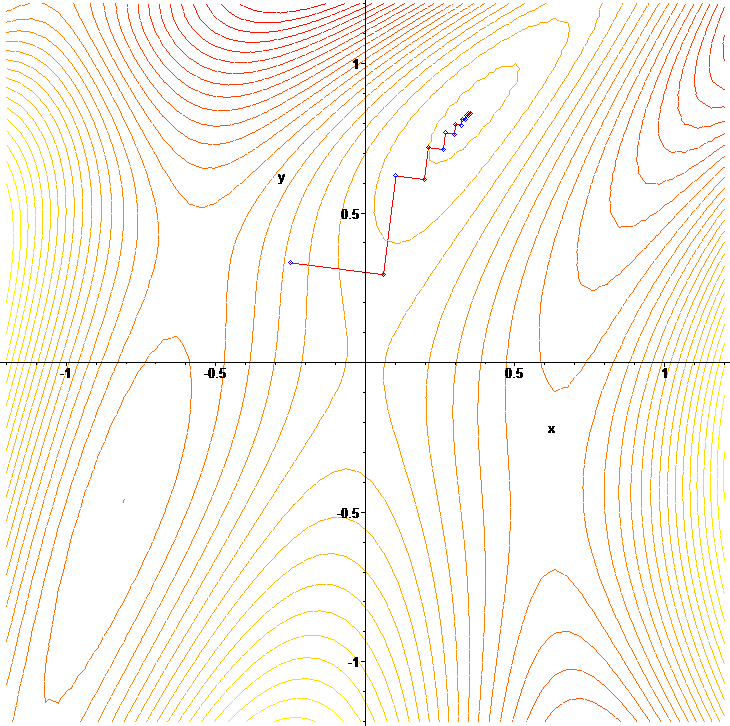
\includegraphics[width=0.45\textwidth]{images/gradient_ascent_contour.png}
  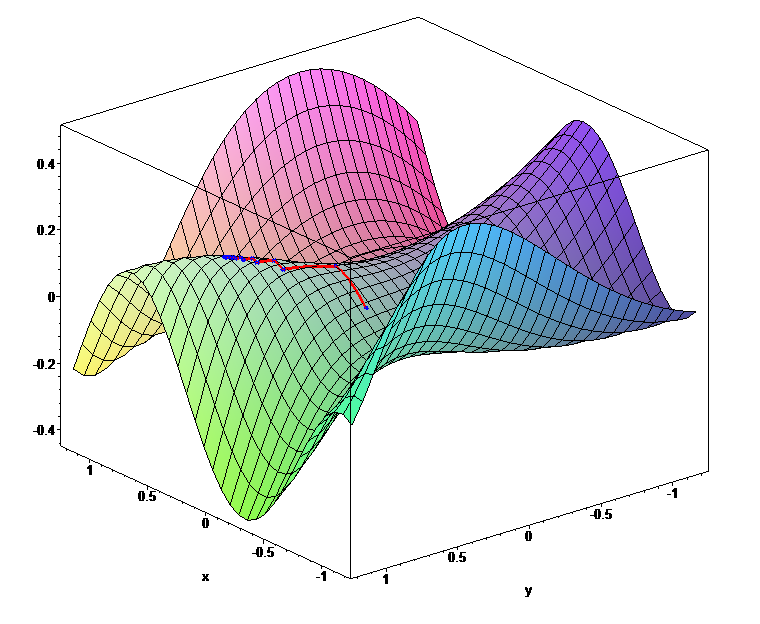
\includegraphics[width=0.45\textwidth]{images/gradient_ascent_surface.png}
  \caption{\label{fig:grad-desc}Visualización de la técnica de gradiente descendente, en este caso, buscando un máximo de la función $F(x,y)=\sin\left(\frac{1}{2} x^2 - \frac{1}{4} y^2 + 3 \right) \cos(2 x+1-e^y)$. Imágenes de Wikimedia Commons en dominio público}
\end{figure}

La técnica de gradiente descendente presenta algunos problemas: como se
puede observar en la figura \ref{fig:grad-desc}, cuando el gradiente de
la función es próximo a cero el algoritmo tiende a dar pasos muy cortos,
convergiendo muy lentamente hacia el extremo local encontrado. Asimismo,
en general puede presentar un comportamiento de ``zig-zag'' para ciertas
funciones, avanzando de forma casi ortogonal al segmento que guarda la
distancia más corta con el extremo.


\chapter{Deep Learning}\label{ch:deep}

En este capítulo nos centramos en el ámbito de las técnicas que aplicaremos
en la práctica, el Deep Learning. Estas técnicas están basadas en redes neuronales, de las que introducimos algunos aspectos al hablar de las redes prealimentadas profundas. Se describen y se clasifican las unidades que las componen. Posteriormente, se expone el proceso de evaluación de una red de este tipo mediante la propagación hacia adelante y hacia atrás. Además, se especifican los algoritmos derivados de gradiente descendente que permiten realizar aprendizaje sobre ellas. Por último, se definen las estructuras principales de redes que efectúan un aprendizaje no supervisado sobre los datos.

\section{Redes neuronales prealimentadas
profundas}\label{redes-neuronales-prealimentadas-profundas}

\label{sec:feedforward}

Las redes prealimentadas profundas, también conocidas como perceptrones
multicapa o en inglés como \emph{deep feedforward neural networks}, son
el modelo canónico de aprendizaje profundo \autocite{goodfellow2016}. El
objetivo de una red prealimentada es aproximar una función \(f^{*}\),
definiendo una aplicación \(f(x;\theta)\) y aprendiendo el valor de los
parámetros \(\theta\) que resultan en la mejor aproximación.

En concreto, las redes prealimentadas se caracterizan por que no se
forman ciclos en las conexiones entre unidades. Así, la información se
evalúa siempre hacia adelante a través de las conexiones intermedias
usadas para definir \(f\), hasta la salida de la red. No hay
retroalimentaciones en las que salidas de algunas unidades de la red
vuelvan a ser entradas del modelo.

Estas redes se suelen representar como una composición en cadena de
varias funciones, que se puede asociar a un grafo acíclico. Por ejemplo,
podríamos tener una red composición de funciones vectoriales
\(f_1, f_2, f_3\) de la siguiente forma: \(f(x)=f_3(f_2(f_1(x)))\). En
este caso, decimos que \(f_1\) es la primera capa, \(f_2\) la segunda
capa y \(f_3\) la capa de salida. Las capas que no corresponden a la
salida de \(f\) se suelen denominar \emph{capas ocultas}. La longitud de
esta cadena nos da la profundidad del modelo.

A diferencia de otros algoritmos de aprendizaje automático, las redes
neuronales mantienen esta estructura de capas de forma que la capa
\(i+1\)-ésima únicamente opera con los datos de salida de la
\(i\)-ésima; en particular, sólo la primera capa utiliza directamente
los datos de entrada. Además, por la inspiración biológica de las redes,
cada componente de cada capa (\emph{unidad}) se puede interpretar como
una neurona. Las neuronas de los seres vivos se componen de dendritas que recogen estímulos de otras neuronas, un núcleo que los acumula y un axón con terminales que se conectan a otras neuronas y le permiten transmitir nuevos impulsos. Se ejemplifica esta estructura en la \autoref{fig:neuron}.

\begin{figure}[hbtp]
  \centering
  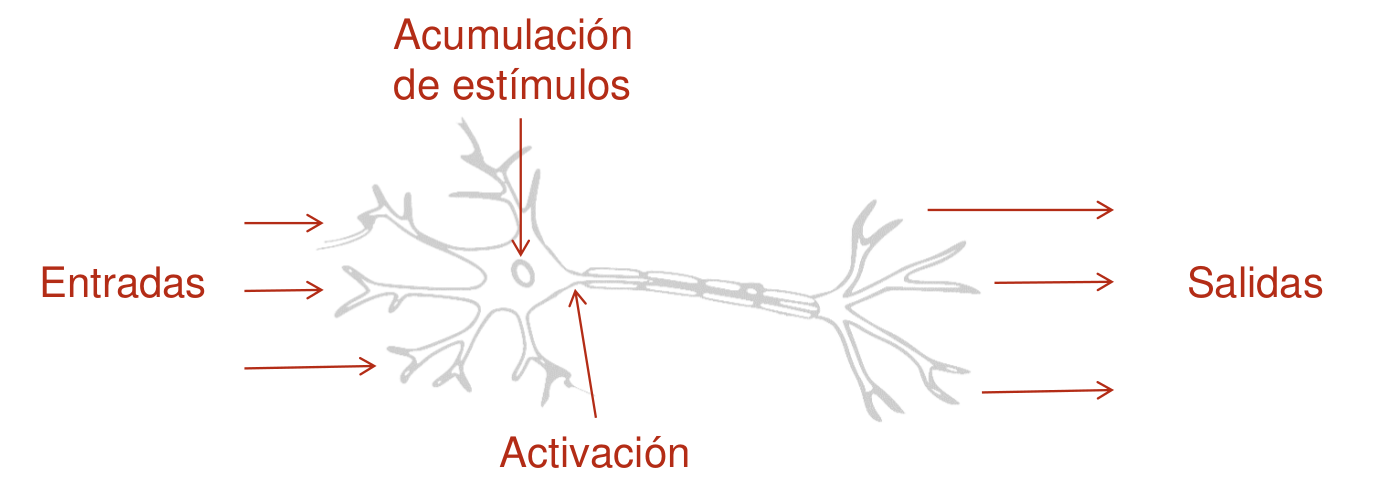
\includegraphics[width=\textwidth]{images/neurona_biologica}
  \caption[Neurona biológica]{Ilustración de una neurona biológica, indicando las equivalencias con la neurona artificial}
  \label{fig:neuron}
\end{figure}

\begin{figure}[hbtp]
  \centering
  
\begin{tikzpicture}[scale=0.2]
\tikzstyle{every node}+=[inner sep=0pt]
\draw [black] (39.4,-29) circle (5.5);
\draw (39.4,-29) node {$g(\Tr wx+b)$};
%\draw (51.6,-29) node {$f$};
\draw [black] (44.9,-29) -- (48.6,-29);
\fill [black] (48.6,-29) -- (47.8,-28.5) -- (47.8,-29.5);

\draw (15.9,-20.2) node {$x_1$};
\draw (15.9,-36.7) node {$x_m$};
\draw (15.9,-30.9) node {$\vdots$};
\draw (15.9,-26) node {$x_2$};
\draw [black] (18.66,-21.37) -- (33.84,-27.83);
\fill [black] (33.84,-27.83) -- (33.3,-27.05) -- (32.91,-27.97);
\draw (24.55,-25.12) node [below] {$w_1$};
\draw [black] (18.87,-26.43) -- (33.63,-28.57);
\fill [black] (33.63,-28.57) -- (32.91,-27.96) -- (32.77,-28.95);
\draw (25.63,-28.16) node [below] {$w_2$};
\draw [black] (18.71,-35.65) -- (33.79,-30.05);
\fill [black] (33.79,-30.05) -- (32.86,-29.86) -- (33.21,-30.79);
\draw (28.87,-33.42) node [below] {$w_m$};
\end{tikzpicture}

  \caption[Neurona artificial]{Una neurona artificial con $m$ entradas y función de activación $g$}
  \label{fig:art-neuron}
\end{figure}

La analogía se lleva a la neurona artificial, como se muestra en la \autoref{fig:art-neuron}, mediante una función de \(\RR^{m}\) en \(\RR\),
donde \(m\) es el número de unidades en la capa anterior. El
comportamiento es similar a una neurona en el sentido de que recoge
información de varias unidades cercanas y calcula su propio valor de
activación, así como la estructuración en capas se ha tomado de la
neurociencia. En la figura \ref{fig:dfnn} se muestra una representación
común de una red neuronal como unidades conectadas formando un grafo.
Las flechas indican el sentido en el que viajan los datos, es decir, las
salidas de funciones que se toman como entradas de otras funciones.

\begin{figure}[hbtp]
  \centering
\begin{tikzpicture}[scale=0.2]
\tikzstyle{every node}+=[inner sep=0pt]
\draw [black] (21.5,-13.4) circle (3);
\draw [black] (21.5,-23.4) circle (3);
\draw [black] (21.5,-33.1) circle (3);
\draw [black] (36.4,-7.6) circle (3);
\draw [black] (36.4,-17.8) circle (3);
\draw [black] (36.4,-28.2) circle (3);
\draw [black] (36.4,-39.6) circle (3);
\draw [black] (50.6,-23.4) circle (3);
\draw [black] (24.35,-32.16) -- (33.55,-29.14);
\fill [black] (33.55,-29.14) -- (32.63,-28.91) -- (32.95,-29.86);
\draw [black] (24.25,-34.3) -- (33.65,-38.4);
\fill [black] (33.65,-38.4) -- (33.12,-37.62) -- (32.72,-38.54);
\draw [black] (23.59,-30.95) -- (34.31,-19.95);
\fill [black] (34.31,-19.95) -- (33.39,-20.17) -- (34.11,-20.87);
\draw [black] (23.01,-30.51) -- (34.89,-10.19);
\fill [black] (34.89,-10.19) -- (34.05,-10.63) -- (34.91,-11.13);
\draw [black] (23.56,-21.22) -- (34.34,-9.78);
\fill [black] (34.34,-9.78) -- (33.43,-10.02) -- (34.16,-10.71);
\draw [black] (24.31,-22.34) -- (33.59,-18.86);
\fill [black] (33.59,-18.86) -- (32.67,-18.67) -- (33.02,-19.6);
\draw [black] (24.36,-24.32) -- (33.54,-27.28);
\fill [black] (33.54,-27.28) -- (32.94,-26.56) -- (32.63,-27.51);
\draw [black] (23.53,-25.61) -- (34.37,-37.39);
\fill [black] (34.37,-37.39) -- (34.2,-36.46) -- (33.46,-37.14);
\draw [black] (24.3,-12.31) -- (33.6,-8.69);
\fill [black] (33.6,-8.69) -- (32.68,-8.51) -- (33.04,-9.44);
\draw [black] (24.38,-14.25) -- (33.52,-16.95);
\fill [black] (33.52,-16.95) -- (32.9,-16.24) -- (32.61,-17.2);
\draw [black] (23.63,-15.51) -- (34.27,-26.09);
\fill [black] (34.27,-26.09) -- (34.06,-25.17) -- (33.35,-25.88);
\draw [black] (22.98,-16.01) -- (34.92,-36.99);
\fill [black] (34.92,-36.99) -- (34.96,-36.05) -- (34.09,-36.54);
\draw [black] (38.41,-9.83) -- (48.59,-21.17);
\fill [black] (48.59,-21.17) -- (48.43,-20.24) -- (47.69,-20.91);
\draw [black] (39.19,-18.9) -- (47.81,-22.3);
\fill [black] (47.81,-22.3) -- (47.25,-21.54) -- (46.88,-22.47);
\draw [black] (39.24,-27.24) -- (47.76,-24.36);
\fill [black] (47.76,-24.36) -- (46.84,-24.14) -- (47.16,-25.09);
\draw [black] (38.38,-37.34) -- (48.62,-25.66);
\fill [black] (48.62,-25.66) -- (47.72,-25.93) -- (48.47,-26.59);
\end{tikzpicture}
\caption{\label{fig:dfnn}Ilustración ejemplificando una red neuronal prealimentada de tres capas}
\end{figure}

Para entender cómo las redes prealimentadas aproximan funciones,
consideremos algunos modelos lineales como la regresión lineal o la
logística. Estos modelos tienen claras ventajas, son sencillos, se
pueden ajustar de forma eficiente y fiable. Sin embargo, están muy
limitados, dado que sólo tiene sentido aplicarlos a funciones lineales,
por lo que no pueden sintetizar interacciones entre dos variables de
entrada.

Cuando el objetivo es aproximar funciones no lineales, una vía es
aplicar un modelo lineal no a la variable independiente sino a una
transformación no lineal de la misma. El problema se traduce entonces en
qué transformación \(\phi\) de la variable aplicar para que el modelo
lineal tenga un buen ajuste. Frente a buscar \(\phi\) manualmente, que
requiere extenso conocimiento de cada problema, o usar un \(\phi\) de
muy alta dimensionalidad con capacidad para todos los ejemplos del
conjunto de datos, las redes neuronales realizan un aprendizaje de
\(\phi\) entre una clase de funciones parametrizada: se define un modelo
del tipo

\begin{equation}
  f^{*}(x)\approx f(x;\theta,w)=\Tr{\phi(x;\theta)}w, 
\end{equation}
donde \(\theta\) es un vector de parámetros que facilita escoger una
función \(f\) concreta de entre la clase que define, y \(w\) es otro
vector de parámetros que permite aplicar la transformación obtenida en
la salida deseada. Para encontrar los parámetros que corresponden a una
buena aproximación, se utilizará un algoritmo de optimización basado en
la técnica de gradiente descendente presentada en la sección
\ref{sec:grad-desc}. Se trata de un enfoque muy flexible, ya que se
puede proveer al algoritmo de una clase de funciones más general o más
concreta, según el conocimiento sobre el problema que se posea.

La clase de funciones, dentro de la cual una red neuronal busca la
aproximación, se determina escogiendo la estructura de la red y los
tipos de unidades ocultas y de salida.

\subsection{Funciones de coste}\label{sec:funciones-de-coste}

La mayoría de diseños de redes neuronales involucran definir una
distribución \(P(y\mid x;\theta)\) y aplicar el principio de máxima
verosimilitud. En otros casos, mediante funciones de coste específicas,
se puede predecir simplemente algún estadístico de \(y\) condicionado a
\(x\), en lugar de determinar una distribución de probabilidad.

En el caso más habitual, la función de coste se definirá como la
entropía cruzada (equivalentemente, la log-verosimilitud negativa) entre
la distribución de los datos, \(\hat p\), y la del modelo, \(p\), y
sobre la variable de la salida generada \(y\) respecto de la entrada
\(x\):
\[J(\theta)=C(\hat p(y\mid x), p(y\mid x))=-\E_{\hat p}[\log p(y\mid x)].\]
Una ventaja de este enfoque es que esta función de coste viene determinada
automáticamente por el modelo \(p(y\mid x)\) que escojamos y evita tener
que definir una nueva función para cada modelo. Además, la entropía
cruzada suele permitir calcular gradientes relativamente ``grandes'', en
el sentido de que no se acercan rápidamente a cero, lo cual beneficia al
proceso de optimización.

En ocasiones se añade a la función de coste un término de regularización
o \emph{decaimiento de pesos} de forma que el coste total queda:
\[J(\theta)=C(\hat p, p;y\mid x) + \lambda \Omega(\theta)\]

\subsection{Unidades de salida}\label{unidades-de-salida}

La expresión concreta de la función de coste, cuando la tomamos como la
entropía cruzada, vendrá determinada por la representación de la salida
de la red prealimentada. Estudiamos a continuación el tipo de unidades
que se suelen utilizar para dar dicha salida. Durante el resto de esta
sección, supondremos que la red proporciona un vector de características
\(h=f(x;\theta)\) generado por las unidades ocultas. El cometido de las
unidades de salida es dar una transformación que aporte una salida
apropiada.

\subsubsection{Unidades lineales}\label{unidades-lineales}

Una capa de unidades de este tipo realiza una transformación afín de los
datos: \(\hat y=\Tr Wh+b\). Se suelen utilizar para calcular la media de
una distribución condicional normal: \[p(y\mid x)=\PN(y;\hat t,I).\] En
ese caso, maximizar la entropía cruzada es equivalente a minimizar el
error cuadrático medio.

\subsubsection{Unidades con activación
sigmoidal}\label{unidades-con-activaciuxf3n-sigmoidal}
En muchas tareas, la variable objetivo \(y\) es de tipo binario. Por
ejemplo, los problemas de clasificación binaria son un caso particular
de esta situación. La técnica de máxima verosimilitud lleva a definir
una distribución de Bernoulli sobre \(y\) condicionada a \(x\). Esta
distribución está determinada por un único número en el intervalo
\([0, 1]\), que se corresponde con \(P(y=1\mid x)\).

Para que la unidad de salida tenga un buen comportamiento, es necesario
que no genere gradiente $0$ ni muy cercano a $0$ en casos en los que el
modelo no se acerque a una solución. Esto se consigue utilizando una
\emph{función de activación}, es decir, se compone el cómputo de la
unidad con otra función que la regulariza de alguna manera. En este
caso, se utiliza la función logística:
\[z=\Tr wh+b;\ \hat y = \sigma(z) = \frac{1}{1+e^{-z}}\]

En la \autoref{fig:sigm} se observan los valores en los que se aplica $\sigma$ según el valor de $z$.

\begin{figure}[hbtp]
  \centering
  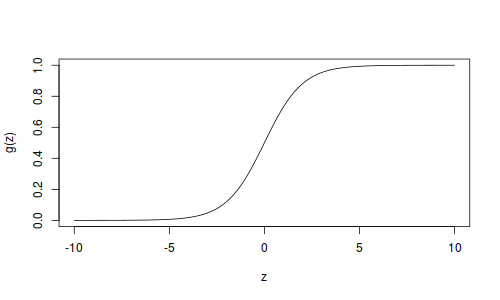
\includegraphics[width=0.7\textwidth]{images/sigmoid.png}
  \caption[Logística]{Gráfica de la función logística}
  \label{fig:sigm}
\end{figure}

Definamos ahora una distribución de probabilidad sobre \(y\), usando el
valor \(z\). Podemos comenzar asumiendo que la probabilidad no
normalizada \(\tilde P\) es log-lineal en \(z\) e \(y\):
\[\log \tilde P(y)=yz,\] y exponenciamos \[\tilde P(y)=e^{yz},\] para
ahora normalizar sobre los valores de \(\tilde P\), obteniendo una
probabilidad \[P(y)=\frac{e^{yz}}{e^{0z}+e^{1z}}=\frac{e^{yz}}{1+e^z}\]
y utilizando de nuevo que \(y\in\{0,1\}\) se tiene

\begin{equation}\label{eq:sigm-prob}
  P(y)=\frac{e^{yz}}{e^{(1-y)z}+e^{yz}}=\frac{1}{\frac{e^{z}}{e^{2yz}}+1}=\sigma((2y-1)z).
\end{equation}

El resultado es una distribución de Bernoulli determinada por una
transformación logística de \(z\). De hecho, puesto que los posibles
valores de \(y\) son $0$ y $1$, también podemos expresarla más claramente
como:
\[P(y)=\sigma(z)^y\sigma(-z)^{1-y}=p^y(1-p)^{1-y}\mbox{ donde }p=\sigma(z).\]

Ahora, la función de coste para esta distribución, tomando la entropía
cruzada y usando \eqref{eq:sigm-prob}, es:
\[J(\theta)=-\log P(y\mid x)=-\log\sigma((2y-1)z).\]

Dado que la función logística está valuada en el intervalo abierto
\(]0,1[\), su logaritmo es finito y \(J\) está bien definida.

\subsubsection{\texorpdfstring{Unidades con activación
\emph{softmax}}{Unidades con activación softmax}}\label{unidades-con-activaciuxf3n-softmax}

Las unidades con función de activación \emph{softmax} se emplean cuando
se pretende representar una distribución de probabilidad sobre una
variable discreta con un número finito de valores. Generalmente, esta
situación se da en problemas de clasificación multiclase. Así, se pueden
interpretar como una generalización de las unidades sigmoidales.

Mientras que para caracterizar una variable binaria bastaba con una sola
unidad de salida (la salida era un escalar entre $0$ y $1$), ahora se
utilizarán tantas unidades como posibles valores puedar tomar la variable. Si
\(y\) puede tomar uno de entre \(n\) posibles valores, la capa de salida
con \emph{softmax} generará un vector \(\hat y\) donde
\(\hat y_i=P(y=i\mid x)\), exigiendo que \(\sum_{i=1}^n\hat y_i=1\).

La función vectorial \emph{softmax} se define en cada componente
\(i=1,\dots,n\) como

\begin{equation}\label{eq:softmax}
  \softmax{z}_i = \frac{\exp(z_i)}{\sum_{j=1}^{n}\exp(z_j)}.
\end{equation}

El vector \(z\) al que se aplica la función se obtiene de una capa de
unidades lineales que proporcionan probabilidades logarítmicas sin
normalizar:
\[z=\Tr Wh+b;\ z_{i}=\log\tilde P(y=i\mid x).\]

De nuevo, la
función de coste se puede definir siguiendo la misma técnica, mediante
la entropía cruzada.

\subsection{Unidades ocultas}\label{unidades-ocultas}

Cualquiera de los tipos anteriores de unidad se puede utilizar en una
capa oculta, pero existen más y el diseño de unidades ocultas es un
campo de investigación muy activo, pese a la falta de principios
teóricos que lo guíen. A continuación se exponen algunos de los tipos
más usuales. Salvo que se indique lo contrario, todas las capas de
unidades calculan una transformación afín \[z= \Tr Wx+b,\] donde \(x\) es
el vector de entrada, equivalentemente, el vector de salida de la capa
inmediatamente anterior o un vector de datos si se trata de la primera
capa. Se compone esta transformación con la función de activación
específica a cada tipo de unidad.

\subsubsection{Unidades lineales rectificadas
(ReLU)}\label{unidades-lineales-rectificadas-relu}

La función de activación de las unidades lineales rectificadas
(\emph{Rectified Linear Units}, ReLU) es

\begin{equation}
g(z)_i=\max\{0,z_i\}.
\end{equation}

Se muestra en la \autoref{fig:relu} el valor que toma la ReLU según el valor de $z_i$.

\begin{figure}[hbtp]
  \centering
  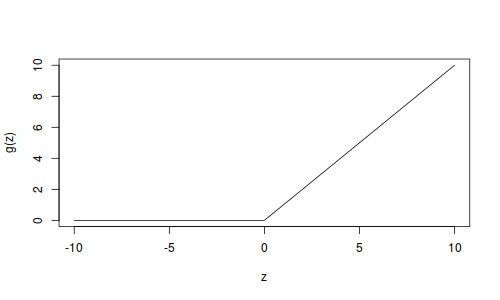
\includegraphics[width=0.7\textwidth]{images/relu.png}
  \caption[ReLU]{Gráfica de la función de activación de una ReLU}
  \label{fig:relu}
\end{figure}

Estas unidades son fáciles de optimizar ya que son similares a las
unidades lineales. Aunque no es diferenciable en \(z=0\), se pueden
utilizar algoritmos basados en gradiente para optimizar la función
objetivo. Esto es debido a que, generalmente, durante el entrenamiento
no se llega a un punto en el que el gradiente sea exactamente $0$, así que
se pueden aceptar puntos donde el gradiente no esté definido en los
mínimos de la función coste.

\subsubsection{Extensiones de ReLU}\label{extensiones-de-relu}

Algunas generalizaciones de las ReLU modifican el gradiente cuando las
componentes de \(z\) son negativas:

\begin{itemize}
\tightlist
\item
  \textbf{Rectificación por valor absoluto}:
  \(g(z)_{i}=\lvert z_{i} \rvert\)
\item
  \textbf{\emph{Leaky} ReLU}: \(g(z)_i=\max(0,z_i)+\alpha\min(0,z_i)\)
  con \(\alpha\) pequeño como \(0,01\) (\autoref{fig:leaky})
\item
  \textbf{ReLU paramétrica}: \(g(z)_i=\max(0,z_i)+\alpha_i\min(0,z_i)\),
  con \(\alpha_i\) como un parámetro optimizable
\end{itemize}

\begin{figure}[hbtp]
  \centering
  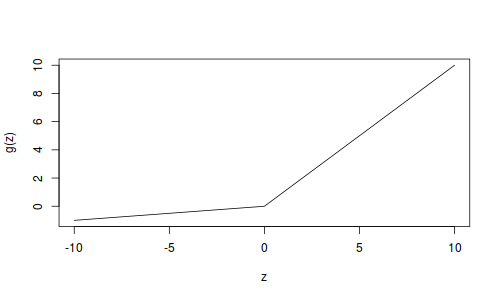
\includegraphics[width=0.7\textwidth]{images/leaky.png}
  \caption[Leaky ReLU]{Función de activación de una \emph{leaky} ReLU para $\alpha=0.1$}
  \label{fig:leaky}
\end{figure}

Las capas de \textbf{unidades \emph{maxout}} agrupan las componentes de
\(z\) en conjuntos de \(k\) valores cada uno. Cada una de las unidades
de la capa proporciona entonces el máximo de uno de esos conjuntos:
\[g(z)_i=\max\{z_j:j\in S_i\},\ S_i=\{(i-1)k + 1, (i-1)k + 2,\dots, ik\}.\]
En este caso, si \(z\in\RR^{kd}\), entonces \(g(z)\in\RR^{d}\). El
aspecto interesante de las unidades \emph{maxout} es el hecho de que una
capa de ellas puede aprender una función convexa lineal a trozos de
hasta \(k\) trozos. Podemos intuir que una capa de este tipo podrá
aproximar cualquier función convexa con precisión arbitraria para un
\(k\) conveniente.

\subsubsection{Unidades con activación sigmoidal o tangente
hiperbólica}\label{unidades-con-activaciuxf3n-sigmoidal-o-tangente-hiperbuxf3lica}

Otras dos funciones muy comunes para la activación de unidades en redes
neuronales son la función logística

\begin{equation}
  g(z)_i=\sigma(z_i)=\frac{1}{1+e^{-z_i}},
\end{equation}
y la tangente hiperbólica (\autoref{fig:tanh})
\begin{equation}
  g(z)_i=\tanh(z_i)=\frac{e^{z_i}-e^{-z_i}}{e^{z_i}+e^{-z_i}}.
\end{equation}

\begin{figure}[hbtp]
  \centering
  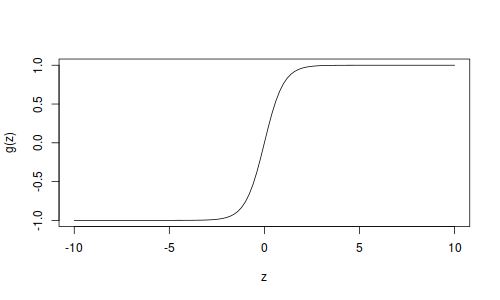
\includegraphics[width=0.7\textwidth]{images/tanh.png}
  \caption[$\tanh$]{Gráfica de la función tangente hiperbólica}
  \label{fig:tanh}
\end{figure}

Se puede comprobar que \(\tanh(z_i)=2\sigma(2z_i)-1\).

El uso de estas unidades era más común antes de la aparición de las
ReLU. En la actualidad está decreciendo su uso.

\subsubsection{Otras unidades ocultas}\label{otras-unidades-ocultas}

Para construir otros tipos de unidad oculta simplemente basta con elegir
otra función de activación. Las siguientes son algunas relativamente
comunes:

\begin{itemize}
\tightlist
\item
  El \textbf{coseno} \(g(z)_i=cos(z_i)\) ha sido usada por
  \textcite{goodfellow2016} en el conocido conjunto MNIST obteniendo una
  tasa de error inferior al 1\%.
\item
  La \textbf{identidad} \(g(z) = z\) se puede utilizar para encadenar
  capas de forma lineal y utilizar alguna función de activación
  diferente a la salida.
\item
  La función \emph{softplus} \(g(z)_i=\zeta(z_i)=\log(1+e^{z_i})\) es
  una versión infinitamente derivable de la unidad lineal rectificada (\autoref{fig:softplus}).
  Sin embargo, en la práctica no suele presentar ventajas sobre la ReLU.
\end{itemize}

\begin{figure}[hbtp]
  \centering
  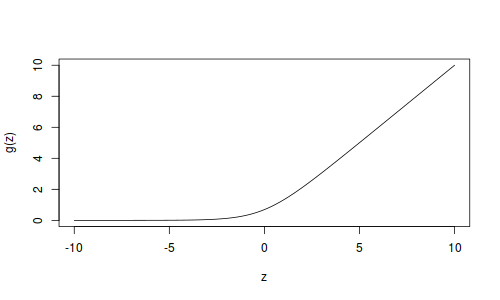
\includegraphics[width=0.7\textwidth]{images/softplus.png}
  \caption[Softplus]{Gráfica de la función \emph{softplus}}
  \label{fig:softplus}
\end{figure}

\section{Entrenamiento de redes neuronales
profundas}\label{entrenamiento-de-redes-neuronales-profundas}

El proceso de entrenamiento de una red neuronal profunda
requiere realizar observaciones sobre las salidas a partir de los datos
de entrada, y evaluar el error cometido respecto a las salidas deseadas.
Para calcular la salida de la red $f(x)$ frente a una instancia $x$ se
utiliza el mecanismo de propagación hacia adelante, en el que intuitivamente
podemos decir que los datos ``atraviesan'' la red. La evaluación de la
red se realiza en base a una función de coste y posteriormente se deben
actualizar los parámetros para alterar la función $f$, para lo cual es
necesario calcular el gradiente de dicho coste. El cómputo del gradiente
se obtiene mediante la técnica de propagación hacia atrás.

\subsection{Propagación hacia
adelante}\label{propagaciuxf3n-hacia-adelante}

Las redes neuronales prealimentadas, que se han estudiado en la sección
\ref{sec:feedforward}, son funciones que aceptan vectores de entrada y
procesan la información computando varias funciones intermedias,
propagando así la información, hasta la salida de la red. Este proceso
se denomina \emph{propagación hacia adelante}, y se describe en el
algoritmo \ref{alg:fwdprop}.

\begin{algorithm}
\caption{Propagación hacia adelante en una red neuronal profunda con función de activación $g$, y cálculo de la función de coste $J$, para una instancia $x$ (en la práctica se utilizan minilotes de instancias)}
\label{alg:fwdprop}
\begin{algorithmic}
  \REQUIRE{profundidad de la red $l$}
  \REQUIRE{$W^{(i)}$ matriz de pesos de la capa $i$-ésima}
  \REQUIRE{$b^{(i)}$ vector de sesgos de la capa $i$-ésima}
  \REQUIRE{instancia $x$ a procesar}
  \REQUIRE{salida objetivo $y^{*}$}
  \STATE{$h^{(0)}\gets x$}
  \FOR{$k=1,\dots,l$}
  \STATE{$z^{(k)}\gets W^{(k)}h^{(k-1)}+b^{(k)}$}
  \STATE{$h^{(k)}\gets g(z^{(k)})$}
  \ENDFOR
  \STATE{$y\gets h^{(l)}$}
  \STATE{Se calcula la función de coste mediante una distancia o pérdida entre la salida obtenida y la deseada, y un término de regularización $\Omega$:}
  \STATE{$J\gets L(y,y^{*})+\lambda \Omega(\theta)$}
\end{algorithmic}
\end{algorithm}

\subsection{Propagación hacia
atrás}\label{sec:backprop}

Consideremos una red neuronal prealimentada profunda, determinada por un
vector de parámetros \(\theta\). Durante el entrenamiento, la salida
generada por la propagación hacia adelante se compara con la salida
deseada y se calcula un coste \(J(y,y^{*};\theta)\in\RR\). Para aplicar
un algoritmo de optimización basado en gradiente descendente (se
estudiarán en la sección \ref{sec:dl-opt}), es necesario conocer el
gradiente de la función \(J\) respecto de los parámetros \(\theta\).
Este gradiente se puede calcular analíticamente, pero evaluar
\(\nabla_{\theta} J(y,y^{*};\theta)\) es generalmente muy costoso
computacionalmente. El algoritmo de propagación hacia atrás, o
\emph{backprop}, realiza este cálculo de forma eficiente.

\begin{example}
  
Consideremos la red neuronal de la figura \ref{fig:ex-backprop}. Suponiendo que cada neurona utiliza la misma función de activación $g$, podemos dar una expresión de $f$ acorde con los pesos y sesgos que se muestran en la imagen.

  \begin{figure}[hbtp]
\centering
\begin{tikzpicture}[scale=0.2]
\tikzstyle{every node}+=[inner sep=0pt]
\draw [black] (34,-24.7) circle (3);
\draw [black] (34,-38.8) circle (3);
\draw [black] (48.7,-33) circle (3);
\draw (15.2,-24.7) node {$x_1$};
\draw (15.2,-38.8) node {$x_2$};
\draw (61.1,-33) node {$f$};
\draw (23.8,-13.6) node {$1$};
\draw (41.5,-13.6) node {$1$};
\draw [black] (36.79,-37.7) -- (45.91,-34.1);
\fill [black] (45.91,-34.1) -- (44.98,-33.93) -- (45.35,-34.86);
\draw (43.4,-36.44) node [below] {$w_{12}^{(2)}$};
\draw [black] (36.61,-26.18) -- (46.09,-31.52);
\fill [black] (46.09,-31.52) -- (45.64,-30.7) -- (45.15,-31.57);
\draw (39.21,-29.35) node [below] {$w_{11}^{(2)}$};
\draw [black] (17.6,-26.5) -- (31.6,-37);
\fill [black] (31.6,-37) -- (31.26,-36.12) -- (30.66,-36.92);
\draw (19.45,-29.25) node [below] {$w_{21}^{(1)}$};
\draw [black] (17.6,-37) -- (31.6,-26.5);
\fill [black] (31.6,-26.5) -- (30.66,-26.58) -- (31.26,-27.38);
\draw (22.75,-33.50) node [below] {$w_{12}^{(1)}$};
\draw [black] (51.7,-33) -- (58.1,-33);
\fill [black] (58.1,-33) -- (57.3,-32.5) -- (57.3,-33.5);
\draw [black] (25.83,-15.81) -- (31.97,-22.49);
\fill [black] (31.97,-22.49) -- (31.8,-21.56) -- (31.06,-22.24);
\draw (31.36,-16.61) node [left] {$b_1^{(1)}$};
\draw [black] (42.54,-16.41) -- (47.66,-30.19);
\fill [black] (47.66,-30.19) -- (47.85,-29.26) -- (46.91,-29.61);
\draw (44.34,-24.11) node [left] {$b_1^{(2)}$};
\draw [black] (24.93,-16.38) -- (32.87,-36.02);
\fill [black] (32.87,-36.02) -- (33.04,-35.09) -- (32.11,-35.47);
\draw (25.16,-20.1) node [left] {$b_2^{(1)}$};
\draw [black] (18.2,-24.7) -- (31,-24.7);
\fill [black] (31,-24.7) -- (30.2,-24.2) -- (30.2,-25.2);
\draw (24.6,-25.2) node [below] {$w_{11}^{(1)}$};
\draw [black] (18.2,-38.8) -- (31,-38.8);
\fill [black] (31,-38.8) -- (30.2,-38.3) -- (30.2,-39.3);
\draw (24.6,-39.3) node [below] {$w_{22}^{(1)}$};
\end{tikzpicture}
\caption{\label{fig:ex-backprop}Red neuronal sencilla de dos capas con entrada vectorial de dos componentes, se marcan los pesos y los sesgos en cada conexión}
\end{figure}

En este caso, el vector de parámetros que determina la red será
$$\theta=\left(w_{11}^{(1)},w_{12}^{(1)},w_{21}^{(1)},w_{22}^{(1)},b_{1}^{(1)},b_{2}^{(1)},w_{11}^{(2)},w_{12}^{(2)},b_{1}^{(2)}\right).$$
Puesto que la función de coste $J$ vendrá determinada por el valor de $f$ en el mismo punto, para calcular su gradiente nos interesa conocer el de $f$. La expresión desarrollada de $f$ queda\footnotesize
\begin{gather*}
f(x_1,x_2;\theta)=\\g\left(w_{11}^{(2)}g\left(w_{11}^{(1)}x_{1}+w_{12}^{(1)}x_2+b_1^{(1)}\right)+w_{12}^{(2)}g\left(w_{21}^{(1)}x_1+w_{22}^{(1)}x_2+b_2^{(1)}\right)+b_1^{(2)}\right).
\end{gather*}\normalsize

Ahora, mediante la regla de la cadena podemos desarrollar la parcial de $f$ respecto de cualquiera de los parámetros. Llamamos
\footnotesize
\begin{align*}
  \alpha&=g'\left(w_{11}^{(2)} g\left(w_{11}^{(1)}x_{1}+w_{12}^{(1)}x_2+b_1^{(1)}\right) + w_{12}^{(2)} g\left(w_{21}^{(1)}x_1+w_{22}^{(1)}x_2+b_2^{(1)}\right)+b_1^{(2)}\right)\\
  \beta&=g'\left(w_{11}^{(1)}x_{1}+w_{12}^{(1)}x_2+b_1^{(1)}\right)\\
  \gamma&=g'\left(w_{21}^{(1)}x_{1}+w_{22}^{(1)}x_2+b_2^{(1)}\right)
\end{align*}
\normalsize
y se tiene
\footnotesize
\begin{alignat*}{3}
  \frac{\partial f}{\partial w_{11}^{(1)}}(x_1,x_2;\theta)&=\alpha w_{11}^{(2)}\beta x_1,\quad&
  \frac{\partial f}{\partial w_{12}^{(1)}}(x_1,x_2;\theta)&=\alpha w_{11}^{(2)}\beta x_2,\\
  \frac{\partial f}{\partial w_{21}^{(1)}}(x_1,x_2;\theta)&=\alpha w_{12}^{(2)}\gamma x_1,\quad&
  \frac{\partial f}{\partial w_{22}^{(1)}}(x_1,x_2;\theta)&=\alpha w_{12}^{(2)}\gamma x_2,\\
  \frac{\partial f}{\partial b_{1}^{(1)}}(x_1,x_2;\theta)&=\alpha w_{11}^{(2)}\beta, \quad&
  \frac{\partial f}{\partial b_{2}^{(1)}}(x_1,x_2;\theta)&=\alpha w_{12}^{(2)}\gamma, \\
  \frac{\partial f}{\partial w_{11}^{(2)}}(x_1,x_2;\theta)&=\alpha g(w_{11}^{(1)}x_{1}+w_{12}^{(1)}x_2 + b_1^{(1)}),&&\\
  \frac{\partial f}{\partial w_{12}^{(2)}}(x_1,x_2;\theta)&=\alpha g(w_{21}^{(1)}x_{1}+w_{22}^{(1)}x_2 + b_2^{(1)}),&\quad
  \frac{\partial f}{\partial b_{1}^{(2)}}(x_1,x_2;\theta)&=\alpha.
\end{alignat*}
\normalsize

Como podemos observar, algunos de los factores de las parciales se repiten en varias de ellas, de forma que se ahorrarán muchos cálculos innecesarios si no se repiten. Este hecho se hace aún más evidente conforme se añaden capas a la red y unidades a cada capa. Por ello, el algoritmo de propagación hacia atrás permite optimizar el cálculo del gradiente mediante varios pasos intermedios para evitar cálculos repetidos.

\end{example}

En el algoritmo \ref{alg:backprop} se describe \emph{backprop} paso a
paso. Es fácil comprobar que aplicando esta técnica al ejemplo anterior
podemos evaluar las parciales que se han deducido sin repetir cálculos
costosos.

\begin{algorithm}
\caption{Propagación hacia atrás}
\label{alg:backprop}
\begin{algorithmic}
\STATE{Tras la propagación hacia adelante, calcular el gradiente de la capa de salida:}
\STATE{$d\gets \nabla_{y}J(y,y^{*};\theta)=\nabla_{y}L(y,y^{*})$}
  \FOR{$k=l,\dots,1$}
  \STATE{Aplicar la regla de la cadena a la función de activación ($\odot$ denota producto componente a componente):}
  \STATE{$d\gets \nabla_{z^{(k)}}J=d\odot g'(z^{i})$}
  \STATE{Calcular gradientes en los pesos y sesgos (incluyendo el término de regularización si es necesario):}
  \STATE{$\nabla_{b^{(k)}}J=d+\lambda\nabla_{b^{(k)}}\Omega(\theta)$}
  \STATE{$\nabla_{W^{(k)}}J=d\Tr{(h^{(k-1)})}+\lambda\nabla_{W^{(k)}}\Omega(\theta)$}
  \STATE{Propagar el gradiente hacia la capa oculta anterior:}
  \STATE{$d\gets \nabla_{h^{(k-1)}}J=\Tr{(W^{(k)})}d$}
  \ENDFOR
\end{algorithmic}
\end{algorithm}

\section{Optimización en Deep
Learning}
\label{sec:dl-opt}

Como se ha visto, una red profunda define una función $f$ que queda
determinada por una secuencia finita de parámetros. Estos parámetros se deben
optimizar para que la salida de la red sea lo más próxima posible a la
salida deseada. Para ello, sería interesante utilizar la técnica de
gradiente descendente estudiada en la \autoref{sec:grad-desc}. Sin embargo,
el coste computacional de calcular el gradiente respecto del conjunto
de datos al completo lo hace inviable. En esta sección se introducen
algoritmos derivados de gradiente descendente que aproximan el mismo
comportamiento pero resultan mucho más eficientes.

\subsection{Gradiente descendente estocástico
(SGD)}\label{gradiente-descendente-estocuxe1stico-sgd}\label{sec:sgd}

En aprendizaje automático, y especialmente en Deep Learning, es común
utilizar conjuntos de datos con un gran número de instancias, para
favorecer la capacidad de generalización de los modelos producidos por
los algoritmos. Esto provoca que el coste computacional de calcular cada
paso de un gradiente descendente haga inviable su uso. Sin embargo, se
puede utilizar una aproximación estocástica al algoritmo denominada
gradiente descendente estocástico (\emph{Stochastic Gradient Descent},
SGD). En esta versión de gradiente descendente se asienta la mayor
parte del desarrollo del Deep Learning en la actualidad.

Al ser una aproximación estocástica, SGD calcula un estimador del
gradiente de la función objetivo a partir de un número reducido de
muestras. Se describe en el algoritmo \ref{alg:sgd}.

\begin{algorithm}
\caption{Gradiente descendente estocástico, iteración $k$-ésima}
\label{alg:sgd}
\begin{algorithmic}
  \REQUIRE{Tasa de aprendizaje $\varepsilon_k$}
  \REQUIRE{Parámetro inicial $\theta$}
  \WHILE{no se alcanza criterio de parada}
  \STATE{Escoger un minilote de $m$ instancias del conjunto de entrenamiento $x^{(1)},\dots,x^{(m)}$ con correspondientes objetivos $y^{(i)}$}
  \STATE{Calcular estimador del gradiente: $\hat g\gets \frac 1 m \nabla \sum_i L(f(x^{(i)}; \theta),y^{(i)})$}
  \STATE{Actualizar parámetro: $\theta\gets\theta - \varepsilon_k\hat g$}
  \ENDWHILE
\end{algorithmic}
\end{algorithm}

\subsection{Variantes de SGD}\label{variantes-de-sgd}

Existen múltiples variantes de SGD que adaptan el aprendizaje de distintas formas a lo largo de las iteraciones. En muchos casos mejoran respecto al comportamiento de SGD pero esto varía según el conjunto de datos tratado.

\begin{itemize}
\item \textbf{SGD con momento:} el momento es un término adicional que fuerza a que SGD varíe menos la
dirección de una iteración a otra. De esta forma, el zigzagueo
característico de GD, también presente en SGD, se atenúa. Esta versión
se describe en el algoritmo \ref{alg:sgdm}.
\item \textbf{AdaGrad} \autocite{adagrad} es una versión adaptativa de SGD, en el
sentido de que varía los parámetros de forma inversamente proporcional a
la raíz cuadrada de la suma de los cuadrados de los valores anteriores.
Así, en lugar de decrementar la tasa de aprendizaje de igual forma para
todos los parámetros, la decrementa más rápido en los parámetros que
tienen mayores derivadas parciales. Como resultado adicional, en las
zonas de menor pendiente del espacio de parámetros el algoritmo progresa
más rápidamente que SGD. Se describe en el algoritmo \ref{alg:adagrad}.
\item \textbf{RMSProp}, detallado en el algoritmo \ref{alg:rmsprop},
sustituye la acumulación de gradientes de AdaGrad por una media
exponencial, de forma que tenga mejor comportamiento al optimizar
funciones no convexas.
\item \textbf{Adam} es un algoritmo que también adapta la tasa de aprendizaje y además
introduce un momento adaptativo, se puede considerar una combinación de
RMSProp con momento. Se describe en el algoritmo \ref{alg:adam}.

\end{itemize}

\begin{algorithm}
\caption{Gradiente descendente estocástico con momento}
\label{alg:sgdm}
\begin{algorithmic}
  \REQUIRE{Tasa de aprendizaje $\varepsilon$, momento $\alpha$}
  \REQUIRE{Parámetro inicial $\theta$, velocidad inicial $v$}
  \WHILE{no se alcanza criterio de parada}
  \STATE{Escoger un minilote de $m$ instancias del conjunto de entrenamiento $x^{(1)},\dots,x^{(m)}$ con correspondientes objetivos $y^{(i)}$}
  \STATE{Calcular estimador del gradiente: $\hat g\gets \frac 1 m \nabla \sum_i L(f(x^{(i)}; \theta),y^{(i)})$}
  \STATE{Actualizar la velocidad: $v\gets\alpha v - \varepsilon \hat g$}
  \STATE{Actualizar parámetro: $\theta\gets\theta + v$}
  \ENDWHILE
\end{algorithmic}
\end{algorithm}

\begin{algorithm}
\caption{Adagrad}
\label{alg:adagrad}
\small
\textbf{Notación:} $\odot$ es el producto componente a componente, $\sqrt{.}$ es la raíz cuadrada componente a componente y la división por $\frac{1}{\delta + \sqrt r}$ se realiza componente a componente.
\begin{algorithmic}
  \small
  \REQUIRE{Tasa de aprendizaje $\varepsilon$, constante pequeña $\delta$}
  \REQUIRE{Parámetro inicial $\theta$}
  \STATE{Inicializar: $r\gets 0$}
  \WHILE{no se alcanza criterio de parada}
  \STATE{Escoger un minilote de $m$ instancias del conjunto de entrenamiento $x^{(1)},\dots,x^{(m)}$ con correspondientes objetivos $y^{(i)}$}
  \STATE{Calcular estimador del gradiente: $\hat g\gets \frac 1 m \nabla \sum_i L(f(x^{(i)}; \theta),y^{(i)})$}
  \STATE{Acumular cuadrado del gradiente: $r\gets r + \hat g\odot \hat g$}
  \STATE{Calcular actualización: $\Delta\theta\gets - \frac{\varepsilon}{\delta + \sqrt{r}}\odot \hat g$}
  \STATE{Actualizar parámetro: $\theta\gets\theta + \Delta\theta$}
  \ENDWHILE
\end{algorithmic}
\end{algorithm}


\begin{algorithm}
\caption{RMSProp}
\label{alg:rmsprop}
\textbf{Notación:} De nuevo, las operaciones $\odot$, raíz cuadrada y división se realizan componente a componente.
\begin{algorithmic}
  \REQUIRE{Tasa de aprendizaje $\varepsilon$, constante pequeña $\delta$}
  \REQUIRE{Tasa de decaimiento $\rho$}
  \REQUIRE{Parámetro inicial $\theta$}
  \STATE{Inicializar: $r\gets 0$}
  \WHILE{no se alcanza criterio de parada}
  \STATE{Escoger un minilote de $m$ instancias del conjunto de entrenamiento $x^{(1)},\dots,x^{(m)}$ con correspondientes objetivos $y^{(i)}$}
  \STATE{Calcular estimador del gradiente: $\hat g\gets \frac 1 m \nabla \sum_i L(f(x^{(i)}; \theta),y^{(i)})$}
  \STATE{Acumular cuadrado del gradiente: $r\gets \rho r + (1 - \rho) \hat g\odot \hat g$}
  \STATE{Calcular actualización: $\Delta\theta\gets - \frac{\varepsilon}{\sqrt{\delta + r}}\odot \hat g$}
  \STATE{Actualizar parámetro: $\theta\gets\theta + \Delta\theta$}
  \ENDWHILE
\end{algorithmic}
\end{algorithm}

\begin{algorithm}
\caption{Adam}
\label{alg:adam}
\begin{algorithmic}
  \REQUIRE{Tasa de aprendizaje $\varepsilon$, constante pequeña $\delta$}
  \REQUIRE{Tasas de decaimiento exponencial $\rho_{1}, \rho_2\in[0,1[$}
  \REQUIRE{Parámetro inicial $\theta$}
  \STATE{Inicializar: $s\gets 0, r\gets 0, t\gets 0$}
  \WHILE{no se alcanza criterio de parada}
  \STATE{Escoger un minilote de $m$ instancias del conjunto de entrenamiento $x^{(1)},\dots,x^{(m)}$ con correspondientes objetivos $y^{(i)}$}
  \STATE{Calcular estimador del gradiente: $\hat g\gets \frac 1 m \nabla \sum_i L(f(x^{(i)}; \theta),y^{(i)})$}
  \STATE{Incrementar tiempo: $t\gets t + 1$}
  \STATE{Actualizar estimador sesgado del 1er momento: $s\gets \rho_1 s + (1 - \rho_1)\hat g$}
  \STATE{Actualizar estimador sesgado del 2º momento: $r\gets \rho_2 s + (1 - \rho_2)\hat g\odot \hat g$}
  \STATE{Corregir sesgos: $\hat s\gets\frac{s}{1 - \rho_1^t},\ \hat r\gets\frac{r}{1 - \rho_2^t}$}
  \STATE{Calcular actualización: $\Delta\theta\gets - \frac{\varepsilon}{\delta + \sqrt{\hat r}}\hat s$ (operaciones componente a componente)}
  \STATE{Actualizar parámetro: $\theta\gets\theta + \Delta\theta$}
  \ENDWHILE
\end{algorithmic}
\end{algorithm}

\section{Estructuras profundas no
supervisadas}\label{estructuras-profundas-no-supervisadas}

En esta sección nos centramos en las estructuras dedicadas a aprendizaje no supervisado en Deep Learning. Estudiaremos las máquinas de Boltzmann restringidas (\textit{Restricted Boltzmann Machine}, RBM) y los autoencoders y sus variantes. También analizaremos una propuesta de entrenamiento específica para autoencoders. La fuente principal de esta sección es \textcite[capítulos 14 y 20]{goodfellow2016}.

\subsection{Máquina de Boltzmann restringida
(RBM)}\label{muxe1quina-de-boltzmann-restringidas-rbm}

Las máquinas de Boltzmann restringidas o RBMs son modelos basados en energía no direccionales. No son por sí mismas modelos profundos, pero son la base de algunas arquitecturas de Deep Learning como las \textit{Deep Belief Networks} \autocite{hinton2006dbn}. Contienen una capa de variables observables o visibles y una sola capa de variables ocultas o latentes.

Se denominan restringidas porque, a diferencia de las máquinas de Boltzmann generales, forman grafos bipartitos donde no hay conexiones entre unidades de la misma capa, como se puede observar en la \autoref{fig:rbm}. Que sean modelos basados en energía quiere decir que la distribución de probabilidad $\tilde p$ que aprenden viene dada de la forma
\[
  \tilde p(x)=e^{-E(x)}~,
\]
donde la función $E$ se llama \textit{función de energía}. Por último, son no direccionales ya que las conexiones entre unidades funcionan en ambos sentidos.

\begin{figure}[hbtp]
  \centering
  
\begin{tikzpicture}[scale=0.18]
\tikzstyle{every node}+=[inner sep=0pt]
\draw [black] (13.9,-15.6) circle (3);
\draw [black] (13.9,-23.8) circle (3);
\draw [black] (13.9,-31.9) circle (3);
\draw [black] (13.9,-39.6) circle (3);
\draw [black] (13.9,-47.6) circle (3);
\draw [black] (29.3,-23.8) circle (3);
\draw [black] (29.3,-31.9) circle (3);
\draw [black] (29.3,-39.6) circle (3);
\draw (13.9,-10.4) node {$v$};
\draw (29.3,-10.4) node {$h$};
\draw [black] (16.55,-17.01) -- (26.65,-22.39);
\draw [black] (15.96,-17.78) -- (27.24,-29.72);
\draw [black] (15.52,-18.12) -- (27.68,-37.08);
\draw [black] (16.9,-23.8) -- (26.3,-23.8);
\draw [black] (16.56,-25.2) -- (26.64,-30.5);
\draw [black] (15.99,-25.95) -- (27.21,-37.45);
\draw [black] (16.56,-30.5) -- (26.64,-25.2);
\draw [black] (16.9,-31.9) -- (26.3,-31.9);
\draw [black] (16.58,-33.24) -- (26.62,-38.26);
\draw [black] (15.99,-37.45) -- (27.21,-25.95);
\draw [black] (16.58,-38.26) -- (26.62,-33.24);
\draw [black] (16.9,-39.6) -- (26.3,-39.6);
\draw [black] (15.53,-45.08) -- (27.67,-26.32);
\draw [black] (16,-45.46) -- (27.2,-34.04);
\draw [black] (16.56,-46.22) -- (26.64,-40.98);
\end{tikzpicture}
  \caption[Máquina de Boltzmann restringida]{Ilustración de las unidades de una máquina de Boltzmann restringida y las conexiones entre ellas}
  \label{fig:rbm}
\end{figure}

Las RBMs en su versión básica sólo contemplan valores binarios en las variables. Formalmente, si $V$ es un vector de variables aleatorias binarias observables, y llamamos $H$ al vector de variables aleatorias binarias ocultas, la distribución conjunta representada por la RBM asociada es
\[
  \Pr{V=v,H=h}=\frac 1 Z e^{-E(v,h)}~,
\]
donde la función de energía $E$ viene dada por la expresión
\[
  E(v,h)=-\Tr b v -\Tr c h - \Tr v W h~,
\]
y $Z$ es la constante de normalización correspondiente:
\[
Z=\sum_{v}\sum_{h}e^{-E(v,h)}~.
\]

Puesto que dicha constante $Z$ es, en general, demasiado costosa de calcular como para que sea factible la evaluación directa de $P(v, h)$, se suelen utilizar otras técnicas para entrenar un modelo de RBM. Estas incluyen \textit{Contrastive Divergence} \autocite{hinton2002cd} y máxima verosimilitud estocástica, conocida también como \textit{Persistent Contrastive Divergence} \autocite{tieleman2008pcd}.

\subsection{Autoencoder}\label{sec:autoencoder}

Un autoencoder es una red neuronal que se entrena con el objetivo de reproducir la entrada a su salida. Internamente, contiene una capa oculta que describe un código utilizado para representar la entrada. Se puede considerar una red compuesta por dos partes: una función codificadora $f$ que transforma la entrada en el código, y una función decodificadora $g$ que se aplica al código y trata de reconstruir la entrada. Una ilustración de la arquitectura se muestra en la \autoref{fig:autoencoder}, donde la etapa de codificación se realiza entre la primera y la segunda capa, y la decodificación entre la segunda y la última.

\begin{figure}[hbtp]
  \centering
\begin{tikzpicture}[scale=0.2]
\tikzstyle{every node}+=[inner sep=0pt]
\draw [black] (21.5,-13.4) circle (3);
\draw [black] (21.5,-23.4) circle (3);
\draw [black] (21.5,-33.1) circle (3);
\draw [black] (36.4,-23.4) circle (3);
\draw [black] (36.4,-33.1) circle (3);
\draw [black] (50.6,-23.4) circle (3);
\draw [black] (21.5,-43) circle (3);
\draw [black] (50.6,-33.1) circle (3);
\draw [black] (50.6,-43) circle (3);
\draw [black] (50.6,-13.4) circle (3);
\draw [black] (24.5,-33.1) -- (33.4,-33.1);
\fill [black] (33.4,-33.1) -- (32.6,-32.6) -- (32.6,-33.6);
\draw [black] (24.01,-31.46) -- (33.89,-25.04);
\fill [black] (33.89,-25.04) -- (32.94,-25.05) -- (33.49,-25.89);
\draw [black] (24.5,-23.4) -- (33.4,-23.4);
\fill [black] (33.4,-23.4) -- (32.6,-22.9) -- (32.6,-23.9);
\draw [black] (24.01,-25.04) -- (33.89,-31.46);
\fill [black] (33.89,-31.46) -- (33.49,-30.61) -- (32.94,-31.45);
\draw [black] (23.99,-15.07) -- (33.91,-21.73);
\fill [black] (33.91,-21.73) -- (33.52,-20.87) -- (32.97,-21.7);
\draw [black] (23.31,-15.79) -- (34.59,-30.71);
\fill [black] (34.59,-30.71) -- (34.51,-29.77) -- (33.71,-30.37);
\draw [black] (39.4,-23.4) -- (47.6,-23.4);
\fill [black] (47.6,-23.4) -- (46.8,-22.9) -- (46.8,-23.9);
\draw [black] (38.88,-31.41) -- (48.12,-25.09);
\fill [black] (48.12,-25.09) -- (47.18,-25.13) -- (47.74,-25.96);
\draw [black] (24,-41.34) -- (33.9,-34.76);
\fill [black] (33.9,-34.76) -- (32.96,-34.79) -- (33.51,-35.62);
\draw [black] (23.32,-40.61) -- (34.58,-25.79);
\fill [black] (34.58,-25.79) -- (33.7,-26.12) -- (34.5,-26.73);
\draw [black] (38.85,-21.67) -- (48.15,-15.13);
\fill [black] (48.15,-15.13) -- (47.21,-15.18) -- (47.78,-16);
\draw [black] (38.88,-25.09) -- (48.12,-31.41);
\fill [black] (48.12,-31.41) -- (47.74,-30.54) -- (47.18,-31.37);
\draw [black] (38.16,-25.83) -- (48.84,-40.57);
\fill [black] (48.84,-40.57) -- (48.78,-39.63) -- (47.97,-40.22);
\draw [black] (38.15,-30.67) -- (48.85,-15.83);
\fill [black] (48.85,-15.83) -- (47.97,-16.19) -- (48.78,-16.78);
\draw [black] (39.4,-33.1) -- (47.6,-33.1);
\fill [black] (47.6,-33.1) -- (46.8,-32.6) -- (46.8,-33.6);
\draw [black] (38.86,-34.82) -- (48.14,-41.28);
\fill [black] (48.14,-41.28) -- (47.77,-40.42) -- (47.2,-41.24);
\end{tikzpicture}
\caption{\label{fig:autoencoder}Autoencoder de tres capas. Tiene 4 variables de entrada y genera una codificación en 2 variables} 
\end{figure}

El interés de los autoencoders reside en restringirlos, mediante la estructura de la red u otros parámetros, de forma que sean incapaces de simplemente aprender la función identidad. Así, la codificación que aprenden contiene información útil acerca de los datos de entrada, ya que se le fuerza a descartar los aspectos que no sean representativos. Si la codificación, además, es de menor dimensionalidad que la entrada, se puede utilizar el autoencoder como reductor de la dimensionalidad.

El concepto de los autoencoders no es nuevo, pero hasta hace unos años no se habían desarrollado técnicas para un entrenamiento eficiente. La aparición de SGD y sus derivados (\autoref{sec:dl-opt}) permitieron entrenar redes profundas de forma rápida, en particular los autoencoders. Además, \textcite{hinton2006autoencoder} introdujeron una técnica de entrenamiento basada en un cálculo de pesos iniciales previo y un posterior ajuste.

Existen diferentes variantes de los autoencoders según su estructura y función de coste, a continuación estudiamos las principales.

\subsubsection{Autoencoders infracompletos}

La primera restricción sencilla que permite obtener información interesante a partir del entrenamiento de un autoencoder es reducir la dimensión de la capa interna respecto de la de entrada, como se ve en el ejemplo de la \autoref{fig:autoencoder}. La representación de los datos que aprende este autoencoder se puede denominar \textit{infracompleta} (del inglés \textit{undercomplete}). Al entrenar un autoencoder de este tipo, los aspectos más representativos de los datos se quedan en la codificación porque sirven para reconstruirlos.

El proceso de aprendizaje consiste en minimizar una función de coste del tipo
\[
  L(x,g(f(x)))~,
\]
donde $L$ da una medida de la diferencia entre la entrada y su reconstrucción, como puede ser el error cuadrático medio.

Adicionalmente, se puede añadir un término de \textit{regularización} $\Omega$ junto a la función $L$, que dependa de los valores de la capa de codificación y añada ciertas propiedades deseadas al autoencoder. Algunas de las variaciones que se mencionan a continuación surgen a partir de esta generalización.

\subsubsection{Autoencoders dispersos}

Un autoencoder disperso (\textit{sparse autoencoder)} es simplemente un autoencoder cuya función de coste involucra, además del error cometido en la reconstrucción, una penalización de dispersión sobre la codificación $h$:
\[
  L(x,g(f(x)))+\Omega(h)~.
\]

La penalización de dispersión fuerza al autoencoder a aprender representaciones (infracompletas o sobrecompletas) en las que muy pocas unidades están activas, es decir, la mayor parte dan salida nula. Por esto, los autoencoders dispersos son muy útiles para la construcción de características que se pueden usar en una tarea de clasificación.

\subsubsection{Autoencoders con eliminación de ruido}

Otra tarea que puede aprender un autoencoder es la reparación del ruido en instancias (\textit{denoising autoencoder)}. Para ello, si tenemos para cada instancia $x$ una copia $\tilde x$ a la que se le ha introducido algún tipo de ruido, entrenamos un autoencoder que minimice la función
\[
  L(x, g(f(\tilde x)))~.
\]

De esta forma, el autoencoder se ve forzado a aprender la distribución de los datos de forma implícita, y se hace robusto al ruido. Una vez entrenado, podremos inyectar nuevas instancias ruidosas en la red y recuperar instancias limpias en la capa de salida.

\subsubsection{Autoencoders contractivos}

Un autoencoder contractivo (\textit{contractive autoencoder}) es un autoencoder con una regularización del tipo
\[
  \Omega(h)=\lambda\norm{\frac{\partial f(x)}{\partial x}}^2_F~,
\]
que hace que las parciales de f tiendan a ser lo más pequeñas posible.

Los autoencoders contractivos son robustos a perturbaciones locales en los datos de entrada, es decir, si una instancia $x$ se aplica en $f(x)$, entonces una instancia vecina $x'$ muy cercana a $x$ se aplicará también cerca de $f(x)$. Sin embargo, si los puntos $x$ y $x'$ son lejanos, sus imágenes por $f$ pueden ser aún más lejanas, de ahí la naturaleza local del comportamiento del autoencoder. Intuitivamente, se puede considerar que el autoencoder ``contrae'' el vecindario de cada instancia.

Una aplicación de los autoencoders contractivos es realizar aprendizaje de variedades (\textit{manifold learning}) sobre los datos.

%\subsubsection{Autoencoders variacionales}

\subsection{Entrenamiento de
  autoencoders}\label{entrenamiento-de-autoencoders}

Para el entrenamiento de autoencoders, es posible utilizar las técnicas que se han estudiado anteriormente, en concreto la propagación hacia atrás (\autoref{sec:backprop}) para calcular gradientes y los algoritmos basados en gradiente descendente estocástico (\autoref{sec:dl-opt}) para optimizar la función objetivo.

Sin embargo, al emplear autoencoders muy profundos este aprendizaje se puede tornar un proceso muy lento, por el hecho de que la inicialización de pesos no utiliza información acerca de los datos. Para solventar este problema se puede añadir una fase previa de pre-entrenamiento que encuentra unos pesos que acercan el autoencoder a un mínimo local, tras lo cual la fase de aprendizaje se emplea para realizar ajustes sobre dichos pesos \autocite{hinton2006autoencoder}. Este mismo proceso de entrenamiento es el que se utiliza en las \textit{Deep Belief Network}, que después se pueden entrenar adicionalmente para tareas supervisadas \autocite{hinton2006dbn}.

\subsubsection{Pre-entrenamiento}\label{pre-entrenamiento}

En esta fase, se toman parejas de capas consecutivas de la capa codificadora del autoencoder, comenzando por la de entrada y la siguiente, y se entrenan RBMs para cada una.

\begin{figure}[hbtp]
  \centering
  \begin{tikzpicture}[scale=0.15]
\tikzstyle{every node}+=[inner sep=0pt]
\draw [black] (13.9,-15.6) circle (3);
\draw [black] (13.9,-23.8) circle (3);
\draw [black] (13.9,-31.9) circle (3);
\draw [black] (13.9,-39.6) circle (3);
\draw [black] (13.9,-47.6) circle (3);
\draw [black] (29.3,-23.8) circle (3);
\draw [black] (29.3,-31.9) circle (3);
\draw [black] (29.3,-39.6) circle (3);
\draw [black] (40.8,-23.8) circle (3);
\draw [black] (40.8,-31.9) circle (3);
\draw [black] (40.8,-39.6) circle (3);
\draw [black] (53.2,-27.2) circle (3);
\draw [black] (53.2,-35.9) circle (3);
\draw (21.2,-9.7) node {$W^{(1)}$};
\draw (47.3,-9.7) node {$W^{(2)}$};
\draw [black] (16.55,-17.01) -- (26.65,-22.39);
%\fill [black] (26.65,-22.39) -- (26.18,-21.57) -- (25.71,-22.46);
\draw [black] (15.96,-17.78) -- (27.24,-29.72);
%\fill [black] (27.24,-29.72) -- (27.05,-28.79) -- (26.33,-29.48);
\draw [black] (15.52,-18.12) -- (27.68,-37.08);
%fill [black] (27.68,-37.08) -- (27.67,-36.13) -- (26.83,-36.67);
\draw [black] (16.9,-23.8) -- (26.3,-23.8);
%\fill [black] (26.3,-23.8) -- (25.5,-23.3) -- (25.5,-24.3);
\draw [black] (16.56,-25.2) -- (26.64,-30.5);
%\fill [black] (26.64,-30.5) -- (26.17,-29.69) -- (25.7,-30.57);
\draw [black] (15.99,-25.95) -- (27.21,-37.45);
%\fill [black] (27.21,-37.45) -- (27.01,-36.53) -- (26.29,-37.23);
\draw [black] (16.56,-30.5) -- (26.64,-25.2);
%\fill [black] (26.64,-25.2) -- (25.7,-25.13) -- (26.17,-26.01);
\draw [black] (16.9,-31.9) -- (26.3,-31.9);
%\fill [black] (26.3,-31.9) -- (25.5,-31.4) -- (25.5,-32.4);
\draw [black] (16.58,-33.24) -- (26.62,-38.26);
%\fill [black] (26.62,-38.26) -- (26.12,-37.45) -- (25.68,-38.35);
\draw [black] (15.99,-37.45) -- (27.21,-25.95);
%\fill [black] (27.21,-25.95) -- (26.29,-26.17) -- (27.01,-26.87);
\draw [black] (16.58,-38.26) -- (26.62,-33.24);
%\fill [black] (26.62,-33.24) -- (25.68,-33.15) -- (26.12,-34.05);
\draw [black] (16.9,-39.6) -- (26.3,-39.6);
%\fill [black] (26.3,-39.6) -- (25.5,-39.1) -- (25.5,-40.1);
\draw [black] (15.53,-45.08) -- (27.67,-26.32);
%\fill [black] (27.67,-26.32) -- (26.82,-26.72) -- (27.66,-27.26);
\draw [black] (16,-45.46) -- (27.2,-34.04);
%\fill [black] (27.2,-34.04) -- (26.28,-34.26) -- (27,-34.96);
\draw [black] (16.56,-46.22) -- (26.64,-40.98);
%\fill [black] (26.64,-40.98) -- (25.7,-40.91) -- (26.16,-41.8);
\draw [black] (43.69,-24.59) -- (50.31,-26.41);
%\fill [black] (50.31,-26.41) -- (49.67,-25.71) -- (49.4,-26.68);
\draw [black] (43.61,-30.84) -- (50.39,-28.26);
%\fill [black] (50.39,-28.26) -- (49.47,-28.08) -- (49.82,-29.01);
\draw [black] (42.92,-37.48) -- (51.08,-29.32);
%\fill [black] (51.08,-29.32) -- (50.16,-29.53) -- (50.87,-30.24);
\draw [black] (42.95,-25.9) -- (51.05,-33.8);
%\fill [black] (51.05,-33.8) -- (50.83,-32.89) -- (50.13,-33.6);
\draw [black] (43.66,-32.82) -- (50.34,-34.98);
%\fill [black] (50.34,-34.98) -- (49.74,-34.26) -- (49.43,-35.21);
\draw [black] (43.67,-38.74) -- (50.33,-36.76);
\end{tikzpicture}
  \caption[Pre-entrenamiento de un autoencoder]{Pre-entrenamiento de un autoencoder de 5 capas, con un codificador de 5, 3 y 2 neuronas en la primera, segunda y tercera capa respectivamente}
  \label{fig:ae-pretrain}
\end{figure}

En el ejemplo de la \autoref{fig:ae-pretrain}, se toma la primera capa y la segunda y se entrena una RBM con los datos de entrada. A continuación, la segunda y la tercera forman otra RBM que se entrena con los datos resultantes de atravesar la primera RBM con los datos de entrada. De esta forma, se obtienen sendas matrices de pesos $W^{(1)}$ y $W^{(2)}$.

\subsubsection{Ajuste fino}\label{ajuste-fino}

Una vez obtenidos unos pesos iniciales mediante el pre-entrenamiento, se ``desenrolla'' la estructura completa del autoencoder, manteniendo los pesos aprendidos tanto en el codificador como en el decodificador, como se puede observar en la \autoref{fig:ae-unroll}. Por último, se ejecuta un optimizador basado en SGD para ajustar estos pesos y los sesgos, para minimizar la función de coste requerida, según el tipo de autoencoder construido.

\begin{figure}[hbtp]
  \centering
  \begin{tikzpicture}[scale=0.15]
\tikzstyle{every node}+=[inner sep=0pt]
\draw [black] (15.7,-15.6) circle (3);
\draw [black] (15.7,-23.8) circle (3);
\draw [black] (15.7,-31.9) circle (3);
\draw [black] (15.7,-39.6) circle (3);
\draw [black] (15.7,-47.6) circle (3);
\draw [black] (29.3,-23.8) circle (3);
\draw [black] (29.3,-31.9) circle (3);
\draw [black] (29.3,-39.6) circle (3);
\draw [black] (41.8,-27) circle (3);
\draw [black] (41.8,-36.5) circle (3);
\draw (23.5,-13.7) node {$W^{(1)}$};
\draw (35.5,-17.4) node {$W^{(2)}$};
\draw [black] (53.7,-23.8) circle (3);
\draw [black] (53.7,-31.9) circle (3);
\draw [black] (53.7,-39.6) circle (3);
\draw [black] (65.4,-15.6) circle (3);
\draw [black] (65.4,-23.8) circle (3);
\draw [black] (65.4,-31.9) circle (3);
\draw [black] (65.4,-39.6) circle (3);
\draw [black] (65.4,-47.6) circle (3);
\draw (47.7,-17.4) node {$\Tr{(W^{(2)})}$};
\draw (58.3,-13.7) node {$\Tr{(W^{(1)})}$};
\draw [black] (18.27,-17.15) -- (26.73,-22.25);
\fill [black] (26.73,-22.25) -- (26.3,-21.41) -- (25.79,-22.27);
\draw [black] (17.62,-17.9) -- (27.38,-29.6);
\fill [black] (27.38,-29.6) -- (27.25,-28.66) -- (26.48,-29.3);
\draw [black] (17.18,-18.21) -- (27.82,-36.99);
\fill [black] (27.82,-36.99) -- (27.86,-36.05) -- (26.99,-36.54);
\draw [black] (18.7,-23.8) -- (26.3,-23.8);
\fill [black] (26.3,-23.8) -- (25.5,-23.3) -- (25.5,-24.3);
\draw [black] (18.28,-25.34) -- (26.72,-30.36);
\fill [black] (26.72,-30.36) -- (26.29,-29.53) -- (25.78,-30.39);
\draw [black] (17.66,-26.07) -- (27.34,-37.33);
\fill [black] (27.34,-37.33) -- (27.2,-36.39) -- (26.44,-37.05);
\draw [black] (18.28,-30.36) -- (26.72,-25.34);
\fill [black] (26.72,-25.34) -- (25.78,-25.31) -- (26.29,-26.17);
\draw [black] (18.7,-31.9) -- (26.3,-31.9);
\fill [black] (26.3,-31.9) -- (25.5,-31.4) -- (25.5,-32.4);
\draw [black] (18.31,-33.38) -- (26.69,-38.12);
\fill [black] (26.69,-38.12) -- (26.24,-37.29) -- (25.75,-38.16);
\draw [black] (17.66,-37.33) -- (27.34,-26.07);
\fill [black] (27.34,-26.07) -- (26.44,-26.35) -- (27.2,-27.01);
\draw [black] (18.31,-38.12) -- (26.69,-33.38);
\fill [black] (26.69,-33.38) -- (25.75,-33.34) -- (26.24,-34.21);
\draw [black] (18.7,-39.6) -- (26.3,-39.6);
\fill [black] (26.3,-39.6) -- (25.5,-39.1) -- (25.5,-40.1);
\draw [black] (17.19,-45) -- (27.81,-26.4);
\fill [black] (27.81,-26.4) -- (26.98,-26.85) -- (27.85,-27.35);
\draw [black] (17.66,-45.33) -- (27.34,-34.17);
\fill [black] (27.34,-34.17) -- (26.43,-34.44) -- (27.19,-35.1);
\draw [black] (18.29,-46.08) -- (26.71,-41.12);
\fill [black] (26.71,-41.12) -- (25.77,-41.1) -- (26.28,-41.96);
\draw [black] (32.21,-24.54) -- (38.89,-26.26);
\fill [black] (38.89,-26.26) -- (38.24,-25.57) -- (37.99,-26.54);
\draw [black] (32.09,-30.81) -- (39.01,-28.09);
\fill [black] (39.01,-28.09) -- (38.08,-27.92) -- (38.44,-28.85);
\draw [black] (31.41,-37.47) -- (39.69,-29.13);
\fill [black] (39.69,-29.13) -- (38.77,-29.35) -- (39.48,-30.05);
\draw [black] (31.4,-25.94) -- (39.7,-34.36);
\fill [black] (39.7,-34.36) -- (39.49,-33.44) -- (38.78,-34.14);
\draw [black] (32.12,-32.94) -- (38.98,-35.46);
\fill [black] (38.98,-35.46) -- (38.41,-34.72) -- (38.06,-35.66);
\draw [black] (32.21,-38.88) -- (38.89,-37.22);
\fill [black] (38.89,-37.22) -- (37.99,-36.93) -- (38.23,-37.9);
\draw [black] (44.7,-37.26) -- (50.8,-38.84);
\fill [black] (50.8,-38.84) -- (50.15,-38.16) -- (49.9,-39.13);
\draw [black] (44.6,-35.42) -- (50.9,-32.98);
\fill [black] (50.9,-32.98) -- (49.98,-32.8) -- (50.34,-33.74);
\draw [black] (43.85,-34.31) -- (51.65,-25.99);
\fill [black] (51.65,-25.99) -- (50.74,-26.23) -- (51.47,-26.91);
\draw [black] (44.7,-26.22) -- (50.8,-24.58);
\fill [black] (50.8,-24.58) -- (49.9,-24.3) -- (50.16,-25.27);
\draw [black] (44.57,-28.14) -- (50.93,-30.76);
\fill [black] (50.93,-30.76) -- (50.38,-29.99) -- (50,-30.92);
\draw [black] (43.86,-29.18) -- (51.64,-37.42);
\fill [black] (51.64,-37.42) -- (51.45,-36.49) -- (50.73,-37.18);
\draw [black] (56.16,-22.08) -- (62.94,-17.32);
\fill [black] (62.94,-17.32) -- (62,-17.37) -- (62.58,-18.19);
\draw [black] (56.7,-23.8) -- (62.4,-23.8);
\fill [black] (62.4,-23.8) -- (61.6,-23.3) -- (61.6,-24.3);
\draw [black] (56.17,-25.51) -- (62.93,-30.19);
\fill [black] (62.93,-30.19) -- (62.56,-29.33) -- (61.99,-30.15);
\draw [black] (56.21,-33.55) -- (62.89,-37.95);
\fill [black] (62.89,-37.95) -- (62.5,-37.09) -- (61.95,-37.93);
\draw [black] (55.49,-26.21) -- (63.61,-37.19);
\fill [black] (63.61,-37.19) -- (63.54,-36.25) -- (62.74,-36.84);
\draw [black] (55.02,-26.49) -- (64.08,-44.91);
\fill [black] (64.08,-44.91) -- (64.17,-43.97) -- (63.27,-44.41);
\draw [black] (55.45,-29.46) -- (63.65,-18.04);
\fill [black] (63.65,-18.04) -- (62.78,-18.4) -- (63.59,-18.98);
\draw [black] (56.17,-30.19) -- (62.93,-25.51);
\fill [black] (62.93,-25.51) -- (61.99,-25.55) -- (62.56,-26.37);
\draw [black] (56.7,-31.9) -- (62.4,-31.9);
\fill [black] (62.4,-31.9) -- (61.6,-31.4) -- (61.6,-32.4);
\draw [black] (55.49,-34.31) -- (63.61,-45.19);
\fill [black] (63.61,-45.19) -- (63.53,-44.25) -- (62.73,-44.85);
\draw [black] (55.01,-36.9) -- (64.09,-18.3);
\fill [black] (64.09,-18.3) -- (63.29,-18.8) -- (64.18,-19.23);
\draw [black] (55.49,-37.19) -- (63.61,-26.21);
\fill [black] (63.61,-26.21) -- (62.74,-26.56) -- (63.54,-27.15);
\draw [black] (56.21,-37.95) -- (62.89,-33.55);
\fill [black] (62.89,-33.55) -- (61.95,-33.57) -- (62.5,-34.41);
\draw [black] (56.7,-39.6) -- (62.4,-39.6);
\fill [black] (62.4,-39.6) -- (61.6,-39.1) -- (61.6,-40.1);
\draw [black] (56.18,-41.29) -- (62.92,-45.91);
\fill [black] (62.92,-45.91) -- (62.55,-45.04) -- (61.98,-45.87);
\end{tikzpicture}
  \caption[Desenrollado del autoencoder]{Desenrollado del autoencoder, manteniendo las matrices de pesos aprendidas en el pre-entrenamiento}
  \label{fig:ae-unroll}
\end{figure}

Durante la optimización, los datos se hacen pasar por la red (propagación hacia adelante) en minilotes, es decir, cada gradiente no se calcula respecto del conjunto completo de instancias sino de una muestra de ellas de un tamaño fijo dado. De esta forma, cada iteración del algoritmo es más rápida, sin perder capacidad de generalización ya que en cada iteración hay oportunidad de escoger nuevas instancias. El número de iteraciones también se conoce como número de \emph{épocas}, y suele ser un parámetro escogido por el usuario. Según la rapidez de la convergencia del algoritmo, serán necesarias más o menos épocas para llegar a un mínimo local.

\chapter{La herramienta Ruta}\label{ch:ruta}
\section{El lenguaje R}\label{introducciuxf3n-a-r}

\subsection{Introducción}

R \autocite{rlang} es un lenguaje de programación dirigido al tratamiento de datos, y
como tal proporciona estructuras de datos y funcionalidades básicas para
representar y tratar problemas de minería de datos. Además, existe toda
una plataforma de paquetes para R denominada CRAN, que cuenta con
multitud de librerías que facilitan tareas muy diversas, desde lectura y
visualización de datos hasta el propio procesamiento mediante distintos
algoritmos.

Algunas de las técnicas más relevantes de Deep Learning no supervisado
están disponibles ya en paquetes como \texttt{h2o} \autocite{h2o},
\texttt{deepnet} \autocite{deepnet} o \texttt{darch} \autocite{darch}.
Sin embargo, hasta ahora ninguna herramienta para R se ha centrado en ser exhaustiva con las estructuras no supervisadas, ni ha incluido mecanismos de visualización que faciliten entender el comportamiento de
estas redes o los modelos generados por ellas.

\subsection{Instalación}

Para utilizar el software desarrollado, será necesario instalar R junto con las utilidades de desarrollador del lenguaje. En general, hay disponibles paquetes binarios en los repositorios de las distribuciones más comunes de Linux, así como para Windows y macOS. Por ejemplo, para instalar R en distribuciones basadas en Debian como Ubuntu, ejecutaremos el siguiente comando:

\begin{verbatim}
sudo apt install r-base r-base-dev
\end{verbatim}

Los instaladores para Windows y macOS se pueden descargar desde el sitio web del proyecto R\footnote{\url{https://www.r-project.org/}}.

\subsection{Uso del lenguaje}

El lenguaje R se puede utilizar de forma interactiva mediante el REPL que se invoca con el comando \texttt{R}, mediante scripts que se pueden ejecutar con el programa \texttt{Rscript} o desde un IDE como RStudio \autocite{rstudio}.

\section{La biblioteca MXNet}\label{sec:mxnet}
\subsection{Introducción}
MXNet \autocite{mxnet} es una biblioteca de algoritmos de Deep Learning. Frente a otras bibliotecas similares como Tensorflow \autocite{tensorflow} o Theano \autocite{theano}, el motor de MXNet está escrito en el lenguaje C++, lo que reduce los tiempos de ejecución. Sin embargo, esto no limita su uso puesto que proporciona acceso a las funcionalidades mediante APIs para otros lenguajes como Python, Scala o R.

Esta biblioteca permite ejecutar los algoritmos de forma secuencial, distribuida o en dispositivos GPU. Además, proporciona dos mecánicas de programación diferenciadas: simbólica e imperativa. Por un lado, la programación simbólica permite diseñar un modelo de forma rápida sin necesidad de aportar los datos de entrada \textit{a priori} ni ejecutar los algoritmos de forma inmediata. Esto permite una programación más flexible, pudiendo acceder a los parámetros y modificarlos de forma desconectada de los cálculos costosos. Por otro lado, la programación imperativa facilita el control sobre los procesos de aprendizaje y la forma en que los datos se propagan por una red neuronal.

\subsection{Instalación}

Para disponer de MXNet en un ordenador y poder usarla desde R, es necesario compilar e instalar tanto la biblioteca como el paquete compañero para R. Las dependencias son las herramientas de compilación básicas (G++, GNU Make) y una implementación de la biblioteca de álgebra lineal BLAS. como OpenBLAS o ATLAS. Opcionalmente se puede instalar OpenCV para facilitar el tratamiento de imágenes. Tras esto, se ejecutan los siguientes comandos para descargar y compilar el software:

\begin{verbatim}
git clone --recursive https://github.com/dmlc/mxnet
cd mxnet
cp make/config.mk . # editar las entradas necesarias
make -j $(nproc)
sudo install -D lib/libmxnet.so /usr/lib/libmxnet.so
\end{verbatim}

Si se desea soporte para cómputo sobre GPU con CUDA, se añadirán las opciones \texttt{USE\_CUDA=1} \texttt{USE\_CUDA\_PATH=/opt/cuda} \texttt{USE\_CUDNN=1} al archivo \texttt{config.mk}, utilizando el camino conveniente para la biblioteca CUDA.

Alternativamente, en sistemas basados en Arch Linux basta con instalar el paquete \texttt{mxnet}\footnote{\url{https://aur.archlinux.org/packages/mxnet/}} del repositorio de usuarios AUR.

Por último, para instalar el paquete compañero para R, se utilizan las siguientes órdenes de línea de comandos desde el directorio donde se ha clonado el repositorio:

\begin{verbatim}
make rpkg
R CMD INSTALL mxnet_current_r.tar.gz
\end{verbatim}

\subsection{Uso de la biblioteca}
Para construir una estructura de aprendizaje profunda con MXNet, basta con comenzar con un símbolo que corresponderá a los datos de entrada, después especificar las capas que formarán la red, y por último el tipo de salida deseada.

Después, para ajustar el modelo creado con un conjunto de entrenamiento, MXNet proporciona algunas utilidades de alto nivel y otras más cercanas al cómputo paso a paso de las propagaciones hacia adelante y hacia atrás. De las primeras podemos destacar \texttt{mx.model.FeedForward.create} y de las últimas \texttt{mx.exec.backward} y \texttt{mx.exec.forward}.

\begin{example}

  En este ejemplo vamos a construir una red prealimentada sencilla que permitirá aproximar el cálculo de la hipotenusa de un triángulo rectángulo a partir de las longitudes de los catetos.

  Primero, comenzamos construyendo la red. Creamos la variable simbólica que contendrá los datos y la enlazamos con dos capas ocultas de 2 y 10 unidades respectivamente, y con la capa de salida que aproximará la hipotenusa, evaluará la pérdida y permitirá realizar el aprendizaje.
  
  \begin{verbatim}
library(mxnet)
red <- mx.symbol.Variable("data")
red <- mx.symbol.FullyConnected(red, num_hidden = 2)
red <- mx.symbol.Activation(red, act_type = "relu")
red <- mx.symbol.FullyConnected(red, num_hidden = 10)
red <- mx.symbol.Activation(red, act_type = "relu")
red <- mx.symbol.FullyConnected(red, num_hidden = 1)
red <- mx.symbol.LinearRegressionOutput(red)
\end{verbatim}
  
  Ahora, creamos los datos de entrada: aleatoriamente escogemos catetos y después calculamos la hipotenusa en la variable \texttt{label}. Separamos en un conjunto para entrenamiento y otro para test. De forma similar, podríamos también proceder con una validación cruzada.
  
\begin{verbatim}
set.seed(42)
mx.set.seed(42)

input <- data.frame(
  cat1 = round(runif(100, min = 1, max = 10)),
  cat2 = round(runif(100, min = 1, max = 10)))
x = t(data.matrix(input))
label <- sqrt(input$cat1 ** 2 + input$cat2 ** 2)
train_x <- x[,1:74]
train_y <- label[1:74]
test_x <- x[,75:100]
test_y <- label[75:100]
\end{verbatim}

Por último, entrenamos el modelo que creamos anteriormente, escogiendo los parámetros del proceso de aprendizaje, en particular el optimizador SGD explicado en la sección \ref{sec:sgd}, y obtenemos las predicciones sobre el conjunto de test.
  
\begin{verbatim}
model <- mx.model.FeedForward.create(
  symbol = red,
  X = train_x,
  y = train_y,
  num.round = 240,
  array.layout = "colmajor",
  optimizer = "sgd",
  learning.rate = 0.015,
  momentum = 0.2,
  eval.metric = mx.metric.rmse
)
# => Train-rmse=0.693727073714297
predict(model, test_x)
\end{verbatim} 
  
\end{example}


\section{El paquete Ruta}\label{el-paquete-ruta}

Se ha desarrollado un paquete software, denominado Ruta, con el
objetivo de proporcionar en una sola herramienta el mayor número de
estructuras de aprendizaje profundo no supervisado posible. El paquete se ha escrito en el lenguaje R utilizando los recursos de la biblioteca MXNet.

\subsection{Metodología de
desarrollo}\label{metodologuxeda-de-desarrollo}

Ágil \textbf{explicar}

\subsection{Componentes del paquete}\label{componentes-del-paquete}

\subsection{Instalación}

\subsection{Uso}

\section{Visualización con Rutavis}\label{visualizaciuxf3n-rutavis}

Una herramienta compañera a \texttt{ruta} es \texttt{rutavis}, una
aplicación con interfaz de usuario web que permite componer
visualizaciones de forma interactiva y compararlas.

\subsection*{Uso de la aplicación}\label{uso-de-la-aplicaciuxf3n}
\addcontentsline{toc}{subsection}{Uso de la aplicación}


\part{Conclusiones}

\chapter{Conclusiones y vías futuras}\label{ch:conclusions}
En este trabajo hemos estudiado los fundamentos teóricos de las técnicas de Deep Learning que se aplican al problema de reducción de la dimensionalidad. Desde conceptos básicos de probabilidad a muy abstractos de álgebra, observamos que tiene raíces en áreas diversas de las matemáticas. Los algoritmos que permiten realizar el aprendizaje también son diferentes entre sí y pueden recurrir a su vez a otras teorías, como el análisis matemático.

En la parte práctica, se ha desarrollado una herramienta software novedosa que proporciona fácil acceso a estas técnicas e incorpora una interfaz de usuario y visualizaciones gráficas, apoyándonos en una biblioteca eficientes de cálculo para redes neuronales.

Los objetivos iniciales se han cumplido en buena medida, pero el estudio realizado demuestra que aún hay espacio para seguir trabajando en la implementación y la ampliación del software. Algunas vías de trabajo futuras que se pueden plantear son las siguientes:
\begin{itemize}
\item Incorporar más variantes de los autoencoders al paquete. Ya es posible entrenar autoencoders infracompletos y supercompletos, y sería deseable añadir autoencoders dispersos y contractivos.
\item Permitir la elección de otra biblioteca base distinta de MXNet. Puesto que Ruta abstrae el proceso de construcción y entrenamiento de redes, podría mostrar la misma interfaz de programación aun usando diferentes \emph{backends}.
\item Aplicar nuevas técnicas de visualización para puntos en más de tres dimensiones, incluso en espacios de alta dimensionalidad. Por ejemplo, utilizar las componentes de los puntos como coeficientes de series de Fourier, y representar gráficamente las funciones obtenidas en el intervalo $[-\pi,\pi]$ \autocite{andrews1972}.
\item Introducir en el software de visualización acceso a otras herramientas de reducción de la dimensionalidad no basadas en redes neuronales, para permitir comparaciones. Entre los métodos deseables a incorporar estarían t-SNE \autocite{maaten2008} y LLE \autocite{roweis2000}.
\end{itemize}

% ********************************************************************
% Backmatter
%*******************************************************
\appendix
%\renewcommand{\thechapter}{\alph{chapter}}
\cleardoublepage
\part{Apéndice}
\chapter{Manual de usuario de Ruta}\label{ch:manual}
\section{Documentación para el paquete Ruta en la versión 0.2.0}

\subsection{Predecir salidas para modelos entrenados y nuevos datos}

\paragraph{Descripción}
Se deben entregar al menos un argumento de modelo y uno de tarea. La tarea puede contener los mismos datos de entrada que se utilizaron para entrenar el modelo, o datos nuevos con la misma estructura. El resto de argumentos serán facilitados a la función interna de predicción.

\paragraph{Uso}
~

\begin{lstlisting}
## S3 method for class 'rutaModel'
predict(object, ...)\end{lstlisting}

\paragraph{Argumentos}
\begin{itemize}
\item \emph{object}	Un objeto \texttt{``rutaModel''}.
\item \emph{...}	Parámetros específicos para la función de predicción interna.
\end{itemize}

\paragraph{Valor}
Una matriz conteniendo predicciones para cada instancia de la tarea dada.

\subsection{Obtener las características internas de un modelo de autoencoder entrenado}

\paragraph{Descripción}
Extrae las características de la capa de codificación de un autoencoder previamente entrenado.

\paragraph{Uso}
~

\begin{lstlisting}
ruta.deepFeatures(model, task, ...)
\end{lstlisting}

\paragraph{Argumentos}
\begin{itemize}
\item \emph{model}	Un objeto \texttt{``rutaModel''} de un modelo de autoencoder.
\item \emph{task}	Un objeto \texttt{``rutaTask''}.
\item \emph{...}	Parámetros específicos para la función de predicción interna.
\end{itemize}

\paragraph{Valor}
Una matriz conteniendo la codificación para cada instancia de la tarea dada.


\subsection{Obtener los pesos de cualquier capa de un modelo entrenado}

\paragraph{Descripción}
Extrae los pesos de los parámetros fijados al entrenar un modelo.

\paragraph{Uso}
~

\begin{lstlisting}
ruta.getWeights(model, layer)
\end{lstlisting}

\paragraph{Argumentos}
\begin{itemize}
\item \emph{model}	Un objeto \texttt{``rutaModel''} de un modelo de autoencoder.
\item \emph{layer}	Un entero indicando el índice de la capa de la que se extraerán los pesos.
\end{itemize}

\paragraph{Valor}
Una matriz conteniendo los pesos de la capa dada.


\subsection{Obtener las salidas de cualquier capa de un modelo entrenado}

\paragraph{Descripción}
Extrae las salidas de la capa indicada a partir de un modelo entrenado y datos nuevos

\paragraph{Uso}
~

\begin{lstlisting}
ruta.layerOutputs(model, task, layerInput = 1, layerOutput, ...)
\end{lstlisting}

\paragraph{Argumentos}
\begin{itemize}
\item \emph{model}	Un objeto \texttt{``rutaModel''} de un modelo de autoencoder o RBM.
\item \emph{task}	Un objeto \texttt{``rutaTask''} conteniendo los datos que deben propagarse por la red.
\item \emph{layerInput}	Un entero indicando el índice de la capa en la que se inyectarán los datos. En autoencoders se inyectan siempre en la primera capa.
\item \emph{layerOutput}	Un entero indicando el índice de la capa que se pretende extraer.
  \item \emph{...} Parámetros específicos para la función de predicción interna.
\end{itemize}

\paragraph{Valor}
Una matriz conteniendo salidas para cada instancia de la capa dada.


\subsection{Representar un algoritmo de aprendizaje}

\paragraph{Descripción}
Crea un objeto que representa un algoritmo de aprendizaje.

\paragraph{Uso}
~

\begin{lstlisting}
ruta.makeLearner(cl, id = cl, ...)
\end{lstlisting}

\paragraph{Argumentos}
\begin{itemize}
\item \emph{cl}	Una cadena de caracteres indicando el tipo de algoritmo (\texttt{``autoencoder''} o \texttt{``rbm''}).
\item \emph{id}	Una cadena de caracteres opcional indicando un nombre para el objeto.
  \item \emph{...} Parámetros adicionales para el objeto, específicos al algoritmo requerido.
\end{itemize}

\paragraph{Valor}
Un objeto para el algoritmo de aprendizaje que almacena los parámetros provistos.

\paragraph{Ejemplos}
~

\begin{lstlisting}
ruta.makeLearner("rbm", hidden = 4, activation = "bin")
ruta.makeLearner("autoencoder", "ae1",
                 hidden = c(4, 2, 4),
                 activation = "relu")
               \end{lstlisting}


\subsection{Representar una tarea de aprendizaje}

\paragraph{Descripción}
Crea un objeto que representa una tarea de aprendizaje.

\paragraph{Uso}
~

\begin{lstlisting}
ruta.makeTask(id, data, cl = NULL)
\end{lstlisting}

\paragraph{Argumentos}
\begin{itemize}
\item \emph{id}	Una cadena de caracteres opcional indicando un nombre para el objeto.
\item \emph{data}	Un conjunto de datos, será convertido a un \emph{data.frame}.
\item \emph{cl}	El índice de la columna correspondiente a la clase, o \texttt{NULL} si el conjunto no incluye clase.
\end{itemize}

\paragraph{Valor}
Un objeto genérico para la tarea de aprendizaje que almacena los datos dados.

\subsection{Representar una tarea de aprendizaje no supervisado}

\paragraph{Descripción}
Crea un objeto que representa una tarea de aprendizaje no supervisado.

\paragraph{Uso}
~

\begin{lstlisting}
ruta.makeUnsupervisedTask(id, data, cl = NULL)
\end{lstlisting}

\paragraph{Argumentos}
\begin{itemize}
\item \emph{id}	Una cadena de caracteres opcional indicando un nombre para el objeto.
\item \emph{data}	Un conjunto de datos, será convertido a un \emph{data.frame}.
\item \emph{cl}	El índice de la columna correspondiente a la clase, o \texttt{NULL} si el conjunto no incluye clase.
\end{itemize}

\paragraph{Valor}
Un objeto para la tarea de aprendizaje no supervisado que almacena los datos dados y los parámetros.

\paragraph{Ejemplo}
~

\begin{lstlisting}
data(iris)
irisTask <- ruta.makeUnsupervisedTask(
              "iris",
              data = iris,
              cl = 5)
\end{lstlisting}

\subsection{Pre-entrenamiento de autoencoders}

\paragraph{Descripción}
Obtener los pesos iniciales para un autoencoder mediante una pila de RBMs.

\paragraph{Uso}
~

\begin{lstlisting}
ruta.pretrain(x, task, epochs = 10, ...)
\end{lstlisting}

\paragraph{Argumentos}
\begin{itemize}
\item \emph{x}	Un objeto \texttt{``rutaAutoencoder''}.
\item \emph{task}	Un objeto \texttt{``rutaTask''}.
\item \emph{epochs}	El número de épocas para el proceso de entrenamiento de cada RBM.
\end{itemize}

\paragraph{Valor}
Una lista de matrices de pesos iniciales para facilitar como el argumento \texttt{initial.args} en una llamada a \texttt{train} con un objeto de clase \texttt{``rutaAutoencoder''}.


\subsection{Entrenamiento de modelos}

\paragraph{Descripción}
Generar un modelo entrenado para un objeto asociado 

\paragraph{Uso}
~

\begin{lstlisting}
train(x, task, ...)
\end{lstlisting}

\paragraph{Argumentos}
\begin{itemize}
\item \emph{x}	Un objeto representando un algoritmo de aprendizaje de clase \texttt{``rutaAutoencoder''} o \texttt{``rutaRBM''}.
\item \emph{task}	Un objeto \texttt{``rutaTask''}.
\item \emph{...} Resto de parámetros según tipo de algoritmo.

  En el caso de un autoencoder:
  \begin{itemize}
  \item \emph{epochs}	El número de iteraciones sobre el algoritmo de optimización.
  \item \emph{optimizer} El nombre del optimizador a usar (\texttt{``sgd''}, \texttt{``adagrad''}, \texttt{``rmsprop''}, \texttt{``adam''} o \texttt{``adadelta''}).
  \item \emph{eval.metric} Medida de evaluación (por defecto, el error cuadrático medio).
  \item \emph{initial.args} Lista de argumentos iniciales (pesos obtenidos por \texttt{ruta.pretrain}).
  \item \emph{initializer.scale} Escala de la distribución uniforme para inicializar pesos.
  \item \emph{...} Parámetros adicionales para el optimizador.
  \end{itemize}

  En el caso de una RBM:
  \begin{itemize}
  \item \emph{numepochs} El número de iteraciones para el entrenamiento.
  \end{itemize}
\end{itemize}

\paragraph{Valor}
Un objeto de clase \texttt{``rutaModel''} que contiene el modelo entrenado.

\begin{lstlisting}
data(iris)
irisTask <- ruta.makeUnsupervisedTask(
              "iris",
              data = iris,
              cl = 5)

ae <- ruta.makeLearner(
        "autoencoder",
        hidden = c(4, 2, 4),
        activation = "leaky")
model <- train(
           ae,
           task,
           epochs = 80,
           optimizer = "adagrad",
           learning.rate = 0.02,
           initializer.scale = 2)         
\end{lstlisting}

\section{Documentación para el paquete Rutavis en la versión 0.2.0}

\subsection{Representar la codificación de un modelo entrenado}

\paragraph{Descripción}
Obtener y representar la capa interna de un modelo entrenado con unos datos de entrada.

\paragraph{Uso}
~

\begin{lstlisting}
## S3 method for class 'rutaModel'
plot(model, task, ...)
\end{lstlisting}

\paragraph{Argumentos}
\begin{itemize}
\item \emph{model}	Un objeto \texttt{``rutaModel''} entrenado mediante un autoencoder.
\item \emph{task}	Un objeto \texttt{``rutaTask''} con los datos de entrada.
\item \emph{...}	Parámetros adicionales para la función de representación gráfica.
\end{itemize}

\paragraph{Valor}
Genera un gráfico de Plotly y lo muestra en un panel interactivo.


\subsection{Lanzar la interfaz de usuario web}

\paragraph{Descripción}
Carga la interfaz gráfica de usuario web y abre una nueva pestaña de navegador para mostrarla.

\paragraph{Uso}
~

\begin{lstlisting}
ruta.gui()
\end{lstlisting}

\paragraph{Valor}
No devuelve nada.
%\include{Chapters/Chapter0A}
%********************************************************************
% Other Stuff in the Back
%*******************************************************
\cleardoublepage%********************************************************************
% Bibliography
%*******************************************************
% work-around to have small caps also here in the headline
\manualmark
\markboth{\spacedlowsmallcaps{\bibname}}{\spacedlowsmallcaps{\bibname}} % work-around to have small caps also
%\phantomsection 
\refstepcounter{dummy}
\addtocontents{toc}{\protect\vspace{\beforebibskip}} % to have the bib a bit from the rest in the toc
\addcontentsline{toc}{chapter}{\tocEntry{\bibname}}
\label{app:bibliography}
\printbibliography

%\cleardoublepage%*******************************************************
% Declaration
%*******************************************************
\refstepcounter{dummy}
\pdfbookmark[0]{Declaration}{declaration}
\chapter*{Declaration}
\thispagestyle{empty}
Put your declaration here.
\bigskip
 
\noindent\textit{\myLocation, \myTime}

\smallskip

\begin{flushright}
    \begin{tabular}{m{5cm}}
        \\ \hline
        \centering\myName \\
    \end{tabular}
\end{flushright}

%\cleardoublepage\pagestyle{empty}

\hfill

\vfill


\pdfbookmark[0]{Colophon}{colophon}
\section*{Colophon}
This document was typeset using the typographical look-and-feel \texttt{classicthesis} developed by Andr\'e Miede. 
The style was inspired by Robert Bringhurst's seminal book on typography ``\emph{The Elements of Typographic Style}''. 
\texttt{classicthesis} is available for both \LaTeX\ and \mLyX: 
\begin{center}
\url{https://bitbucket.org/amiede/classicthesis/}
\end{center}
Happy users of \texttt{classicthesis} usually send a real postcard to the author, a collection of postcards received so far is featured here: 
\begin{center}
\url{http://postcards.miede.de/}
\end{center}
 
\bigskip

\noindent\finalVersionString

%Hermann Zapf's \emph{Palatino} and \emph{Euler} type faces (Type~1 PostScript fonts \emph{URW
%Palladio L} and \emph{FPL}) are used. The ``typewriter'' text is typeset in \emph{Bera Mono}, 
%originally developed by Bitstream, Inc. as ``Bitstream Vera''. (Type~1 PostScript fonts were made 
%available by Malte Rosenau and
%Ulrich Dirr.)

%\paragraph{note:} The custom size of the textblock was calculated
%using the directions given by Mr. Bringhurst (pages 26--29 and
%175/176). 10~pt Palatino needs  133.21~pt for the string
%``abcdefghijklmnopqrstuvwxyz''. This yields a good line length between
%24--26~pc (288--312~pt). Using a ``\emph{double square textblock}''
%with a 1:2 ratio this results in a textblock of 312:624~pt (which
%includes the headline in this design). A good alternative would be the
%``\emph{golden section textblock}'' with a ratio of 1:1.62, here
%312:505.44~pt. For comparison, \texttt{DIV9} of the \texttt{typearea}
%package results in a line length of 389~pt (32.4~pc), which is by far
%too long. However, this information will only be of interest for
%hardcore pseudo-typographers like me.%
%
%To make your own calculations, use the following commands and look up
%the corresponding lengths in the book:
%\begin{verbatim}
%    \settowidth{\abcd}{abcdefghijklmnopqrstuvwxyz}
%    \the\abcd\ % prints the value of the length
%\end{verbatim}
%Please see the file \texttt{classicthesis.sty} for some precalculated 
%values for Palatino and Minion.
%
%    \settowidth{\abcd}{abcdefghijklmnopqrstuvwxyz}
%    \the\abcd\ % prints the value of the length





% ********************************************************************
% Game Over: Restore, Restart, or Quit?
%*******************************************************
\end{document}
% ********************************************************************
